\documentclass[ms,electronic,oneside,letterpaper,chaptercenter,parttop,lof]{byumsphd}
% Author: Chris Monson
%
% This document is in the public domain
%
% Options for this class include the following (* indicates default):
%
%   phd (*) -- produce a dissertation
%   ms -- produce a thesis
%
%   electronic -- default official university option, overrides the following:
%                 - equalmargins
%
%   hardcopy -- overrides the following:
%                 - no equalmargins
%                 - twoside
%
%   letterpaper -- ignored, but helpful for the Makefile that I use
%
%   10pt -- 10 point font size
%   11pt -- 11 point font size
%   12pt (*) -- 12 point font size
%
%   lof -- produce a list of figures in the preamble (off)
%   lot -- produce a list of tables in the preamble (off)
%   lol -- produce a list of listings in the preamble (off)
%
%   layout -- show layout lines on the pages, helps with overfull boxes (off)
%   grid -- show a half-inch grid on every page, helps with printing (off)
%   separator -- print an extra instruction page between preamble and body (off)
%
%   twoside (*) -- two-sided output (margins alternate for odd and even pages,
%     blank pages inserted to ensure that chapters begin on the right side of a
%     bound copy, etc.)
%   oneside -- one-sided output (margins are the same on all pages)
%   equalmargins -- make all margins equal - ugly for binding, but compliant
%
%   twosidetoc - start two-sided margins at the TOC instead of the body.  This
%     is sometimes (oddly) required, but be aware that it will make the page
%     numbering seem screwy, e.g., the first four full sheets of paper will
%     have number i-iv (not shown, though), and the next sheets will each have
%     two numbers, one for each side.  I suspect that most people don't look at
%     the roman numerals anyway, but it is a weird requirement.
%
%   openright (*) -- force new chapters to start on an odd page
%   openany -- don't use this, it's ugly
%
%   prettyheadings -- make the section/chapter headings look nice
%   compliantheadings (*) -- make them look ugly, but compliant with standards
%
%   chaptercenter -- center the chapter headings horizontally
%   chapterleft (*) -- place chapter headings on the left
%
%   partmiddle -- Part headers are centered vertically, no other text on page
%   parttop (*) -- Part headers at top of page, other text expected
%
%   duplexprinter -- Ensures that the two-sided portion starts on the right
%     side when printing.  This is not for use in submission, since the best
%     thing to do there is to print everything out one-sided, then take it down
%     to the copy store to have them do the rest.  It does help to save trees
%     when you are printing out copies just to look at them and fiddle with
%     things.
%
%
% EXAMPLES:
%
% The rest is up to you.  To fiddle with margins, use the \settextwidth and
% \setbindingoffset macros, described below.  I suggest that you
% \settextwidth{6.0in} for better-looking output (otherwise you'll get 3/4-inch
% margins after binding, which is sort of weird).  This will depend on the
% opinions of the various dean/coordinator folks, though, so be sure to ask
% them before embarking on a major formatting task.

% The following command fixes my particular printer, which starts 0.03 inches
% too low, shifting the whole page down by that amount.  This shifts the
% document content up so that it comes out right when printed.
%
% Discovering this sort of behavior is best done by specifying the ``grid''
% option in the class parameters above.  It prints a 1/2 inch grid on every
% page.  You can then use a ruler to determine exactly what the printer is
% doing.
%
% Uncomment to shift content up (accounting for printer problems)
%\setlength{\voffset}{-.03in}

% Here we set things up for invisible hyperlinks in the document.  This makes
% the electronic version clickable without changing the way that the document
% prints.  It's useful, but optional.
%
% NOTE: "driverfallback=ps2pdf" chooses ps2pdf in the case of LaTeX and pdftex
% in the case of pdflatex. If you use my LaTeX makefile (at
% http://latex-makefile.googlecode.com/) then pdftex is the default There are
% many other benefits to using the makefile, too.  This option is not always
% available, so use with care.
\usepackage[
    bookmarks=true,
    bookmarksnumbered=true,
    breaklinks=false,
    raiselinks=true,
    pdfborder={0 0 0},
    colorlinks=false,
    plainpages=false,
    ]{hyperref}

% To fiddle with the margin settings use the below.  DO NOT change stuff
% directly (like setting \textwidth) - it will break subtle things and you'll
% be tearing your hair out.
%
% For example, if you want 1.5in equal margins, or 2in and 1in margins when
% printing, add the following below:
%
%\setbindingoffset{1.0in}
%\settextwidth{5.5in}
%
% When equalmargins is specified in the class options, the margins will be
% equal at 1.5in each: (8.5 - 5.5) / 2.  When equalmargins is not specified,
% the inner margin will be 2.0 and the outer margin will be 1.0: inner = (8.5 -
% 5.5 - 1.0) / 2 + 1.0 (the 1.0 is the binding offset).
%
% The idea is this: you determine how much space the text is going to take up,
% whether for an electronic document (equalmargins) or not.  You don't want the
% layout shifting around between printed and electronic documents.
%
% So, you specify the text width.  Then, if there is a binding offset (when
% binding your thesis, the binding takes up space - usually 0.5 inches), that
% reduces the visual space on the final printed copy.  So, the *effective*
% margins are calculated by reducing the page size by the binding offset, then
% computing the remaining space and dividing by two.  Adding back in the
% binding offset gives the inner margin.  The outer margin is just what's left.
%
% All of this is done using the geometry package, which should be manipulated
% directly at your peril.  It's best just to use the above macros to manipulate
% your margins.
%
% That said, using the geometry macro to set top and bottom margins, or
% anything else vertical, is perfectly safe and encouraged, e.g.,
%
%\geometry{top=2.0in,bottom=2.0in}
%
% Just don't fiddle with horizontal margins this way.  You have been warned.

% This makes hyperlinks point to the tops of figures, not their captions
\usepackage[all]{hypcap}

% These packages allow the bibliography to be sorted alphabetically and allow references to more than one paper to be sorted and compressed (i.e. instead of [5,2,4,6] you get [2,4-6])
\usepackage[numbers,sort&compress]{natbib}
%\usepackage{hypernat}

\usepackage{graphicx}
\usepackage{subfigure}
\usepackage{pdfpages}
\usepackage{amsmath}
\usepackage{comment}
\usepackage{listings}
\usepackage{color}
\usepackage{amssymb}

\definecolor{mygreen}{rgb}{0,0.6,0}
\definecolor{mygray}{rgb}{0.5,0.5,0.5}
\definecolor{mymauve}{rgb}{0.58,0,0.82}

\lstset{ %
  backgroundcolor=\color{white},   % choose the background color; you must add \usepackage{color} or \usepackage{xcolor}
  %basicstyle=6pt,        % the size of the fonts that are used for the code
  breakatwhitespace=false,         % sets if automatic breaks should only happen at whitespace
  breaklines=true,                 % sets automatic line breaking
  captionpos=b,                    % sets the caption-position to bottom
  commentstyle=\color{mygreen},    % comment style
  deletekeywords={...},            % if you want to delete keywords from the given language
  escapeinside={\%*}{*)},          % if you want to add LaTeX within your code
  extendedchars=true,              % lets you use non-ASCII characters; for 8-bits encodings only, does not work with UTF-8
  frame=none,                    % adds a frame around the code
  stringstyle=\color{orange},
  keepspaces=true,                 % keeps spaces in text, useful for keeping indentation of code (possibly needs columns=flexible)
  keywordstyle=\color{blue},       % keyword style
  language=Octave,                 % the language of the code
  morekeywords={*,team, actors, actor, states, state, transition, description, channel, inputchannels, outputchannels, layer, memory, startState, endState},            % if you want to add more keywords to the set
  numbers=none,                    % where to put the line-numbers; possible values are (none, left, right)
  numbersep=5pt,                   % how far the line-numbers are from the code
  numberstyle=\tiny\color{mygray}, % the style that is used for the line-numbers
  rulecolor=\color{black},         % if not set, the frame-color may be changed on line-breaks within not-black text (e.g. comments (green here))
  showspaces=false,                % show spaces everywhere adding particular underscores; it overrides 'showstringspaces'
  showstringspaces=false,          % underline spaces within strings only
  showtabs=false,                  % show tabs within strings adding particular underscores
  stepnumber=2,                    % the step between two line-numbers. If it's 1, each line will be numbered
  stringstyle=\color{mymauve},     % string literal style
  tabsize=2,                       % sets default tabsize to 2 spaces
  title=\lstname                   % show the filename of files included with \lstinputlisting; also try caption instead of title
}


% Because I use these things in more than one place, I created new commands for
% them.  I did not use \providecommand because I absolutely want LaTeX to error
% out if these already exist.
\newcommand{\Title}{Modeling Human Workload in Unmanned Aerial Systems}
\newcommand{\Author}{TJ Gledhill}
\newcommand{\GraduationMonth}{April}
\newcommand{\GraduationYear}{2014}

% Set up the internal PDF information so that it becomes part of the document
% metadata.  The pdfinfo command will display this.
\hypersetup{%
    pdftitle=\Title,%
    pdfauthor=\Author,%
    pdfsubject={MS Thesis, BYU CS Department: %
                Degree Granted \GraduationMonth~\GraduationYear, Document Created \today},%
    pdfkeywords={human machine interface, workload metrics, model checking},%
}

% Rewrite the itemize, description, and enumerate environments to have more
% reasonable spacing:
\newcommand{\ItemSep}{\itemsep 0pt}
\let\oldenum=\enumerate
\renewcommand{\enumerate}{\oldenum \ItemSep}
\let\olditem=\itemize
\renewcommand{\itemize}{\olditem \ItemSep}
\let\olddesc=\description
\renewcommand{\description}{\olddesc \ItemSep}

% Important settings for the byumsphd class.
\title{\Title}
\author{\Author}

\committeechair{Michael~A.~Goodrich}
\committeemembera{Kevin~Seppi}
\committeememberb{Eric~M.~Mercer}

\monthgraduated{\GraduationMonth}
\yeargraduated{\GraduationYear}
\yearcopyrighted{\GraduationYear}

\documentabstract{%
Unmanned aerial systems (UASs) often require multiple human operators fulfilling diverse roles for safe and correct operation~\cite{GoodrichMorse2008,MurphyStoverPrattGriffin2006,Cummings2007}.  Reliably designing the human interaction, autonomy, and decision making aspects of these systems requires the use of modeling.  We propose a conceptual model that models human machine interaction systems as a group of actors connected by a network of communication channels.  We also propose a workload taxonomy derived from a review of the relevant literature, which we then apply to the conceptual model.  We present a simulation framework implemented in Java, with an optional XML model parser, that can be analyzed using the Java Pathfinder (JPF) model checker.  The simulator produces a workload profile over time for each human actor in the system.  We conducted case studies by modeling two different UAS:  Wilderness search and rescue using an unmanned aerial vehicle (WiSAR) and UAS integration into the national air space.  The results of these case studies are consistent with known workload events and the simple workload metric presented by Wickens~\cite{wickens2002multiple}.

}

\documentkeywords{%
    human workload, unmanned aerial system, UAS, national air space, unmanned aerial vehicle, modeling human machine interaction
}

\acknowledgments{%
	I would like to thank my wife for her constant support and encouragement in pursuing this research during both the good and bad times.  I would like to thank my adviser Dr. Goodrich and Dr. Mercer for truly taking on the roles of teachers and for being patient with me throughout this process.  I would like to thank Jared Moore and Robert Ivie for the invaluable help they provided with the code and the publications.  I would like to thank Neha Rungta of NASA Ames Intelligent Systems Division for her help with JPF and Brahms.  I would also like to thank the NSF IUCRC Center for Unmanned Aerial Systems, and the participating industries and labs, for funding the work.  Lastly I would like to thank my lab mates for their friendship and help.
}

\department{Computer~Science}
\graduatecoordinator{Quinn~Snell}
\collegedean{Thomas~W.~Sederberg}
\collegedeantitle{Associate~Dean}

% Customize the name of the Table of Contents section.
\renewcommand\contentsname{Table of Contents}

% Remove all widows an orphans.  This is not normally recommended, but in a
% paper dissertation there is no reasonable way around it; you can't exactly
% rewrite already-published content to fix the problem.
\clubpenalty 10000
\widowpenalty 10000

% Allow pages to have extra blank space at the bottom in order to accommodate
% removal of widows and orphans.
\raggedbottom

% Produce nicely formatted paragraphs. There is nothing additional to do.  In
% case you get some problems, surround your text with
% \begin{sloppy} ... \end{sloppy}. If that does not work, try
% \microtypesetup{protrusion=false} ... \microtypesetup{protrusion=true}
\usepackage{microtype}

\begin{document}

% Produce the preamble
\microtypesetup{protrusion=false}
\maketitle
\microtypesetup{protrusion=true}


\chapter{Introduction and Overview}
Most existing Unmanned Aerial Systems (UASs) require two or more human operators\cite{GoodrichMorse2008,MurphyStoverPrattGriffin2006}. Standard UAS practice is to have one human to control the aerial vehicle and another to control the camera or other payloads. In addition to this a third human is often responsible for overseeing task completion and interfacing with the command structure. Although some argue persuasively that this is a desirable organization~\cite{MurphyBurke2010}, there is considerable interest in reducing the required number of humans and reducing human workload using improved autonomy and enhanced user interfaces~\cite{Cummings2007,MitchellCummings2005,Goodrich2010}.

Our initial proposal was to move directly into software development.  Given our prior experience with UAS-enabled Wilderness Search and Rescue (WiSAR)~\cite{Goodrich2010} we proposed to construct a UAS for that domain.  During the requirement gathering and design steps of this project it became clear just how complex the system was.  While we had prototypes of almost all the functionality we had no way of measuring if the system itself would meet the requirements.  On top of that the limited time and resources meant that we would only get one shot at creating this system.  Because of this we decided to take a more conservative approach.  Instead of blindly pressing forward with the software development we decided that it would be more beneficial to validate our designs through modeling.

System modeling is not a new approach.  There are many different modeling languages each of which is designed to perform specific types of validation~\cite{bolton2013litreview}.  While it was possible to extend an existing modeling language to support our goals much like Bolton and Bass have done with EOFM~\cite{}.  We chose to create our own modeling language from scratch.  We chose this direction for a few reasons not the least of which being our lack of experience with other modeling languages.  Instead of learning a new language we desired to use a language and model checker we were already familiar with, Java and Java Pathfinder.  Also, a common denominator among system modeling languages is the focus on tasks.  This is ideal for modeling an existing system, however, for new systems these detailed tasks are vague or undefined~\cite{find evidence to back this up}.  We needed to be able to model and validate these tasks without needing to understand their details.  We also desired to measure human workload as a consequence of the system design, something which is relatively new to human machine interface validation~\cite{bolton2013litreview}.

Our modeling language allows models to be implemented in Java simply by implementing a core set of Java interfaces which comply with our conceptual model.  These models are then processed in a simulation framework which is run inside JPF for the model checking and metric gathering.  The conceptual model underneath the modeling framework consists of Directed Role Graphs (DiRGs) and Directed Team Graphs (DiTGs) which focus on the key Actors within the system and the communication channels which they use to perform their work.  The model itself is defined as a state machine.  This common approach to modeling allows us a flexible approach to abstraction while still allowing us to gather workload data and lends itself well to model checking.

We chose to base our workload measurements off of multiple resource theory~\cite{wickens} with ties to queing theory~\cite{queuetheory} and operator fan-out theory~\cite{}.  By relating these theories to the different operational components of the model we can obtain a quantitative measure of an Actors workload for each time-step in the system.

We performed two case studies, one for WiSAR and another representing the introduction of a UAS into the National Air Space (NAS).  We chose WiSAR because of the host of modeling information available to us~\cite{Adams2008}.  We chose to model a UAS operating within the NAS because of the current interest in the subject~\cite{UASinNAS} and the decided lack of modeling information available to us which required us to use high levels of abstraction.  The results of the case studies show that the modeling language we developed is capable of accurately modeling UASs.  They also demonstrate the ability to model systems using varying degrees of abstraction.  While the workload metrics are still unverified initial results appear very promising and trend well with known high workload areas.


\section{Overview and Papers}
Chapters 2 and 3 of this thesis consist of two published papers.  Chapter 2 introduces the DiRG and simulation framework.  Chapter 3 extends chapter 2 by adding the DiTG and workload metrics.

Chapter 2 presents our core conceptual model along with our implementation of this model in Java.  It also presents how our simulation framework is able to validate the model using JPF.

Chapter 3 presents an extension of our conceptual model in the form of the DiTG.  It also presents a formal taxonomy of workload metrics and how that taxonomy applies to our conceptual model.  Lastly it reports the results of adding the workload metrics into the simulation framework.

Chapter 4 includes the changes made to the conceptual model and simulation framework as a result of the work performed to obtain the results presented in chapter 3.  It also presents an XML modeling format which is meant to simplify the modeling process.

Chapter 5 presents a case study which involves modeling the introduction of a UAS into the NAS.  This case study uses the new XML modeling format to produce several versions of the Java model.  A detailed analysis and comparison of the results of these models is also given.

Chapter 6 contains the conclusions we have made about this research along with the avenues of future work which we find most interesting.

We also include the initial WiSAR proposal along with actual java code and raw metric gathering data to help the reader fully understand the work we have done.
\chapter{Modeling UASs for Role Fusion and Human Machine Interface Optimization}

In relation to this thesis contributions were made to all aspects of this publication.
\linebreak


\noindent TJ Gledhill, Eric Mercer and Michael A. Goodrich. Modeling UASs for Role Fusion and Human Machine Interface Optimization. In Proceedings of IEEE International Conference on Systems, Man, and Cybernetics, Manchester, England, 2013.

\begin{abstract}
Currently, a single Unmanned Aerial System (UAS) requires several humans managing different aspects of the problem. Human roles often include vehicle operators, payload experts, and mission managers~\cite{goodrich2008supporting,MurphyStoverPrattGriffin2006,Cummings2007}. As a step toward reducing the number of humans required, it is desirable to reduce operator workload through effective distributed control, augmented autonomy, and intelligent user interfaces. Reliably doing this requires various roles in the system to be modeled. These roles naturally include the roles of the humans, but they also include roles delegated to autonomy and software decision-making algorithms, meaning the GUI and the unmanned aerial vehicle. This paper presents a conceptual model which models the roles of complex systems as a collection of actors, running in parallel.  Results from applying this model to the UAS-enabled Wilderness Search and Rescue (WiSAR) domain indicate (a)~it is possible to model the entire WiSAR system at varying degrees of abstraction (b)~that building and evaluating the model provides insight into the best practices of WiSAR teams and (c)~a way to model human machine interactions that works directly with the Java Pathfinder model checker to detect errors.

%can provide new insight into human machine interactions through role.   UAS-enabled Wilderness Search and Rescue (WiSAR) %as a collection of roles running in parallel.   as well as an encoding of this model in Java. This yields a precise formalization of %the individual WiSAR roles and allows behavior of the roles to be model-checked by
%Java Pathfinder to establish bounds and trends in the models. Results from the modeling activity and model-checking in Java %Pathfinder indicate (a)~that it is necessary to clearly identify an appropriate level of modeling abstraction and (b)~that building %and evaluating the model provide insight into the best practices for real and UAS-enabled WiSAR teams.
\end{abstract}

\section{Introduction}

Most existing Unmanned Aerial Systems (UASs) require two or more human operators\cite{goodrich2008supporting,MurphyStoverPrattGriffin2006}. Standard UAS practice is to have one human to control the aerial vehicle and another to control the camera or other payloads. In addition to this a third human is often responsible for overseeing task completion and interfacing with the command structure. Although some argue persuasively that this is a desirable organization~\cite{MurphyBurke2010}, there is considerable interest in reducing the required number of humans and reducing human workload using improved autonomy and enhanced user interfaces~\cite{Cummings2007,MitchellCummings2005,goodrich2010fanout}.

The broad research context driving this paper takes a multistep approach: (a)~model the roles for a specific UAS and a well-defined set of tasks, (b)~delimit assumptions and abstractions used in the model, (c)~verify properties of the model, (d)~use the model to explore ways of combining roles in such a way that operator workload and the number of humans is minimized, and (e)~design vehicle autonomy and user interface support to allow a real UAS team to operate more efficiently. The focus of this
paper is on the important lessons learned in the first two steps.

The modeling used in this paper could be applied to a number of tasks, but we focus on Wilderness Search and Rescue for two reasons. First, the authors have done prior work on UAS-enabled Wilderness Search and Rescue (WiSAR)~\cite{goodrich2009towards}; and second, there is a host of modeling information about how WiSAR is currently performed~\cite{adams2009cognitive}. The UAS-enabled WiSAR systems produced by this research requires three humans, two GUIs, and a single UAV.

To gain insight into WiSAR we have chosen to model the system as a group of directed role graphs (DiRGs).  Each human, GUI, and UAV represent a DiRG, allowing evaluation of potential conflicts between and opportunities for unification of the various roles.  These DiRGs are referred to as \emph{Actors} in the models below.  

Modeling is essentially a process of abstraction, choosing which elements of a system are essential and which are not~\cite{Box1976}. Since one of the goals of this paper is to use model-checking to evaluate models, we choose a model class that is simple enough that it allows us to clearly delineate between what is modeled and what is not. Thus, we use DiRGs, which can be expressed as Mealy state machines, to model different WiSAR roles. These models explicitly encode key aspects of the various actors, and collectively form a group of Mealy machines that run in parallel. The model is encoded in Java using a custom set of interfaces designed to simulate a discrete time environment, facilitate input/output between roles, and provide non-deterministic event handling.  

Model checking is performed using Java Pathfinder (JPF).  This is convenient because JPF runs the model checking on the compiled Java code generated by the modeling exercise.

The results of this modeling exercise indicate (a)~it is possible to model the entire WiSAR system using varying degrees of abstraction and (b)~that building and evaluating the model provides insight into the best practices of WiSAR teams and (c)~a way to model human machine interactions that works directly with the Java Pathfinder model checker to detect errors.

%Given the models we can use model checking to verify the model and identify bounds and trends in the models. The model %checking is performed using Java Pathfinder (JPF), which is convenient
%because JPF runs the model checking on the compiled Java code.

\section{Related Work}
NASA Ames Research Center (NASA ARC) is using Brahms, a complex and robust language, to model interactions
between operators and their aerial equipment~\cite{rungta2013aviation}. To study the Uberlingen collision, an in air collision of two commercial passenger planes, Rungta and her colleagues produced a model entirely in the Brahms language. This model correctly predicts the collision and also reveals some of the difficulties intrinsic to this type of system.

One critical aspect of NASA ARC�s work carries over into our own: variable task duration~\cite{hunter2013a}.  Task duration directly influences whether the situation ends safely, barely avoids a crash, or crashes.  The biggest advantage Brahms has over Java comes from its strict grammar. However, Brahms must be translated into Java before using JPF, a step we avoid by implementing our model in Java directly.

Bolton and Bass used the Enhanced Operator Function Model (EOFM) language to create a model consisting of the Air Traffic Controller, the pilot flying the plane, and the pilot monitoring the equipment, as well as the interfaces they used~\cite{bolton2009enhanced}. As they increased the number of allowable miscommunications, their system had an exponential increase of errors. EOFM facilitates the division of goals into multiple levels of activities. These activities can then be broken into atomic actions~\cite{bolton2013evaluating}. The main difference between this model and our own is that EOFM is expressed in XML while ours is expressed in Java.  This allows us to perform model checking directly using JPF.

Wilderness Search and Rescue is primarily concerned with finding people who have become lost in rugged terrain. Research has shown that UASs could potentially be used to facilitate this work. Goodrich et al. tested the effectiveness of these types of operations~\cite{GoodrichMorse2008}. A key outcome of these field tests is the speculation that effectiveness could be enhanced if the roles of the UAV operator and video operator were combined.

In prior work, a goal-directed task analysis, a work domain analysis, and a control task analysis were performed.~\cite{adams2009cognitive}.  These analyses modeled WiSAR as a collection of goals, work domains, and tasks.  While these studies proved valuable for understanding the WiSAR processes they were less helpful in suggesting improvements to the WiSAR processes. Indeed, the limitations of such tools for informing the design of technology to support existing processes has lead to new methods for performing such analyses~\cite{humphrey2009information}; the work in this paper complements such work, using model-checking to perform analyses on problems that do not lend themselves to answers using other approaches.

\section{WiSAR UAS Domain}

Wilderness search and rescue often occurs in
remote, varying, and dangerous terrains. According to~\cite{setnicka1980}, there are four core elements of a WiSAR operation: {\it Locate}, {\it Reach}, {\it Stabilize}, and {\it Evacuate}.  The WiSAR UAS operates within this first element so it is the focus of this paper.

%\begin{figure}[h]
%\begin{center}
%\begin{math}
%Locate \Rightarrow Reach \Rightarrow Stabilize \Rightarrow Evacuate
%\end{math}
%\end{center}
%\caption{Core SAR Elements}
%\label{fig:sar}
%\end{figure}

During the {\it Locate} element, the incident commander (IC) develops a strategy to obtain information. This strategy makes use of the available tactics to obtain this information. The WiSAR UAS is one of the tactics that the IC may choose to use. A WiSAR UAS technical search team consists of three humans: Mission Manager, Vehicle Operator, and Video Operator. These constitute the three human roles in the team. Supporting these human roles are two intelligent user interfaces, the Vehicle Operator GUI and the Video Operator GUI; these constitute two other roles that must be modeled. The final role is the aerial vehicle itself, which is equipped with sensors and controllers that enable it to make decisions.
Since the WiSAR UAS technical search team must coordinate its efforts with other members of the search team via the IC, we embed the five UAS roles within a Parent Search model. The parent search model represents the entire
command structure for the search and rescue operation.

In the next section, we model the WiSAR roles and the interactions between these roles. Naturally, these roles will need to take input from the environment, so we present a simple model of the environment that emphasizes the key environmental elements, probabilistic events and varying task durations. Note that this model of the environment exists at a higher level of abstraction than what is typically considered an environment model in literature; typical models tend to focus on environmental realism, encoding things like terrain, wind, etc, but our model emphasizes events that affect the behavior of the WiSAR roles.

\section{Conceptual Model}
We have chosen to conceptualize the WiSAR UAS as a group of DiRGs.  A DiRG represents a sequence of tasks for a single role.   By conceptualizing WiSAR as a collection of DiRGs running in parallel we hope to gain more insight into the WiSAR processes with a goal of improving these processes.  In prior work, a goal-directed task analysis, a work domain analysis, and a control task analysis were performed.~\cite{adams2009cognitive}.  These analyses modeled WiSAR as a collection of goals, work domains, and tasks.  While these studies proved valuable for understanding the WiSAR processes they were less helpful in suggesting improvements to the WiSAR processes.  Indeed, the limitations of such tools for informing the design of technology to support existing processes occurs because they discover conditions which may result in problems rather than discovering system problems themselves.  Performing system-level task modeling, such as we are, is capable of discovering such problems~\cite{bolton2013litreview}.     

While we are using this technique to find such problems we expand on it in several ways.  First, this technique is most commonly used for analyzing a single human using an interface.  Our models involve a team of humans simultaneously using multiple interfaces which naturally increases the state space of the model, decreasing scalability.  Second, we are using this technique to analyze the workload of the system.  Our goal is the combining of human roles and interfaces.  We hope to gain insight into decreasing the system workload, and possibly combining roles, by establishing metrics associated with the task model and model simulation.  These metrics can then be used to determine if changes to the model represent a decrease in operator workload.

As is common when modeling human-automation interaction we have decided to model the DiRGs usings Mealy state machines~\cite{bolton2013litreview}  This allows us to abstract the different WiSAR roles into individual state machines that we call Actors.  Actors do not correspond to a single aspect of the WiSAR domain, anything can be an Actor, thus providing the freedom to flexibly model as many aspects of the domain as necessary and at various levels of resolution.  This freedom is important and represents our primary method of reducing the state space to manage scalability.  Actors transition between states by receiving  inputs generated by other Actors and Events.  Events are also modeled as Mealy machines whose transitions are triggered by a combination of simulation and Actor inputs.  Because Actors and Events may receive input from other Actors and Events the combination of their transition matrices define the wiring of the different DiRGs.  A single wire is when an output from one Actor is an input on another Actor.  This implies that the set of all inputs is the same as the set of all outputs, however, in practice we do not treat these sets as the same since unhandled input represents transitions returning to the current state.  We ignore these looping transitions except when their behavior tells us something interesting.

Formally, the models are the following mathematical structures:
 \begin{equation}
 	Actor = (S, s_0, \Sigma_A \cup \Sigma_, \Lambda_A, T)
 \label{eq:mealymachine}
 \end{equation}

 \begin{equation}
	Event = (S, S_0, \Sigma_{A} \cup \Sigma_{S}, \Lambda_{A}, T)
 \label{eq:mealymachine}
\end{equation}

\begin{equation}
	T : S \times \Sigma \Rightarrow S \times \Lambda_A
 \label{eq:mealymachine}
\end{equation}


where $S$ is a set of states, $s_0$ the start state,  $\Sigma_{A}$ the set of all Actor inputs, $\Sigma_{S}$ the set of all Simulator inputs, $\Lambda_{A}$ the set of all Actor outputs, and $T$ a transition matrix which specifies the outputs for any state transition.  $T$ may have multiple inputs and multiple outputs.

At this point our conceptual model is implementation agnostic.  Indeed, the abstraction allows us to group Actors, break Actors into sub-Actors, and use Actors to validate specific behaviors.  The model also allows for complex transitions between Actor states and the ability to enter normally unreachable state spaces using Events.  The model is also easily adapted to code which can be verified using model checking tools such as Java Pathfinder (JPF) which we will show in the following sections.

\section{Simulating the WiSAR UAS}
Real WiSAR environments and UAV dynamics are complex so full models of the environment and UAV can also become extremely complex.  However, many of the complexities are not relevant to the decisions made by the various WiSAR actors.  Consequently, we propose a model that "abstracts away" many unessential details and encodes key aspects of the environment.  In order to simulate critical aspects of the WiSAR UAS model it is necessary to represent communication between Actors, concurrency, and task duration, concepts which are outside the scope of a standard state machine. To do this we constructed a basic simulation framework.  The simulation framework is encapsulated into a single Java class, called {\em Simulator}. This section discusses the key components of this simulation framework.

\subsection{Core Simulator Objects}
The Simulator is made up of the following objects:  Team, Actors, Events, States, Transitions, and Unique Data Objects (UDO).  We organize these objects in the following way.  A Team is a wrapper class representing the entire model which contains a collection of Actors, Events, and shared UDOs.  Each Actor contains a set of private States.  Each of these States contains a set of Transitions.  Each Transition contains a set of input UDOs, a set of output UDOs, the outgoing Actor State, and a reference to the Actors current State.  This structure is convenient because it naturally encapsulates the different aspects of a Mealy machine.  

Each UDO represents a unique piece of data, input or output, and is flagged as active or inactive.  A UDO is temporarily set to active after it is sent as output.  Each Transition can easily determine if it is possible by checking to see that all of its input UDOs are active.  Each State can then return a list of possible transitions.  An Actor evaluates the list of possible Transitions to determine how it should transition.  If it is empty then the Actor does not transition, otherwise the Actor chooses a single Transition to occur.  An Actor chooses a Transition at the Simulators request.  The Simulator tracks when this Transition should occur, at which point the Transition will set each output UDO to active and change the Actors current state to the Transitions outgoing State.  Because the UDOs must exist before Actors can be initialized we have created the Team class.  The Team class wraps all of the Actors, Events, and UDOs into single entity.  This class first initializes each UDO, afterwards each Actor and Event is initialized with a list of input and output UDO references which it will use in its transitions.  This structure offers a few benefits.  Code wise it allows us to simulate the transfer of data without actually transferring data which drastically simplifies the code.  It also forces us to explicitly define our model wiring in two places, first at the Team level and second at the Actor Transition level as mentioned above.  Although the Transition set of inputs is not limited to the set of global UDOs we can still compare the set of global inputs and outputs an Actor receives with the set of inputs and outputs defined by its transitions.  Through this we can validate that the set of Actor transitions is complete, as defined in our Team, which is an important step in validating the model.  A simple example of the initialization of the Team and its components is shown in the following example:

\begin{verbatim}
Team {
    UDO A1Output = new UDO()
    UDO E1Output = new UDO()

    UDO Inputs[] = [E1Output]
    UDO Outputs[] = [A1Output]
    Actor A1 = new Actor(Inputs, Outputs)

    UDO Inputs[] = [A1Output]
    Actor A2 = new Actor(Inputs, [])

    UDO Outputs[] = [E1Output]
    Event E1 = new Event([], Outputs)
}

A1(Inputs, Outputs) {
    State S1 = new State()
    State S2 = new State()

    S1.addTransition(this, 
        Inputs.E1_Output, 
        Outputs.A1Output, 
        S2)
}

A2(Inputs, Outputs) {
    State S1 = new State()
    State S2 = new State()

    S1.addTransition(this, 
         Inputs.A1Output, 
         null, 
         S2)
}

E1(Inputs, Outputs) {
    State S1 = new State()
    State S2 = new State()

    S1.addTransition(this,
        null, 
        Outputs.E1Output, 
        S2)
}
\end{verbatim} 

While this is only a basic example it clearly shows how the models have been implemented as code.  The example also illustrates the Event class.  Events differ from Actors in that Event transitions require an express command from the Simulator before processing.  This allows the Simulator to non-deterministically trigger events which, when run in JPF, can be setup to process events at different intervals or when the system changes state.  From this we can determine the effects events have on the system in a very robust manner.

\subsection{Communication Between Actors}
To simulate a team of Actors working together it is necessary to establish a communication medium within the model and simulation which can represent the different forms of communication.  In the model this communication medium is represented as inputs, outputs, and transitions.  

Our initial attempts to simulate this communication resulted in a PostOffice class attached to the Simulator.  Actors sent data along with the name of the recipient to the PostOffice.  Actors could then retrieve their input from the PostOffice, much the way PO boxes work.  Actors also had the ability to make certain output observable through the PostOffice.  This meant that an Actor could place data into the PostOffice for other Actors to observe, a public PO box.  When we added sub-Actors to the model code it became necessary to allow Actors and sub-Actors to share both private and public PO boxes.  It was also necessary to store current and future output separately to achieve concurrency which we explain in the next section.  Although this achieved the desired goal the results were less than satisfactory.  In addition to the added complexity the design used implicit input and output connections making it much harder to validate that the code represented the desired model.

Our next iteration of the Simulator simplified this communication medium with the use of the previously defined UDOs.  By initializing these UDOs and passing them as references to the Actors and Events we greatly simplified inter-Actor communication.  This new design also requires explicit declarations for each UDO connection allowing us to validate the model code with the model and again with the transition matrixes.  The UDO is also capable of representing both direct and observable communications which naturally allow sub-Actors to link inputs with parents.  Indeed, Actor relationships are now irrelevant in regard to sharing input and output since Actors only depend on the status of the UDOs.  In the case where it does matter which Actor generated the output then a new UDO can be created representing that relationship thus preserving Actor independence through explicit connections.

The Team initialization example above demonstrates the use of UDOs.  The example
defines two UDOs, A1Output and E1Output.  Once defined these UDOs are passed
by reference to specific Actors and Events as inputs, explicitly defining the
connectivity implied by the UDOs.  The Actors use the UDO references for
constructing their transition matrices which results in the connecting of A2 to
A1 and A1 to E1.  If we desired to change our model and allow A2 to transition on E1Output the UDO would be added to the A2 input and A2 would declare a transition for that input resulting in the connectivity of A2 to E1.

\subsection{Simulating Time}
To simulate task duration the simulator uses the delta time algorithm.  Each Transition has a specified duration range defined by the Actor or Event.  The simulator has five different duration settings for choosing a value within a range: $MIN$, the minimum; $MAX$, the maximum; $MIN\_OR\_MAX$, a random choice between one of these settings; $MIN\_MEAN\_OR\_MAX$, another random choice..  When an Actor begins a Transition the Simulator chooses a duration, the value of that duration is then converted to the Simulator delta time.  Basically if a transition is to finish in 30 time steps but another Transition finishes at 25 time steps then the first Transition is placed after the second Transition and is given a count of 5 which means it happens 5 time steps after the prior Transition.  Thus as the simulation progresses time remains relative.

Slightly different from the use of transition durations is the notion of simulating Events.  The time range over which an Event may occur is often much larger than the ranges defined by tasks, also, Events are only possible in specific state spaces thus preventing us from predicting the available time range of the Event.  This prevents us from simulating Event timing in the same way as task durations because such large time ranges cannot be accurately represented with with only 2 to 3 choices and we cannot select a min, max, or mean if the range is unknown.  We solve this problem in two ways.  One method is to trigger the Event at regular time intervals while the Event is possible.  Depending on the interval size this can cause a dramatic increase in state space.  While this increases the possibility of exploring the possible effects an Event can generate on the system it offers no guarantees.  Another method for triggering Events is to trigger the Event on each state change within the system while the Event is possible.  This guarantees that the Event will be explored in each state space that is presented during the simulation, however, this is also likely dramatically increase the state space and is much more difficult to implement.  Since triggering an Event represents a transition within the Event it is included in the delta time algorithm used for progressing simulation time.

\subsection{The Simulation Loop}
It is now possible to describe the actual simulation.  After initialization we enter the simulation phase.  This phase is used to transition the Actors and trigger Events.  One challenge with transitioning the Actors is the need for concurrency.  The simulation must allow multiple Actors to transition without interfering with one another.  Previous versions of our Simulator placed each Actor within its own thread.  We found that threads complicate the conversion into JPF so instead we chose to use transactions.  In each transaction we allow each Actor to make the changes required by its transition.  These transitions only modify a temporary value on the UDOs.  After all transitions are completed we finish the transaction by moving each temporary UDO value into the actual value.  The entire simulation phase can be described thus:

\begin{verbatim}
Begin Transaction:
    Foreach Actor
        if ( Transition duration reached )
            Process Transition

    End Foreach
End Transaction

Process Transaction

Foreach Actor
    Transition = Get Next Transition
    If Transition is not null
        Convert Transition duration to delta time.
        Update necessary Actor delta times.
End Foreach
\end{verbatim}

When there are no longer any pending Transitions the loop ends and the simulation is terminated.


\begin{comment}
\section{Conceptual Model}
We have chosen to conceptualize the WiSAR UAS as a group of DiRGs.  A DiRG represents a sequence of state changes for a single role.   By conceptualizing WiSAR as a collection of DiRGs running in parallel we hope to gain more insight into the WiSAR processes with a goal of improving these processes.  In prior work, a goal-directed task analysis, a work domain analysis, and a control task analysis were performed.~\cite{Adams2009Cognitive}.  These analyses modeled WiSAR as a collection of goals, work domains, and tasks.  While these studies proved valuable for understanding the WiSAR processes they were less helpful in suggesting improvements to the WiSAR processes. Indeed, the limitations of such tools for informing the design of technology to support existing processes has lead to new methods for performing such analyses~\cite{humphrey2009information}; the work in this paper complements such work, using model-checking to perform analyses on problems that do not lend themselves to answers using other approaches. 

This conceptual model uses Mealy state machines.  This allows us to abstract the different WiSAR roles into individual state machines that we call Actors.  Actor states do not correspond to a single aspect of the WiSAR domain, thus providing the freedom to flexibly model as many aspects of the domain as necessary and at various levels of resolution. Actors transition between states are triggered by inputs generated by Events and by other Actors.  Events are also modeled as Mealy machines whose transitions are triggered by a combination of simulator and Actor inputs.  

Formally, the models are the following mathematical structures:
 \begin{equation}
 	Actor = (S, S_0, \Sigma_A, \Lambda_A, T)
 \label{eq:mealymachine}
 \end{equation}
 \begin{equation}
	Event = (S, S_0, \Sigma_{A} \cup \Sigma_{S}, \Lambda_{A}, T)
 \label{eq:mealymachine}
\end{equation}

\begin{equation}
	T : S \times \Sigma \Rightarrow S \times \Lambda_A
 \label{eq:mealymachine}
\end{equation}
where $S$ is a set of states, $S_0$ the start state,  $\Sigma_{A}$ the set of all Actor inputs, $\Sigma_{S}$ the set of all Simulator inputs, $\Lambda_{A}$ the set of all Actor outputs, and $T$ a transition matrix which specifies the outputs for any state transition.

A benefit of this state machine-based conceptual model is the ability to convert the model into code. The coded model can be verified using model checking tools such as Java Pathfinder (JPF) to gain further insight into the model.  In the interest of space we will not describe the Java simulation framework developed for JPF model checking.


\section{Simulating the WiSAR UAS}
Real WiSAR environments and UAV dynamics are complex  so full models of the environment and UAV can also become extremely complex.  However, many of the complexities are not relevant to the decisions made by the various WiSAR actors.  Consequently, we propose a model that "abstracts away" many unessential details and encodes key events.  To do this we constructed a basic simulation framework.  The simulation framework is encapsulated into a single Java class, called {\em Simulator}. This section discusses the key components of this simulation framework.

In order to simulate critical aspects of the WiSAR UAS model it is necessary to model all of the different roles, interfaces, and objects in a simplified way that encodes the set of possible interactions.  We chose to do this using state machines. More precisely, we represent these elements using Mealy state machines because there is a clear correlation between states and actions that our Actors are undergoing. Also Mealy state machines are easily translated into code. We refer to these state machines as {\em actors}. Events are Mealy State machines that differ from actors in that they require input from the simulator as well as from at least one actor before they will change state. Formally, actors and events are modeled as Mealy machines
\begin{equation}
	Actor = (S, S_0, \Sigma_A, \Lambda_A, T)
\label{eq:mealymachine}
\end{equation}

\begin{equation}
	Event = (S, S_0, \Sigma_A \cup \Sigma_S, \Lambda_A, T)
\label{eq:mealymachine}
\end{equation}

\begin{equation}
	T : S \times \Sigma_A \Rightarrow S \times \Lambda_A
\label{eq:mealymachine2}
\end{equation},
where $S$ is a set of states, $S_0$ the start state,  $\Sigma_{A}$ the set of all Actor inputs, $\Sigma_{S}$ the set of all Simulator inputs, $\Lambda_{A}$ the set of all Actor outputs, and $T$ a transition matrix which specifies the outputs for any state transition.

The events encoded in the Mealy state machine represent asynchronous occurrences in the real world. We simulate the flow of these asynchronous events, and their consequences on the decisions of the actors, using sequential code that explicitly represents the passage of time. Simulating the passage of time provides a means whereby we can monitor the interactions between Actors in our model. Each action an Actor can take is assigned a range spanning the minimum and maximum time required to complete thereby inserting non-determinism into the system.

\subsection{Non-Determinism}

We control the level of non-determinism through the simulator with a DurationGenerator class.  This class has five different duration settings: $MIN$, the minimum; $MAX$, the maximum; $MIN\_OR\_MAX$, a random choice between one of these settings; $MIN\_MEAN\_OR\_MAX$, another random choice; and $RANDOM$, a completely random choice. In translation these settings reflect possible task durations: . The number of state spaces this produces can be seen in table~\cite{} in our results.

\subsection{Concurrency}

To help give the appearance of concurrency during the processing of a timestep we implemented an output storage and distribution class called PostOffice.  Output is sent to the PostOffice using these methods:
\begin{verbatim}
addOutput(IData data, String name);
addObservation(IData data,
    String actor_name);
\end{verbatim}

The PostOffice uses Actor names to deliver outputs.  The PostOffice keeps all output in a temporary hash map.  At the desired time the simulator will tell the PostOffice to make the temporary output current.  At this point the current output is destroyed and the temporary output is emptied into the current output. This prevents output received during the same processing step from being received before its due time.  An Actor may also post observations which are output that must be requested by other Actors. Actors pull input and observations from the simulator using these methods:
\begin{verbatim}
ArrayList<IData> getInput(String);
ArrayList<IData> getObservations(String);
\end{verbatim}
The PostOffice also has the ability to link output and observations for multiple actors by mapping Actor names to one another.  This feature was added to allow sub-actors to automatically share input with parent Actors and to allow observation of a parent Actor to return the observations of all of its children.

\subsection{Actors and Event Interfaces}

Each Actor implements the IActor interface with the methods: processNextState and processInputs. The processNextState moves the actor into its next state, generating outputs and setting the next state to a default value and duration. The processInputs method then looks at its inputs and determines what the next state should be and when it should occur. This method also generates additional outputs.
\begin{verbatim}
	public interface IActor {
		    public int nextStateTime();
		    public void processNextState();
		    public void processInputs();
		    public String name();

	}
\end{verbatim}

Each Event implements the IEvent interface. The IEvent interface is fairly similar to the IActor interface except it has the method getCount. This makes it possible to insert multiple events of the same type without having to instantiate entirely new objects. Events are also given higher priority than Actors ensuring that all applicable events execute prior to any actors on a given time-step; this is necessary to enable our sequential model to properly simulate asynchronous events in the world.
\begin{verbatim}
	public interface IEvent {
	    public int getNextTime();
	    public void processNextState();
	    public void processInputs();
	    public int getCount();
	}
\end{verbatim}

\subsection{Event Flow}

Each Actor has a method getNextStateTime. This returns the global time-step when the actor will change state.  This assumes that everything in the system requires at least one time step to complete, and is a reasonable way of simulating asynchronous event flow provided that the time step is small. The simulator takes the minimum value of all the nextStateTimes and advances the global clock to that time.  If however the time outputted is 0 then the simulator treats that as a signal that the model is done processing and terminates. This eliminates unnecessary processing by ensuring the simulator only processes time steps when the system is changing.

\begin{figure}
\centering
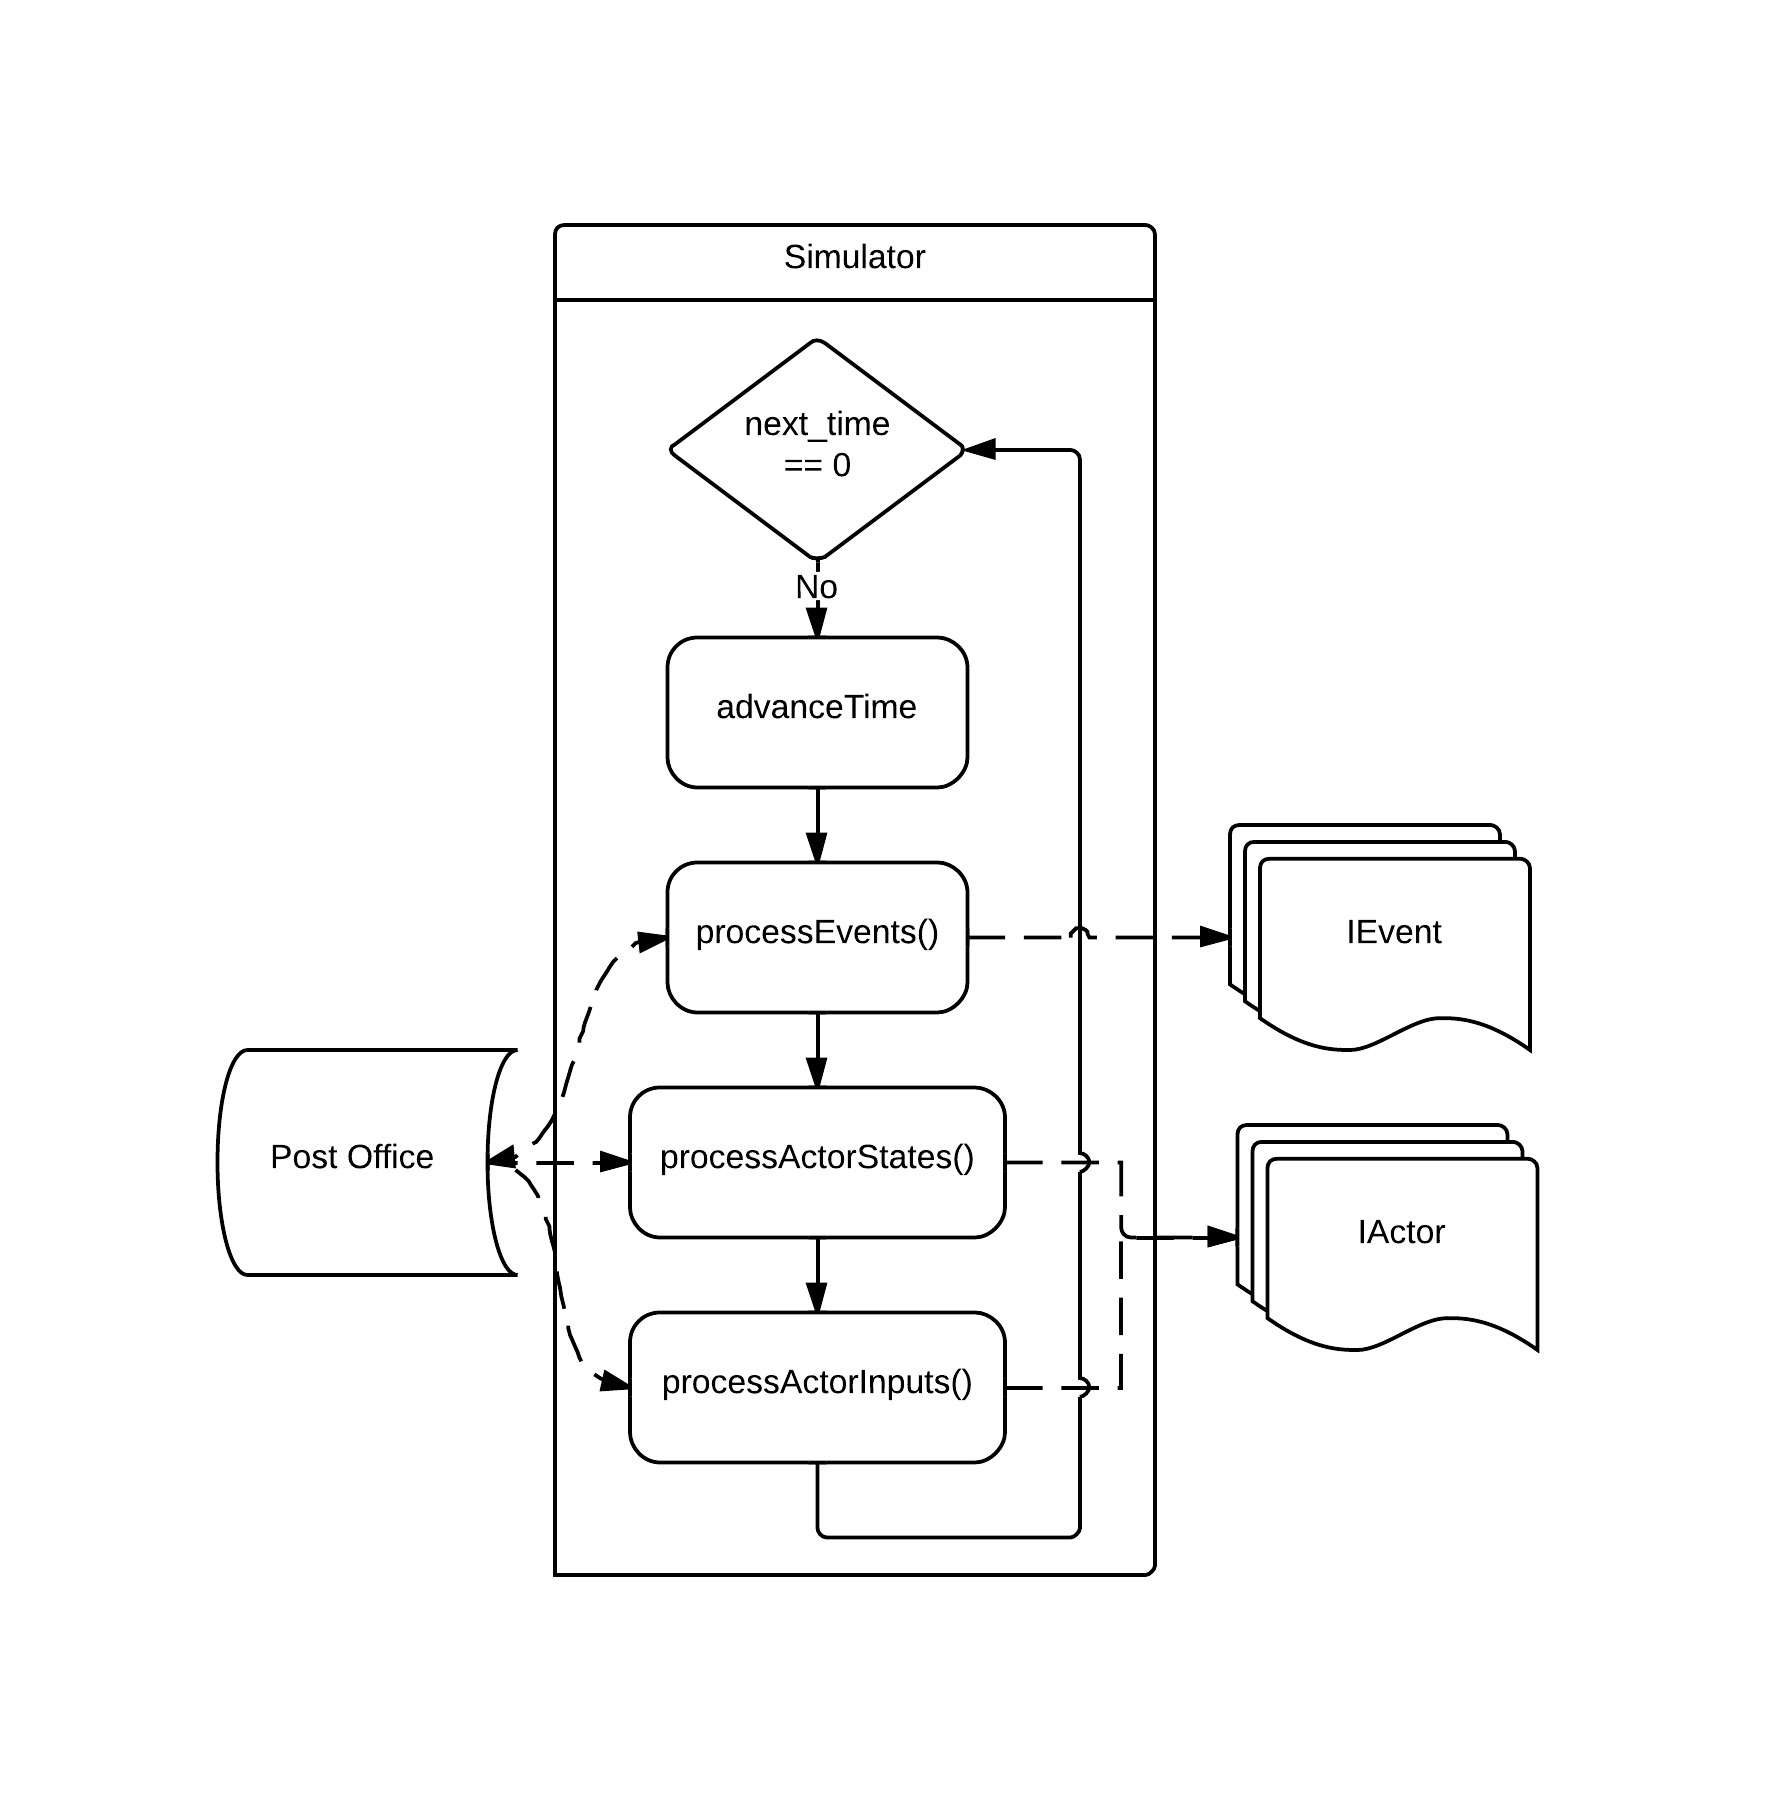
\includegraphics[width=2.5in, trim = 3in 3in 3in 3in, clip]{simulator.jpg}
\caption{Basic simulation timestep}
\label{simulator}
\end{figure}

Figure~\ref{simulator} portrays the execution of a time step. The simulator first processes the next state of any events that undergo a state change in that time. The outputs of those events are stored in the Post Office to be accessed by the Actors when applicable.  Next the simulator calls processInboundData on the PostOffice to move the temporary output to the current output. The Actors then each call processInputs.  Once each Actor has evaluated its inputs and made any changes the simulator checks if there are any future time-steps to evaluate and if not it terminates the simulation.

\subsection{Other Simulation Elements}

To help facilitate the simulation three other interfaces exist.  They are the ITeam, IData, and IState interfaces.  The ITeam interface acts as a wrapper around a team of Actors. The team represents all of the Actors that the simulator will interface with during the simulation and allows the simulator to call a single method on the team to perform actions on all of the Actors. The IData and IState interfaces are used to define common data types for passing information between Actors.  We use enumerations to define outputs and states specific to an Actor. These enumerations implement the correct interface for the type of information they carry.

\begin{verbatim}
public interface ITeam {
    public int getNextStateTime(int);
    public void processNextState();
    public void processInputs();
}

public interface IData {
    public String name();
}

public interface IState {
    public String name();
}
\end{verbatim}

The Simulator class provides a set of helper methods that are accessible to the Actors and Events.  We omit the list of these helper methods in the interest of space.

\begin{verbatim}
int getTime();
void setTime(int time);
int getNextStateTime();
void addOutput(String actor_name,
    IData input);
void addOutputs(String actor,
    ArrayList<IData> inputs);
ArrayList<IData> getInput(String actor);
void linkInput(String parent,
    String child);
void linkObservations(String parent,
    String child);
ArrayList<IData> getObservations(String);
void addObservation(IData data,
    String actor);
void addObservations(ArrayList<IData> data,
    String actor);
void addEvent(IEvent event);
int duration(Range range) ;
\end{verbatim}

This modeling framework imposes no other constraints on the model besides the simulation structure defined by these interfaces.  The model implementation has the full power of the Java language for all internal decision making.  We believe that this will ensure that the framework will be capable of simulating any and all aspects of the UAS model.  This contrasts with semantically constrained modeling languages such as Brahms that, due to the semantics, may not fully map to the model.

\end{comment}


\section{WiSAR UAS Model}
This section describes the models produced for the UAS-enabled WiSAR process.  We first discuss Actors and Events, followed by a brief discussion of Java asserts and a case study drawn from WiSAR.

This conceptual model uses Mealy state machines.  This allows us to abstract the different WiSAR roles into individual state machines that we call Actors.  Actor states do not correspond to a single aspect of the WiSAR domain, thus providing the freedom to flexibly model as many aspects of the domain as necessary and at various levels of resolution. Actors transition between states are triggered by inputs generated by Events and by other Actors.  Events are also modeled as Mealy machines whose transitions are triggered by a combination of simulator and Actor inputs. A benefit of this state machine-based conceptual model is the ability to convert the model into code. The coded model can be verified using model checking tools such as Java Pathfinder (JPF) to gain further insight into the model.  In the interest of space we will not describe the Java simulation framework developed for JPF model checking.

\subsection{Actors}
Choosing the core Actors is critical since modeling UAS-enabled WiSAR requires a level of abstraction that gives useful results without adding unnecessary complexity. After exploring several levels of abstraction, we selected a model that treats as an Actor any core decision-making element of the team, yielding the following Actors: parent search (PS), mission manager (MM), UAV operator (VeOp), video operator (VidOp), UAV operator GUI (VeGUI), video operator GUI (VidGUI), and the UAV.  We deliberately chose to not model ground searchers, leaving this to future work.

The models of the human roles use specific states for communication.  We describe these states once and then refer to them as a single communication state.  Typically before a human communicates he or she receives some signal that the communication is being received.  We model this as a POKE state.  When communicating, an Actor model of a human enters the POKE state where it waits until it receives an acknowledgement. If the acknowledgement is not received then the communication does not occur.  After the acknowledgement the human moves into a transmit (TX) state whose duration is based on the data being transferred.  At the end of this transfer the human enters an end (END) state and outputs the transferred data to the receiver. 

If the Actor model of the human receives a poke, then it responds with a busy or an acknowledge. If the human acknowledges the poke, then it enters the receive (RX) state. The human will not leave this state until the end communication input is received or until it decides to leave on its own. If one of these communications is interrupted before completion, then we consider that the data was not transferred. To better facilitate communication interruptions we only transfer a single piece of information per communication.

The next sections are dedicated to describing the Actor state machines with a generalized description of their relative transition matrixes.  We omit several of the previously mentioned Actors in the interest of space.

\begin{comment}
\begin{figure}
\center
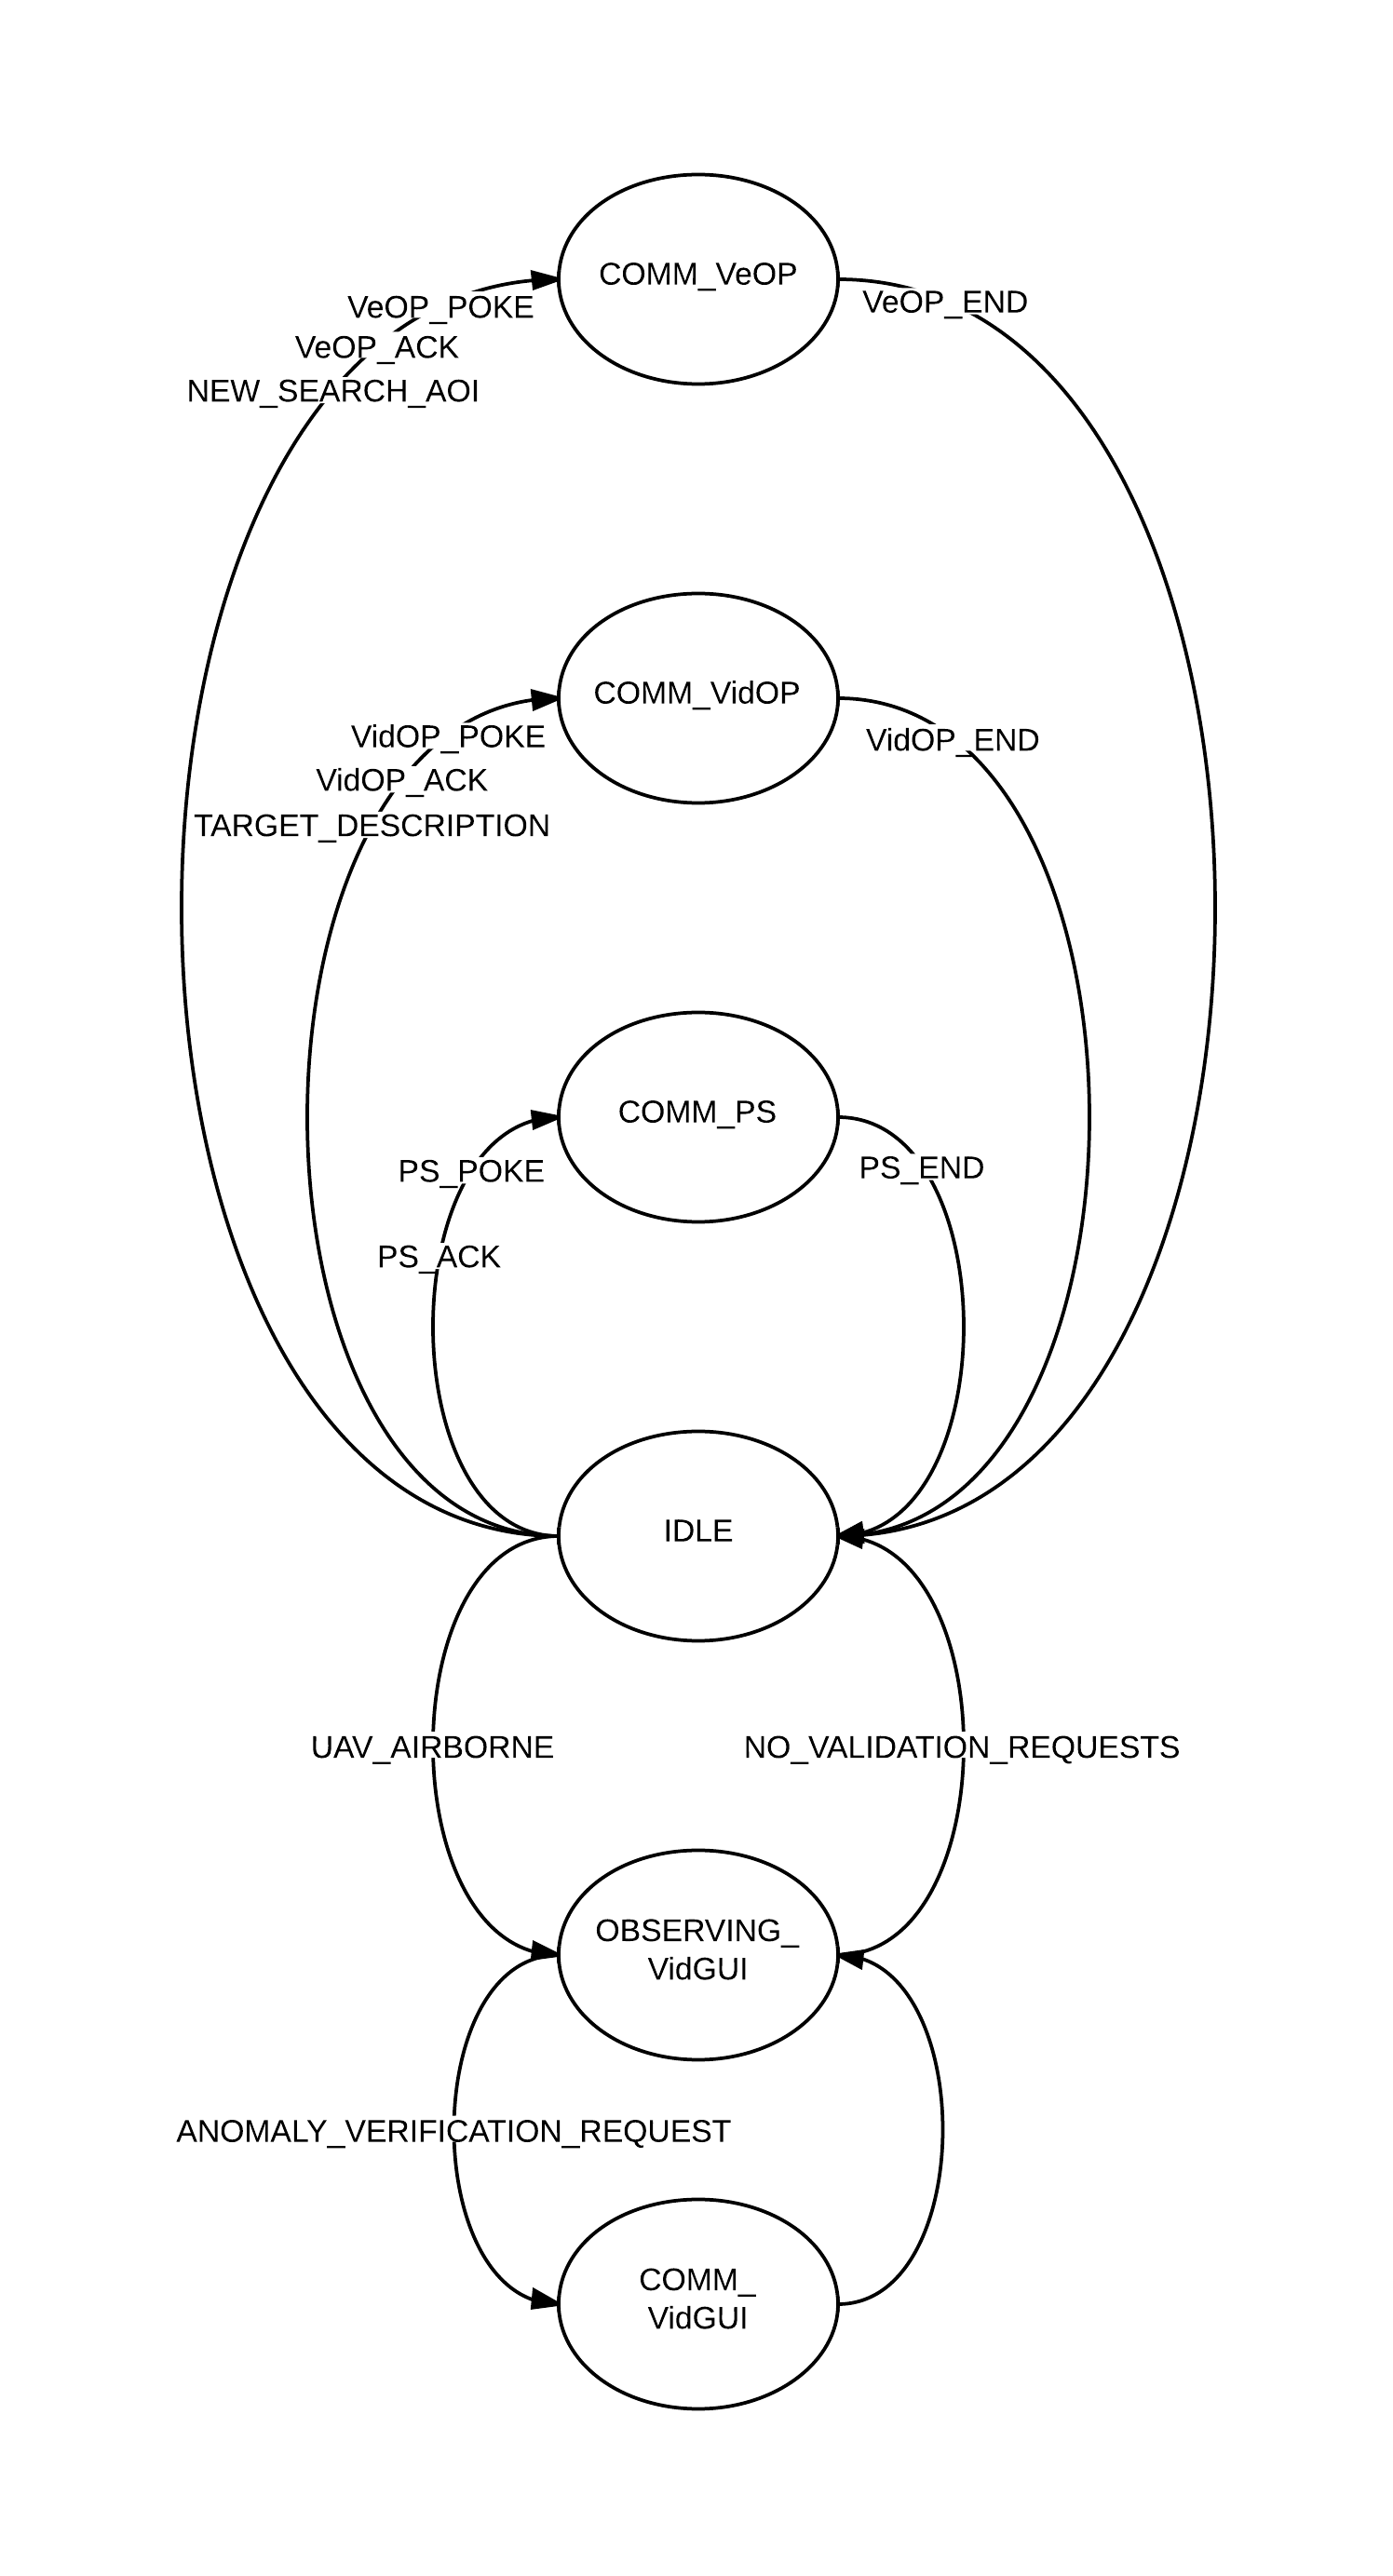
\includegraphics[width=3in]{mm_dirg.png}
\caption{Mission Manager DiRG. Excludes transition output.}
\label{fig:mmdirg}
\end{figure}
\end{comment}

\begin{figure}
\centering
\setlength{\abovecaptionskip}{1mm}
\setlength{\belowcaptionskip}{1mm}
\setlength{\textfloatsep}{1mm}
\setlength{\floatsep}{1mm}
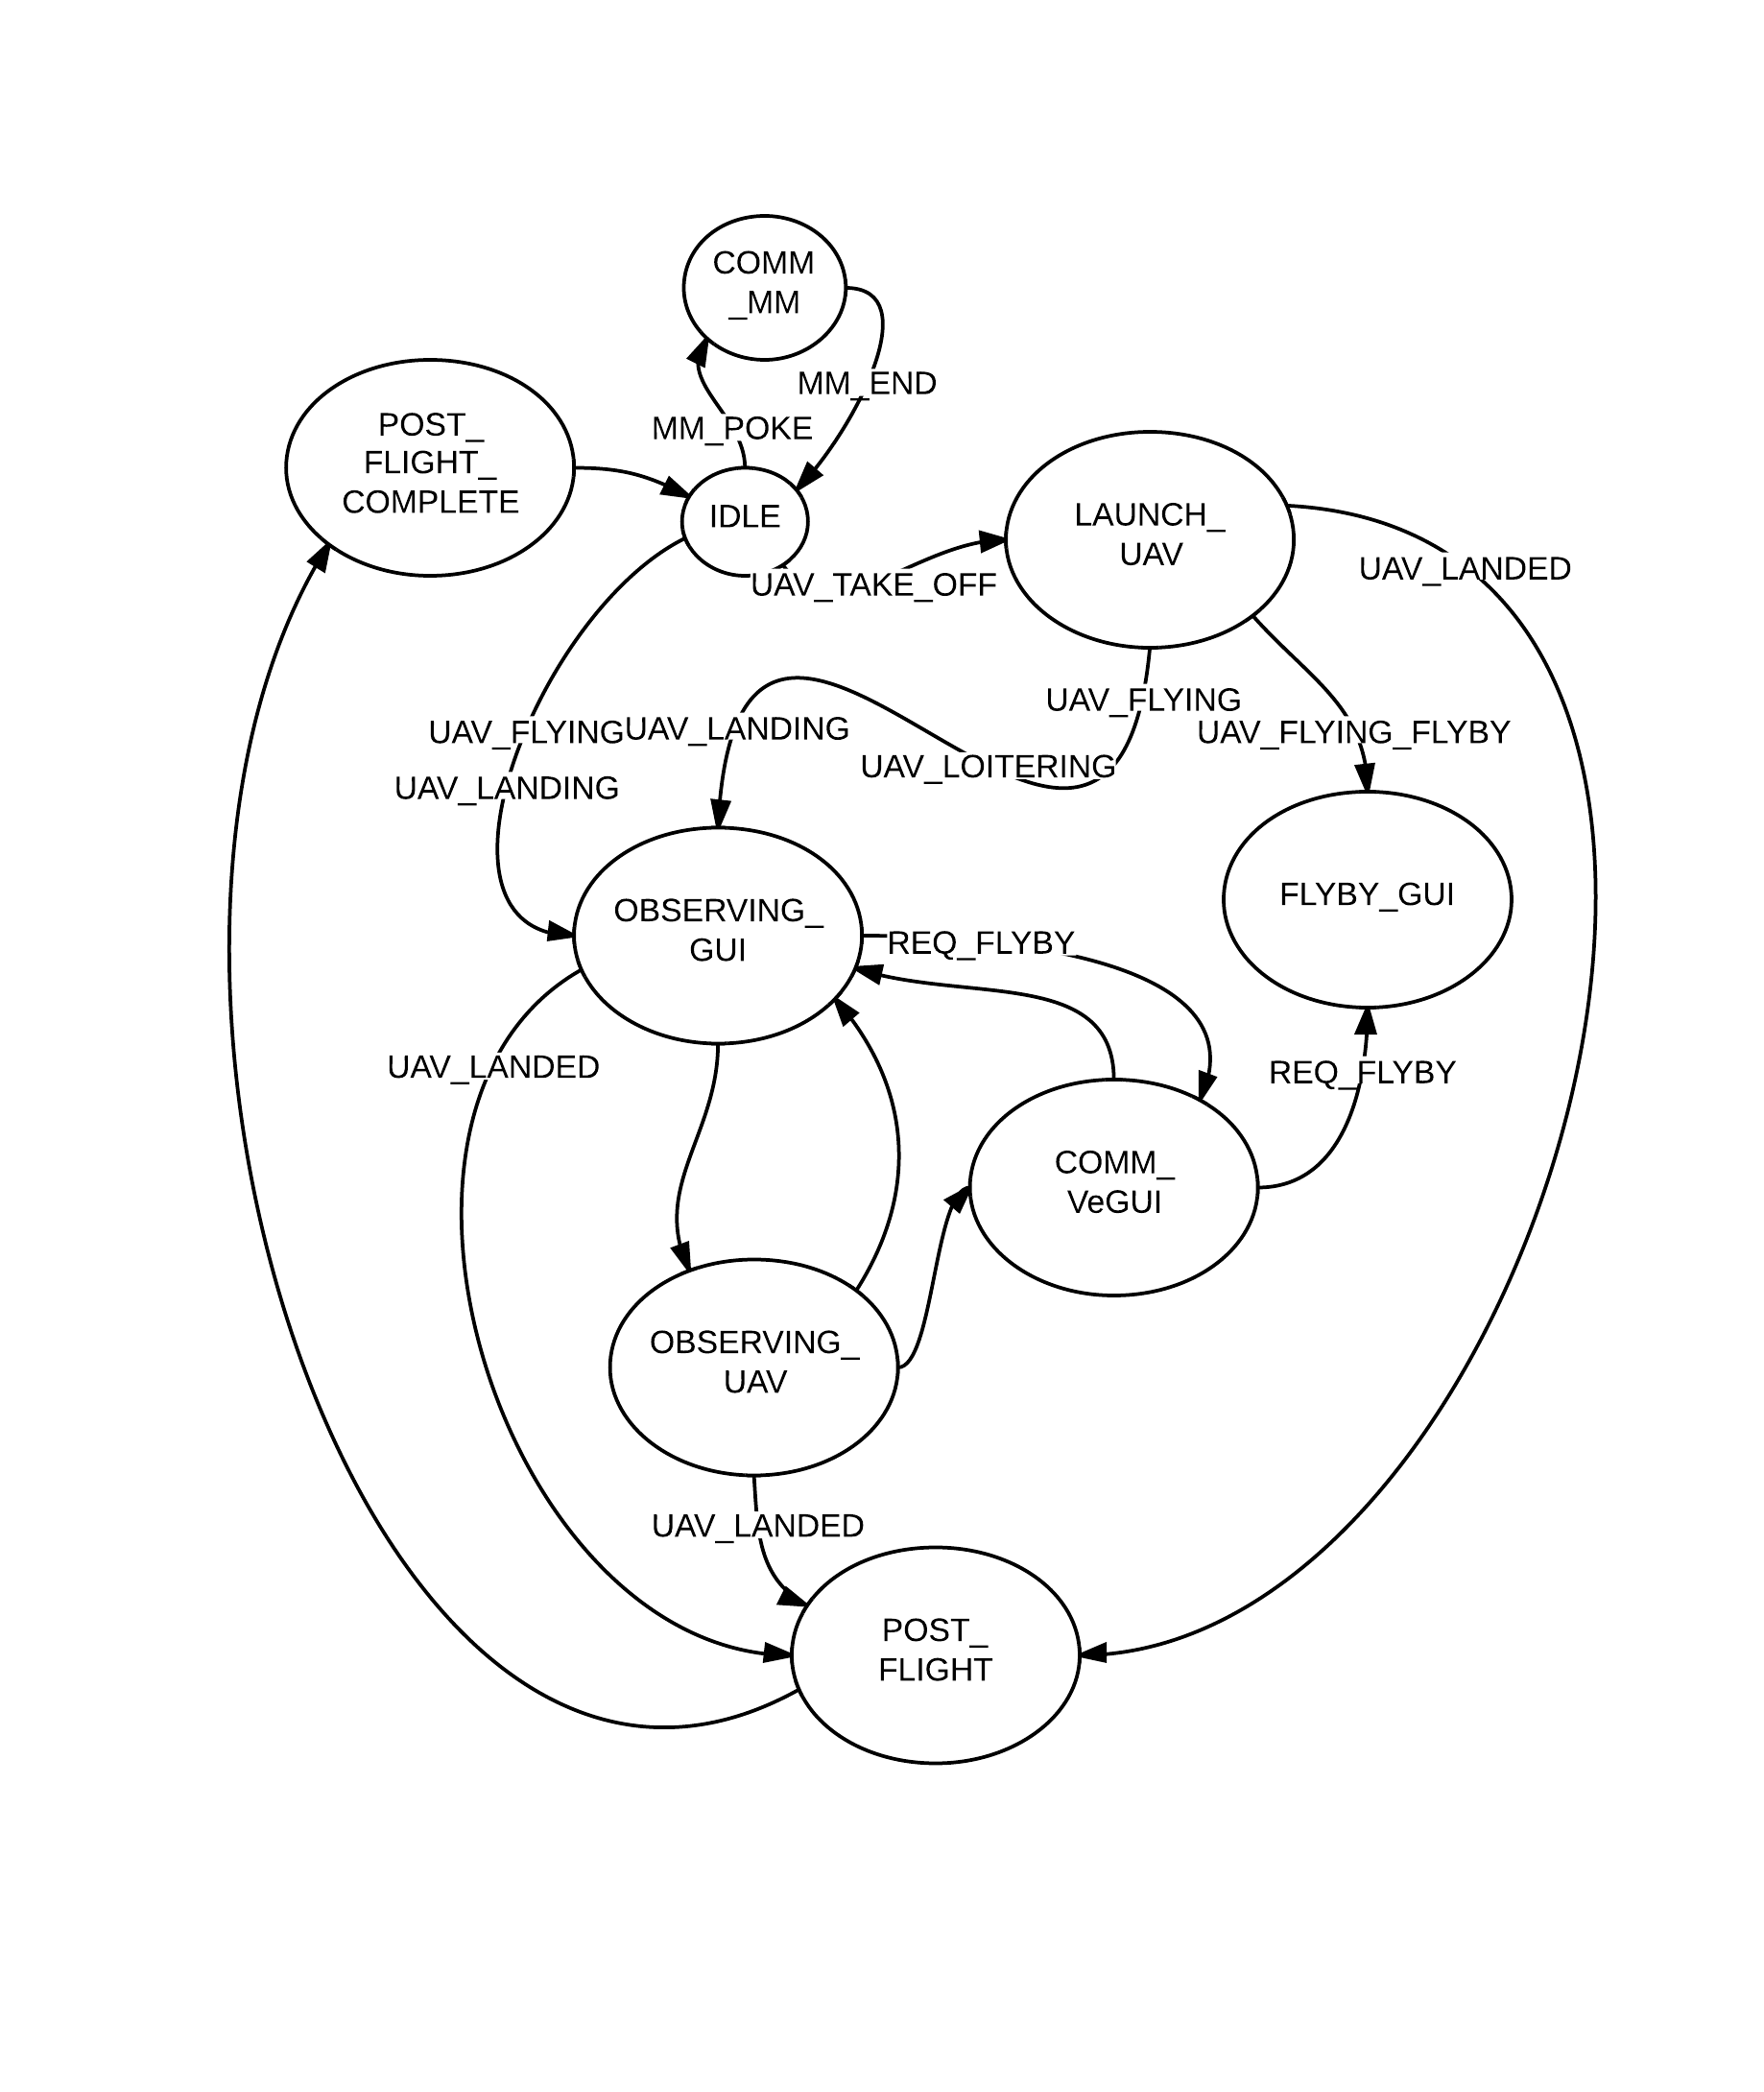
\includegraphics[width=3in, clip, trim=2.5in 4in 2.5in 3in, scale=2]{veop_dirg.png}
\caption{UAV Operator DiRG. Excludes transition output.}
\label{fig:veopdirg}
\end{figure}

\begin{figure}
\center
\setlength{\abovecaptionskip}{1mm}
\setlength{\belowcaptionskip}{1mm}
\setlength{\textfloatsep}{1mm}
\setlength{\floatsep}{1mm}
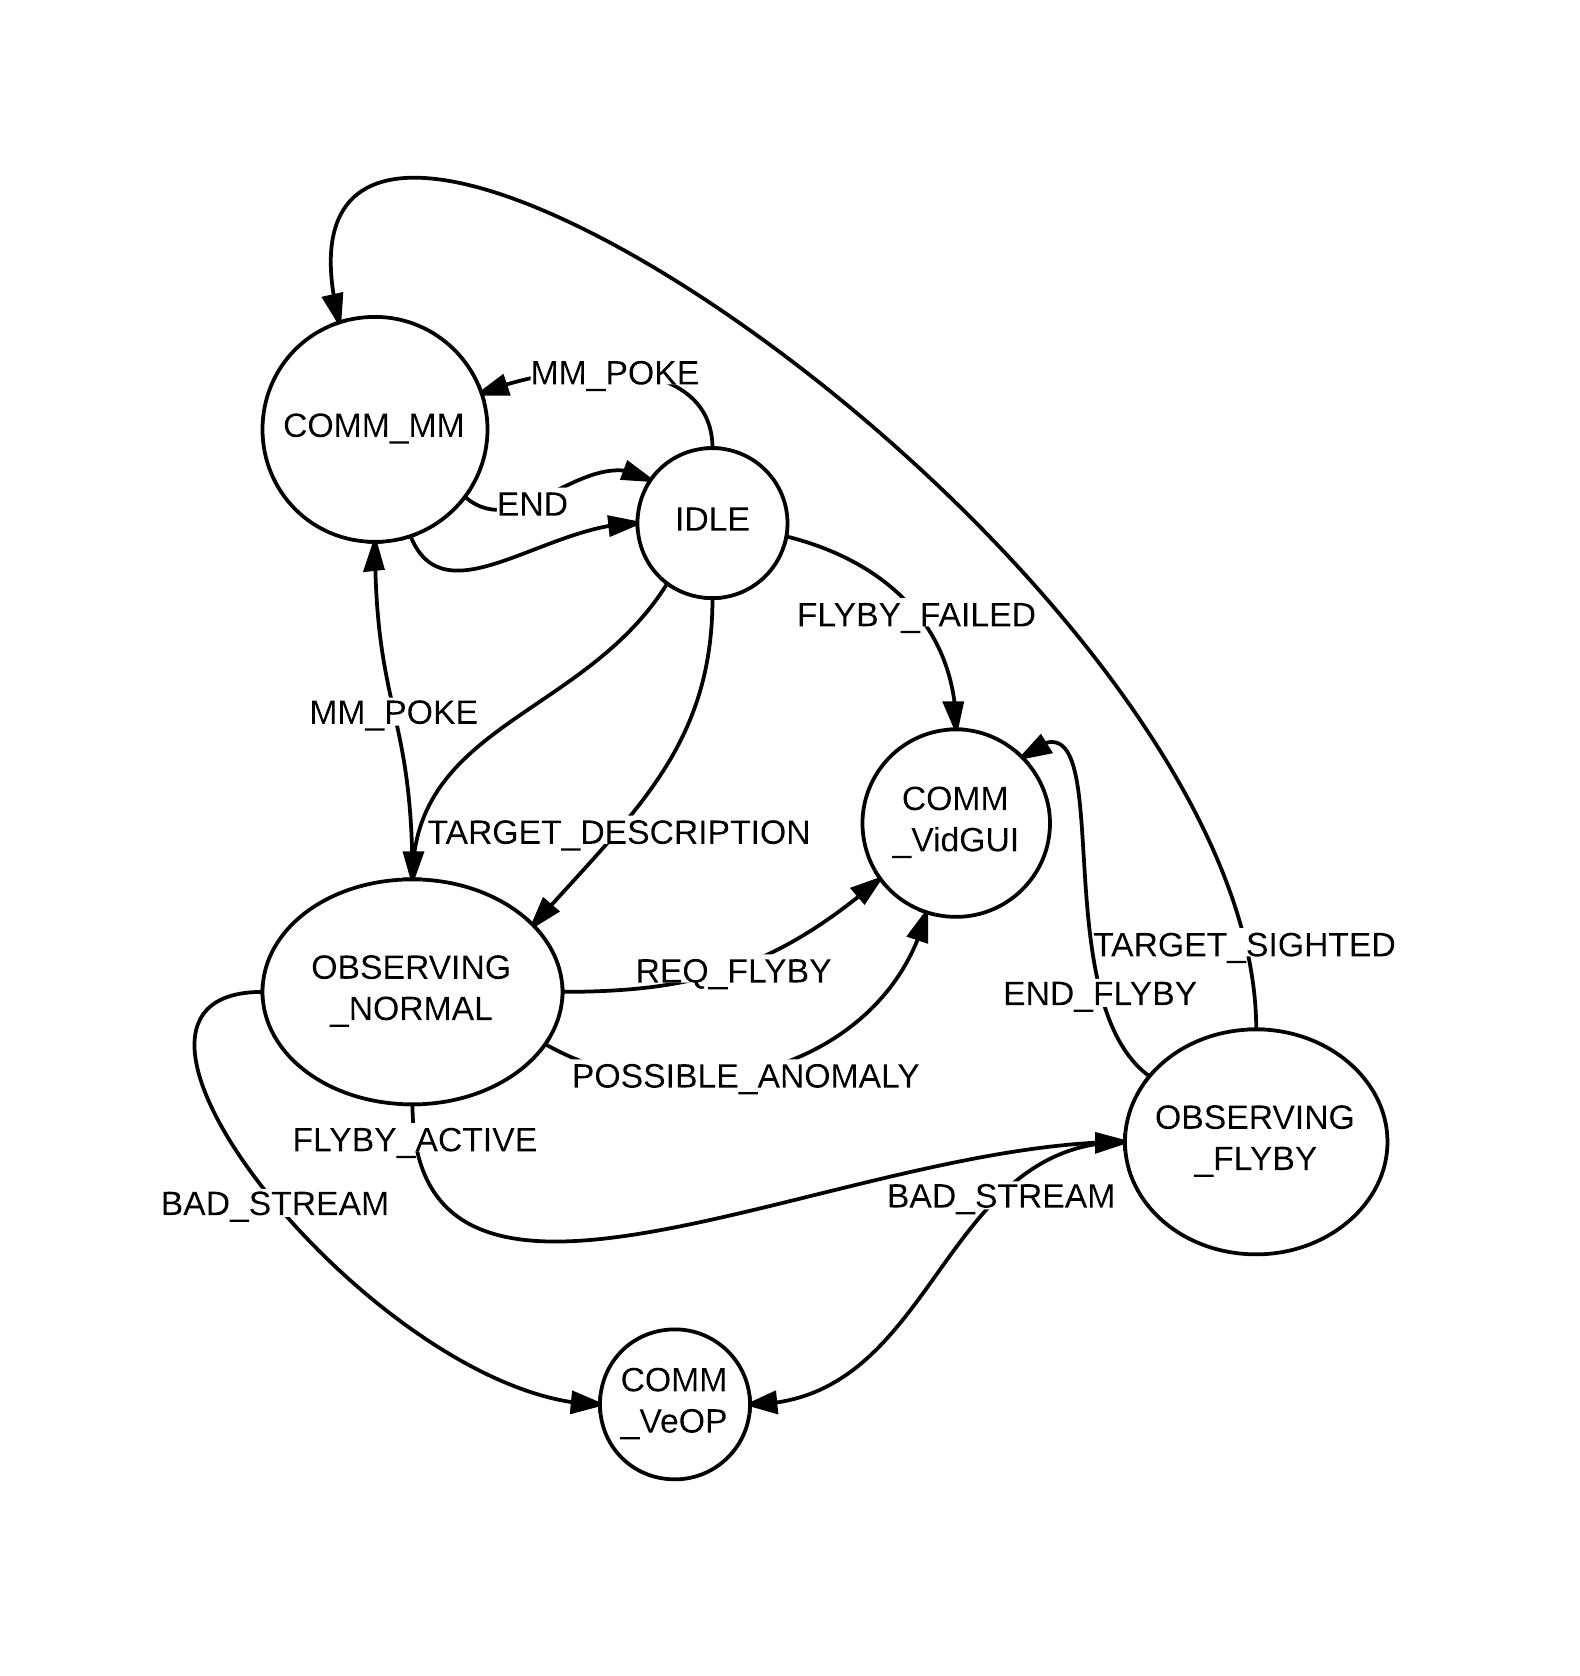
\includegraphics[height=3in, clip, trim=2in 2in 2in 2in]{vidop_dirg.png}
\caption{Video Operator DiRG. Excludes transition output.}
\label{fig:vidopdirg}
\end{figure}


% \subsubsection{Parent Search (PS)}
% This Actor loosely represents the incident commander but is heavily abstracted in our model.  The PS has two main states {\it IDLE} and communicating with the MM.  It contains no logic; it simply passes output from events to the MM and accepts input from the MM.  The events that it listens for are NewSearchAOIEvent, TargetDescriptionEvent, and TerminateSearchEvent described below.

% \subsubsection{Mission Manager (MM)}
% The MM Actor has the following states: {\it IDLE}, {\it OBSERVING\_VidGUI}, and three communication states: {\it PS}, {\it VeOp}, and {\it VidOp}.  Initially the MM is idle. After receiving a new search command and target description the MM distributes the received information. During the search the MM will periodically check the VidGUI to see if there are anomaly verification requests.  For each of these requests the MM will decide if it deserves a flyby or if it is a false positive.  While watching for anomaly verification requests the MM is also listening for input from the PS, VeOp, or VidOp.

\subsubsection{UAV Operator (VeOp)}
As illustrated in Figure~\ref{fig:veopdirg}, the VeOp Actor has the following states: {\it IDLE}, {\it OBSERVING\_VeGUI}, {\it FLYBY\_VeGUI}, {\it OBSERVING\_UAV}, {\it LAUNCH\_UAV}, {\it POST\_FLIGHT}, and three communication states: {\it MM}, {\it VeGUI}, and {\it VidOp}.  Initially the VeOp is idle.  After receiving a new search command from the MM the VeOp constructs a flight plan using the VeGUI.  When this is complete the VeOp will then launch the UAV.  While in the launch state the VeOp is observing the UAV, when the UAV completes its take off the VeOp moves to observing the VeGUI.  While the UAV is airborne the VeOp will continually move between observing the UAV and observing the VeGUI.  The VeOp will respond to any problems that are noticed while observing the VeGUI or UAV.

During the flight the VeOp listens for input from the PS and VidOp.  If there are flyby requests on the VeGUI, then the VeOp may choose to enter a flyby mode.  This implies a high cognitive load on the VeOp while positioning the UAV over the specified anomaly.  The VeOp will remain in flyby mode until the VidOp specifies, through the GUI, that the flyby is finished.  During an operation the UAV will often land and take off multiple times.  The post flight state represents the work necessary to get the UAV ready for flight, such as changing the battery.

\subsubsection{Video Operator (VidOp)}
As illustrated in Figue~\ref{fig:vidopdirg}, the VidOp Actor has the following states: {\it IDLE}, {\it OBSERVING\_VidGUI\_NORMAL},
{\it OBSERVING\_VidGUI\_FLYBY}, and three communication states: {\it MM}, {\it VeOp}, and {\it VidGUI}.  Initially the VidOp is idle.  After receiving a target description and the search information the VidOp moves to normal GUI observation.  While observing the VidGUI the VidOp watches for anomalies, each time an anomaly is visible the VidOp decides if the anomaly is seen.  If it is seen the VidOp decides if it is an unlikely, possible, or likely sighting.  This is done with probabilities related to the type of anomaly, true positive or false positive. If the anomaly is classified as possible then the VidOp makes a validate sighting request for the MM.  If the anomaly is a likely sighting then the VidOp requests a flyby from the VeOp. 

When the VeOp begins a flyby request the VidGUI signals the VidOp to enter the flyby state.  In this state the VidOp watches for the anomaly.  Due to the nature of the flyby the VidOp can now make an informed decision about the nature of the anomaly, gaining a much higher probability of being correct.  After deciding if it is the target the VidOp signals through the VidGUI that the flyby is finished.  If the sighting is confirmed the VidOp reports to the MM, otherwise the VidOp returns to normal GUI observation.

\subsubsection{Operator GUI (VeGUI)}
The VeGUI Actor has two states: {\it NORMAL} and {\it ALARM}. The VeGUI communicates directly with the UAV and VidGUI Actors. The default function of the VeGUI is to observe the UAV. The VeGUI keeps internal variables of all the UAV and VidGUI data that it tracks, all of this data is available through observation of the VeGUI.  If it detects an error with the UAV outputs such as low battery, no flight plan, low height above ground, or lost signal the VeGUI will enter the alarm state.  This state indicates that there are visible warnings on the screen to alert the VeOp of the problem.  The VeGUI listens for VeOp input or changes in the UAV output to signal that the problem has been dealt with before moving into the normal state.

% \subsubsection{Video Operator GUI (VidGUI)}
% The VidGUI Actor has two states: {\it NORMAL} and {\it FLYBY}.  The VidGUI has the same communication model as the VeGUI.  The default function of the VidGUI is to present anomalies to the VidOp.  The VidGUI presents anomalies by listening for input from TruePositiveAnomalyEvent and FalsePositiveAnomalyEvent.  The VidGUI tracks the visible anomalies, flyby requests, and anomaly verification requests.  The VidGUI moves to the flyby state after the VeOp initiates a flyby.  In this state the VidOp can observe that the UAV is attempting to relocate and obtain better video quality of a previously seen anomaly.  The VidGUI will remain in this state until it receives the finished command from the VidOp.  

\subsubsection{UAV}
The UAV Actor has the following states: {\it READY}, {\it TAKE\_OFF}, {\it FLYING}, {\it LOITERING},
{\it LANDING}, {\it LANDED} and {\it CRASHED}.  Initially the UAV is in the ready state.  Upon command the UAV moves to take off for a specific duration and then to flying or loitering.  The flying state is when the UAV is following a flight plan.  The loitering state is when the UAV is circling a specific location.  The UAV will automatically enter the loitering state after completing its flight plans.  While airborne the UAV, upon command, moves to the landing state for a specific duration before moving into the landed state.  Once landed the UAV must be moved into the ready state before it can take off again.

The Actors in this model, thus far, represent a fairly high level of abstraction.  Fortunately, the DiRG conceptual framework allows incremental extension of the models by adding lower levels of abstraction.  This is accomplished by introducing {\em sub-Actors} into the model.  We illustrate how the Actor/sub-Actor hierarchy can be used by describing two UAV sub-Actors.  In these examples the sub-Actors receive all the same input as the parent Actor and all sub-Actor output is sent from the parent Actor.

The first UAV sub-Actor is the UAVBattery. It contains the following states: {\it INACTIVE}, {\it ACTIVE}, {\it LOW}, and {\it DEAD}.  Initially the battery is inactive.  The battery is assigned a duration and a low battery threshold.  When the UAV receives the take off command the battery enters the active state.   The batteries next state is set to low at time $current\_time +  battery\_duration - low\_battery\_threshold$.  When the battery enters the low state its next state is set to dead at time $current\_time + low\_battery\_threshold$.

A second sub-Actor is the UAVFlightPlan. This represents the flight plan flown by the UAV. The flight plan requires a specific amount of time to complete.  The UAVFlightPlan has the following states: {\it NONE}, {\it ACTIVE}, {\it PAUSED}, and {\it COMPLETE}.  Initially the flight plan is set to none. After the operator creates a flight plan using the VeGUI then the flight plan moves to active.  During a flight the UAV may loiter, land, or flyby; this causes the flight plan to move to paused. When the UAV begins following the flight plan again it returns to active. After the UAV has flown the flight plan for the specified duration the flight plan enters the complete state.

The results discussed below include four other UAV sub-Actors: UAVHeightAboveGround, UAVSignal, UAVVidFeed, and FlybyAnomaly.  Details are omitted in the interest of space.

%The next sub-Actor is the UAVHeightAboveGround which has the following states: {\it INACTIVE}, {\it GOOD}, {\it LOW}, and {\it CRASHED}.  Its initial state is inactive..  This Actor represents the UAVs height above the ground (HAG).  Its main purpose is to listen for low height above ground events and to crash the UAV if a response is not received in time.  Once the UAV is airborne the HAG will remain good unless input is received from the LowHAGEvent.  The event moves the UAVHeightAboveGround into the low state.  If the UAV receives a modified flight plan then the state is changed back to good, otherwise the UAV will crash when it receives the second output from the LowHAGEvent..

%The next sub-Actor is the UAVSignal which has the folowing states: {\it OK} and {\it LOST}.  Initially it is set to OK.  This represents the UAVs communication with the VeGUI.  Its main purpose is to handle input from LostSignalEvent.  When this event occurs the signal enters the lost state until receiving input to return to the ok state.

%The next sub-Actor is the UAVVideoFeed which has the following states: {\it IDLE}, {\it OK} and {\it BAD}. This represents the quality of the UAV video feed.  Its purpose is to handle BadVideoFeedEvents. Its initial state is idle.  When the UAV takes off the video feed moves to OK.  When a BadVideoFeedEvent input is received the video feed moves to bad.  This is only returned to OK after the UAV has landed and taken off again.  Whenever the UAV is on the ground the state moves to idle.

%The last sub-Actor is the FlybyAnomaly which has the following states: {\it IDLE}, {\it ANOMALY\_NOT\_SEEN}, {\it ANOMALY\_SEEN}, {\it PAUSED}, and {\it FLYBY\_COMPLETE}.  This represents when the UAV is performing a flyby of a previously seen anomaly. Initially it is set to idle, indicating a flyby is not being executed. When a flyby is begun the FlybyAnomaly Actor moves into the anomaly not seen state for a specified duration before moving into the anomaly seen state, where it remains until the end flyby command is received.  During the anomaly seen state we assume that the anomaly is visible from the UAV and that it will remain visible until the flyby is complete.  When the end flyby command is received the FlybyAnomaly briefly enters the flyby complete state before returning back to idle.  If the UAV needs to land or loiter for any reason during the flyby it will enter a paused state.

\subsection{Events}
We used the Event Abstraction for several different elements of the UAS-enabled WiSAR problem. Adding this abstraction allows humans analyzing the system to give a set of inputs to the model and observe the consequences of the inputs.

\begin{comment}
Since all events behave similarly, despite the two classes of abstractions, we created a single state space that all Events use. Events have the following states:  {\it INACTIVE}, {\it ACTIVE}, and {\it FINISHED} (see figure~\ref{fig:eventdirg}). Initially all Events are inactive.  While inactive an Event will check to see if it is possible.  If the Event is possible then a timer is set to move the Event to active at some arbitrary future time; this allows Events to be triggered non-deterministically.  If the Event becomes impossible before becoming active the timer is removed.  Otherwise when it enters the active state its designated outputs are triggered and a timer is set for when it leaves the active state and enters the finished state.  At that point it outputs a signal indicating the event has terminated and returns to the inactive state. If there are multiple events, then it restarts the cycle until it has triggered a sufficient number of times.
 
\begin{figure}
\center
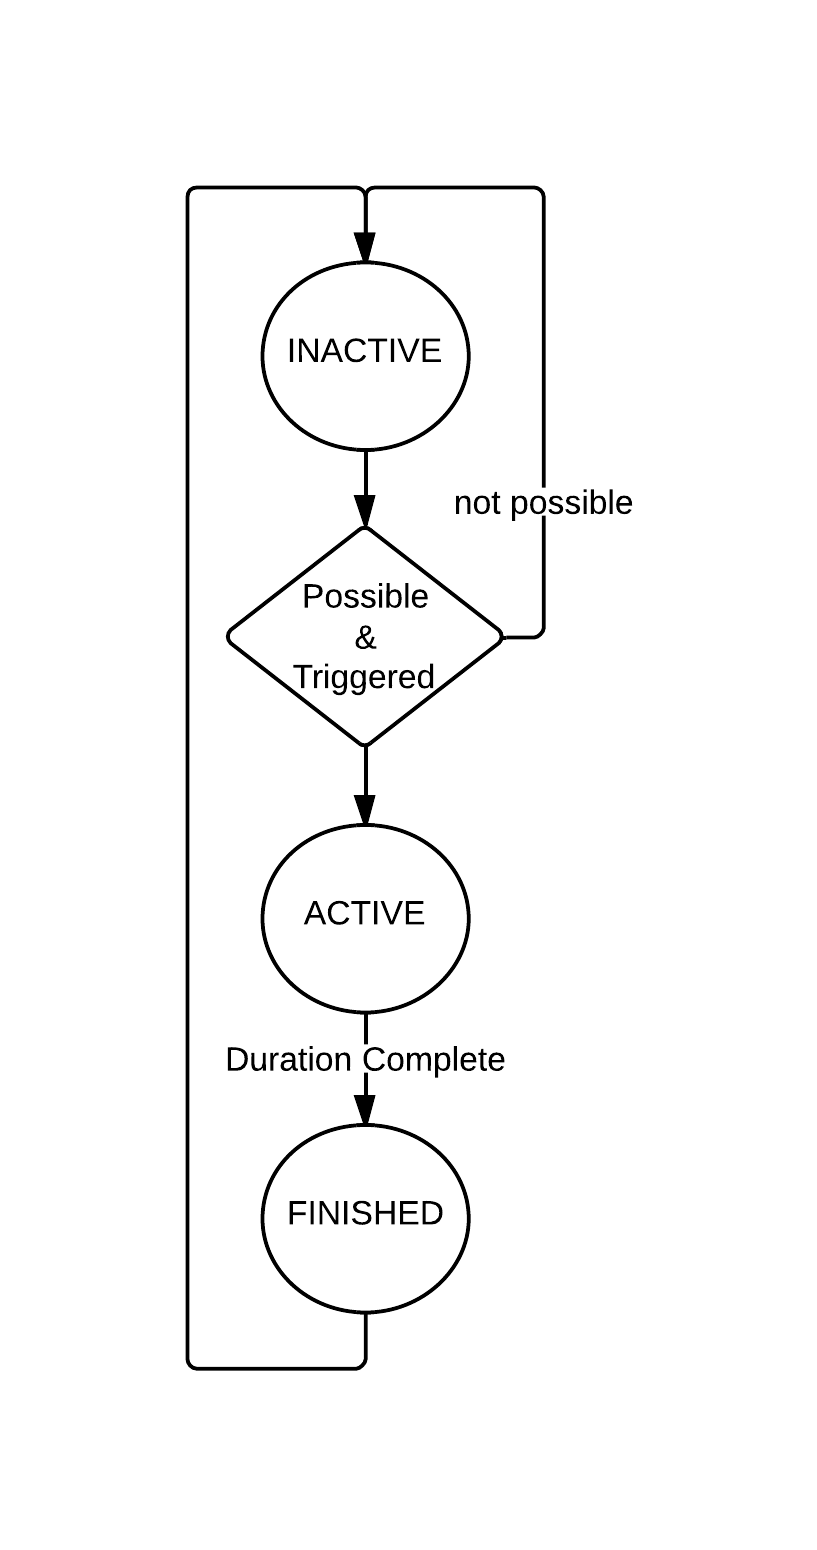
\includegraphics[width=2in]{event_dirg.png}
\caption{Event DiRG. Excludes transition output.}
\label{fig:eventdirg}
\end{figure} 
\end{comment}
The following Events were encountered in various UAS-enabled WiSAR field trials and represent a sample of interesting possible operating conditions for the Actors.  In the interest of space we list these events while omitting their descriptions.
NewSearchAOIEvent, TargetDescriptionEvent, TerminateSearchEvent, LowHAGEvent, LostSignalEvent, TruePositiveAnomalyEvent, FalsePositiveAnomalyEvent, and BadVideoFeedEvent.\footnote{HAG = Height Above Ground, AOI = Area of Interest}
\begin{comment}
\subsubsection{NewSearchAOIEvent}
This event outputs a new search area of interest (AOI) to the PS.  The VeOp cannot perform its duties until this output is received.
\subsubsection{TargetDescriptionEvent}
This event outputs a target description to the PS.  The VidOp cannot perform their duties until this output is received.
\subsubsection{TerminateSearchEvent}
This event outputs a terminate command to the PS.  The parent search may terminate for a multitude of reasons and at anytime.
\subsubsection{LowHAGEvent}
This event is only available while the UAV is airborne, it outputs height above ground(HAG) is low.  This event sends a second output after a specified period indicating that the UAV crashed.  This output is ignored if the flight plan was modified.
\subsubsection{LostSignalEvent}
This event is only available while the UAV is airborne.  It first sends a lost signal output.  After a specified duration it then sends an ok signal output.
\subsubsection{TruePositiveAnomalyEvent}
Only possible while the UAV is flying its flight plan.  Outputs an initial signal that the anomaly is visible.  Outputs a second signal that the anomaly is no longer visible.
\subsubsection{FalsePositiveAnomalyEvent}
Same process as TruePositiveAnomalyEvent.
\subsubsection{BadVideoFeedEvent}
Only available while the UAVVideoFeed is ok.  Outputs that the video quality is now too poor to be effective.
\end{comment}

\subsection{Asserts}
As a general rule in model-checking, the more complex the model the more that can go wrong. Detecting flaws in the model is extremely valuable because such flaws trigger further evaluation.  We present a case study in the next section that illustrates how the evaluation can identify things that need to change in the WiSAR process to avoid serious errors and perhaps failure to find the missing person.  

Unfortunately, it can be challenging to differentiate between important flaws and coding bugs.  To catch all errors, both flaws and bugs, we use Java Asserts. JPF automatically halts processing when it
encounters a false assertion, allowing us to determine if the error is a bug or
a flaw.

The model uses asserts in two ways. The first is detection of an
undesired state. If an actor enters an undesirable state then an assertion halts
the simulation. An example of this is the {\it UAV\_CRASHED} state. The second deals with inputs. Many operations are sequential.  They require a specific state and input before the next task can be performed. By looking at an Actors received inputs we are able to tell if an Actor is out of sync with the other Actors. An example of this
is the {\it VeOp\_TAKE\_OFF} input for the UAV. If the UAV is already airborne and it
receives this input we know that the operator is out of sync with the UAV.

Asserts are critical to debugging and verifying of the model.  We found that
having too many asserts is preferable to having too few.

\subsection{Case Study: Anomaly Detection}
The scenario illustrated in figure~\ref{state_machine} represents a portion of what should occur when the video operator believes a target has appeared on the video GUI. Each vertical swimlane represents an Actor/ DiRG.  Periodically during a flight the UAV will fly over an anomaly.  An anomaly can be either a false positive or a true positive,  meaning that it is either the desired target or it is not.  If the video operator believes that it is the target then a flyby request is made through the video GUI.  This request is then made visible to the operator through the operator GUI.  When the operator decides to perform the flyby request he signals this through the operator GUI and begins to manually direct the UAV to the location of the anomaly.  While the operator is directing the UAV the video operator closely examines the video stream until the anomaly is visible again.  The video operator then decides if it is a true target sighting or a false positive.  The video operator communicates this to the operator through the video GUI.  If it was a target sighting then the video operator passes the information to the mission manager who then passes it to the parent search. This high level view communicates the basic structure of the communication between the different actors.

\begin{figure}
\center
\setlength{\abovecaptionskip}{1mm}
\setlength{\belowcaptionskip}{1mm}
\setlength{\textfloatsep}{1mm}
\setlength{\floatsep}{1mm}
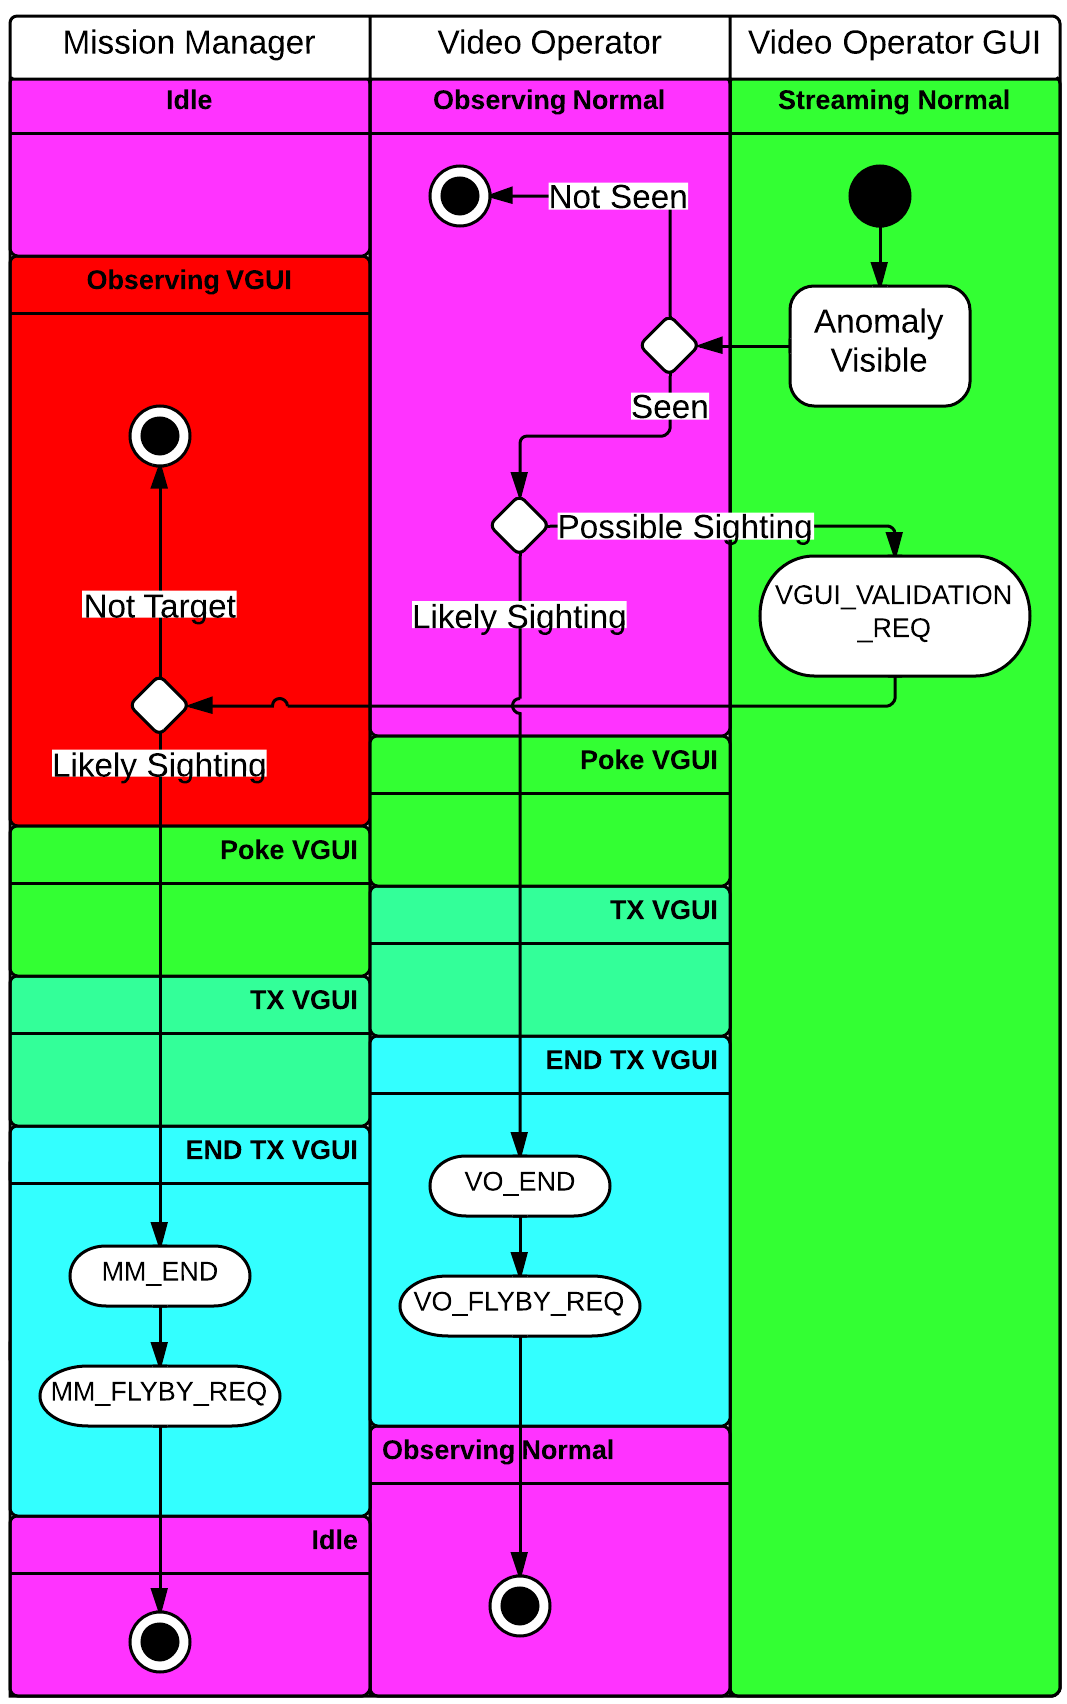
\includegraphics[width=5in]{state_machine.png}
\caption{Anomaly Detection Model: Swim lanes represent actors.  Arrows
represent input/output.  Colored sections represent actor states.}
\label{state_machine}
\end{figure}


\section{Results}
%In this section we present empirical results to demonstrate that WiSAR UAS is
%modeled effectively using the approach we have taken.
%We will demonstrate this using a brief case study extracted from WiSAR UAS.  We
%will then give an analysis of the JPF results we obtained when we verified the
%model.

In this section, we first discuss model-checking results and then present insights from the modeling process.

%\subsection{Model Construction}
%As mentioned in section $V$ we use seven core actors in our model.  The anomaly detection effects each of these actors.  %Because we already had the core actor classes setup before we defined this part of the model it was a simple process of  %adding additional states and transitions to our actors.  For the anomalies themselves we created an anomaly event which sent %output directly to the video GUI.  We wanted the operator to non-deterministically choose if an anomaly was not seen, seen as %a possible target, or seen as a likely target.  We were able to achieve this by generating a random probability within a %designated range.  This means that when run by JPF each of those probabilities will be explored.  A small portion of the model %can be seen in
%figure~\ref{state_machine}.





\subsection{JPF Results}
Model checking constructs an exhaustive proof, by enumerating every reachable state of a system, to establish a property. The JPF model checker uses native Java as the modeling language to describe a system, and implements a custom virtual machine to systematically explore the reachable state space of the compiled Java program. The reachable state space of a sequential model is trivial to enumerate but the reachable state space grows exponentially with the level of non-determinism (i.e., random choice).

The source of non-determinism in the WiSAR model is in timing. The model defines time bounds for different events and tasks in the system. When the model is run, it non-deterministically chooses delays from within those bounds. For example, the time to land the UAV is a uniform random variable bounded between 60 and 1,800 time units. In the WiSAR model, there are 69 different tasks or events with non-deterministic durations. As it is not feasible to enumerate the entire reachable state space of such a large model, this work implements several standard heuristics to limit the non-determinism: minimum(maximum) time only;  minimum and maximum times only; and minimum, maximum, and mean times only. As expected, the first heuristic using only the minimum(maximum) time bound results in a sequential model with no non-determinism.

The total number of meaningful lines of code, code within methods, for the WiSAR model is 3,804. JPF is able to analyze the model using the minimum heuristic in negligible time only enumerating 124 states on a MacBook Air with 4GB of memory and an Intel Core I7 1.6 Ghz processor. The maximum heuristic also has negligible time but fewer behaviors with only 16 states. The difference in states is due to the UAV not needing to land several times to recharge its battery. 

The minimum and maximum bounds heuristic in JPF generates an important and interesting result. JPF finds a combination of task durations that result in an infinite loop using the heuristic. The same infinite loop can be recreated outside of JPF by repeatedly running the model over and over again as random trials until one of the trails goes into an infinite loop. The power of using JPF is that it finds the infinite loop every time without the need for the random trials. The root cause of the infinite loop was a flawed communication protocol that implicitly relied on specific delays in the interaction.  The protocol has since been corrected and JPF verifies the model to now terminate under all combinations of minimum or maximum delays: 3,911 states in 6 seconds of running time. 

The greatest number of states enumerated by JPF comes  from using the minimum, maximum, and mean heuristic. For all 69 points of non-determinism in the WiSAR model, JPF exhaustively considers 3 distinct values for each point, and checks every possible combination. JPF enumerates 51,344 states in around 52 seconds using the heuristic. None of the states violate the current set of assertions in the model and the model terminates under all the duration combinations. The jump in the number of states between the minimum and maximum bounds heuristic and this heuristic illustrates the exponential state explosion inherent in model checking. 

The JPF model checking does not prove the WiSAR model is the desired model or even a correct working model. There is considerable research yet to be completed in writing the system level requirements of WiSAR and then having JPF verify each of those requirements. If JPF finds a violation on any given requirement, there is still considerable work to determine if the requirement is correct (i.e., really what is desired from the system), if the model has a bug, or if the protocols in the model are fundamentally flawed and not able to implement the requirement. These topics are future work for the WiSAR model.

\begin{comment}
 In the context of the WiSAR model, model checking systematically enumerates every reachable state of the model in an effort to violate user defined assertions. 

The model contains 69 task duration ranges. A duration range defines a relative minimum and maximum time needed to complete a task.  Each time the model requests a duration the simulator non-deterministically returns a value from that range based on the simulation settings.  See Table~\ref{tab:jpf}.  JPF made it possible to explore the different paths created by the non-deterministic task durations.  

The entire Java code base consists of  $22,166$ lines of code which includes everything but spaces.  If looking at just lines of code within methods (LOCm), which represents the interface implementations, the number of key lines of code drops to $3804$.  See Table~\ref{tab:code}.   We ran our model checking on a MacBook Air with 4GB of memory and a 1.6Ghz Intel Core I7 processor.  With deterministic task durations we found a significant difference in the new states between the {\it MIN} and {\it MAX} durations.  When we increased the non-determinism, the number of new states exploded (see {\it MIN\_OR\_MAX} vs {\it MIN\_MEAN\_OR\_MAX}). See Table~\ref{tab:jpf}.  

These results were generated using a simplified version of our model, fewer Events and assertions, which runs to completion.  That is, a search area is received, the team searches the area finding nothing, and the PS is informed.  While the lack of assertions and other output makes it difficult to interpret these results they begin to show us how we can gain insight into WiSAR.  The difference between the number of new states between {\it MIN} and {\it MAX} durations tells us it takes more tasks to complete the same thing when task duration is lowered.  By using {\it MIN\_OR\_MAX} or {\it MIN\_MEAN\_OR\_MAX} JPF can automatically tell us which of those durations causes the greatest increase in new states.  In this particular scenario the minimum UAV battery duration forced the UAV to land several times to complete the same search.
\end{comment}

\begin{comment}
\begin{table*}
\begin{center}
\caption{metrics obtained using  the EclipseMetrics plugin}
\label{tab:code}
\begin{tabular}{ l || c c c c c c c c}
 & LINE & LOCm & CC & NOS & NLS & NOL & FE  NOP \\
\hline\\
Simulator & 5327 & 715 & 160 & 413 & 10 & 129 & 16 & 56 \\
Model & 16839 & 3089 & 740 & 2684 & 1 & 311 & 249 & 37 \\
Total & 22166 & 3804 & 900 & 3097 & 11 & 440 & 265 & 93 \\
\end{tabular}
\end{center}
\end{table*}
\end{comment}

\begin{comment}
There were a few cases when JPF would enter an infinite loop.  In two of these cases we found that we had an error in our model.  The first error occurred because an Actor was not receiving the input necessary to transition properly.  The second error occurred because we had an implicit transition instead of an explicit transition.  From this we learned the importance of expressing transitions explicitly and in validating the connectivity of the model which we plan to implement as future upgrades to our simulator.
\end{comment}

\subsection{Lessons from Modeling}
One of the goals of using model-checking with UAS-enabled WiSAR is to discover problems and opportunities with the structure of the organization.  This section presents several important lessons for UAS-enabled WiSAR that were obtained through the modeling exercise. 

First, while modeling the VidOp it became apparent that there was a problem with the organization.  This problem occurs because, while the VidOp is marking an anomaly, the video feed continues to run. This means that it is possible that the VidOp may miss detecting the target.  If the VidOp pauses the video, the feed falls behind the live video feed which makes flyby requests more expensive because the UAV will have to backtrack to the anomaly sighting.   We analyzed why this problem was not discovered in the WiSAR field trials.  The answer is that the field trials included multiple video feeds with multiple observers, a condition that is not likely to occur in a resource-limited search.  A lesson from this observation for WiSAR is that technology needs to be developed that allows the WiSAR team to manage this problem.  A more general lesson is that the modeling and model-checking process uncovered a potential problem before it appeared in practice.

A second lesson was learned when performing model-checking of a flyby.  Our model showed two problems, resuming a flight plan after a flyby and needing to keep a list of flyby requests.  We solved this in the model by adding visible queues to the VeGUI and VidGUI and allowing the VeGUI to store multiple flight plans.  As before, we analyzed why these problems were not discovered in the WiSAR field trials.  The answer is that these problems did occur but were not documented. The lesson for WiSAR is that the VeGUI and VidGUI need new features to support real searches.   A broader lesson is that the modeling exercise can be used to not only detect problems but specify the requirements for fixing them.

\begin{comment}
We add to these two specific lessons two meta-observations about creating an effectual process for modeling the system.  First, the exercise reminds us of the fact that verification is only as good as the questions asked.  Our initial success when the model ran to completion was tempered when we realized that it only implied that the code ran.  To obtain insight into specific aspects of the WiSAR UAS questions must first be described as assertions and outputs inside the model.

The second meta-observation is that the modeling approach needs to be able to be scalable to different levels of abstraction and different possible implementations of the system.  Through the modeling process, we can replace, change, and ignore processes or levels of detail.  This allows us to use scalable DiRGS to explore the ``what if's '' of the system instead of constraining ourselves to what currently happens with a system.
\end{comment}

\begin{comment}
\begin{table*}
\begin{center}
\caption{JPF results varied by the task duration}
\label{tab:jpf}
\begin{tabular}{ l || c  c  c  c c c}
Duration & Time & New & Visited & Backtracked & End & Max Depth \\
\hline \\
$MIN$ & 00:00:01 & 124 & 0 & 124 & 1 & 124 \\
$MAX$ & 00:00:00 & 16 & 0 & 16 & 1 & 16 \\
$MIN\_OR\_MAX$ & 00:00:06 & 3911 & 240 & 4151 & 72 & 129 \\
$MIN\_MEAN\_OR\_MAX$ & 00:00:52 & 51344 & 5193 & 56537 & 828 & 129 \\
\end{tabular}
\end{center}
\end{table*}
\end{comment}


%When we began to verify the model one of the first outputs we discovered was infinite loops.  This told us that something was %wrong. Typically this was caused by a failure to send the correct output, in one case an infinite loop occurred when the actor %would change states too early.  We discovered that the default maximum duration for that state was set too low.  This %represented a flaw in our model. 
%\subsection{Modeling Challenges}

%Another example was the addition of sub-actors to the UAV actor. Sub-actors are parts of a more complex actor, in this case %the UAV. The sub-actors of the UAV are the battery, flight plan, height above ground, and signal. Their inputs and
%outputs are handled differently than a normal actor. These sub-actor�s inputs are linked within the simulator to the UAV. The %UAV also has specific modifications that allow it to process all sub-actors before completing its own processing. This level of  %abstraction reduced the very complex UAV actor into multiple, simpler actors, which gave us confidence that this modeling %framework is robust enough to model anything we may need.  It also gave us a pattern for modeling the different levels of %abstraction that we desire.

%While constructing this portion of our model we used mock actors to represent some of the logic which belonged to the core %classes.  Mock actors are actor classes which always give the same output. This allowed us to get the model working before %we had finished coding. This proved to be very useful and we can see how it can be an effective tool for future verification.  If %we are not interested in the non-deterministic states of one actor, or a portion of that actors state space, that portion of the %model can be replaced with a mock actor.

%We did run into a few issues while coding the model.  One problem we found was inconsistency in our human memory %modeling.  Without a strict grammar it is possible to do the same thing in many different ways, which would lead
%to flaws in the model. We also found that if we did not move logic into sub-actors the complex actors began to be %unmanageably large.  In some cases moving logic into a sub-actor can be a difficult task.  Another problem we found was the %lack of asserts for invalid states and inputs.  These asserts are a crucial part of determining if the model is performing %correctly, but we had no way of enforcing that these asserts were placed into the code.

\section{Conclusions and Future Work}
%As stated previously this work is the basis for research on human machine interfaces that support combined human roles and %reduce operator workload.  To achieve this end we feel that the modeling framework we have presented would be
%more beneficial if it formalized some of the practices we found to be useful while modeling.  We would also like the simulation to %check the connectivity of the model before running the simulation to ensure that the transition matrix for each actor is complete.

We have presented DiRGs expressed as Mealy state machines for the purpose of modeling WiSAR in a way that will give insight into improving the WiSAR processes.  In addition we have coded these Mealy machines in Java and performed model-checking using the JPF tool for the purpose of gaining even more insight into our model by running it.  This contrasts with previous modeling attempts. Results show that additional insight was gained, and that it was possible to introduce new processes into the model and see the effect of those changes.

The result of the modeling and model checking processes was the detection of problems within WiSAR that were not seen during other analysis, or were seen but not documented.  The processes also gave insight, and in some cases specifications, for fixing the encountered problems.  

\begin{comment}
In the context of the future work outlined in the introduction, there are several important tasks that we feel will help us gain more insight into our model.  These are formal declarations of states, transitions, and task sequence verification built into the modeling framework.
\end{comment}

Future work will use explicit declarations to formalize Actor states and transition matrixes.  By formalizing these properties it will be possible to find transition errors immediately; it will also make it possible to compare the model with the model documentation for accuracy.  This may also make it possible to export the state machine into other model checkers.

We also plan to add sequential constraints to the model using Actors.  These Actor will embody the desired sequence of tasks and transitions and will throw assertions if a sequence is not executed in the desired order.  This will help us verify that the model is following the desired behaviors.

% conference papers do not normally have an appendix


% use section* for acknowledgement
\section*{Acknowledgment}
% optional entry into table of contents (if used)
% \addcontentsline{toc}{section}{Acknowledgment}
The authors would like to thank Neha Rungta of NASA Ames Intelligent
Systems Division for her help with JPF and Brahms. The authors would also like to thank the NSF IUCRC Center for Unmanned Aerial Systems, and the participating industries and labs, for funding the work. Further thanks go to Jared Moore and Robert Ivie for their help coding the model and editing this paper.









\chapter{Modeling Human Workload in Unmanned Aerial Systems}\label{ch:workload_paper}

In relation to this thesis, contributions to this publication were made in the following forms.  First a substantial amount of work was done in conceptualizing the workload categories, directed team graph, workload metrics, and model design.  Second a substantial amount of work was performed to implement these concepts into the Model Abstraction Framework.  The code changes made to the Model Abstraction Framework affected the Modeling Interface, Simulator, and metric gathering portions of the framework.  Lastly, in preparing this publication, contributions were made to the Actor Model, DiTG, Workload Metrics, and Related Work sections of the paper.
\linebreak

\noindent J. J. Moore, R. Ivie, T.J. Gledhill, E. Mercer and M. A. Goodrich. Modeling Human Workload in Unmanned Aerial Systems. In Proceedings of AAAI 2014 Spring Symposium on Formal Verification \& Modeling in Human-Machine Systems.

\begin{abstract}
%\begin{quote}
Unmanned aerial systems (UASs) often require multiple human operators fulfilling diverse roles for safe correct operation.  Although some dispute the utility of minimizing the number of humans needed to administer a UAS~\cite{MurphyBurke2010}, minimization remains a long-standing objective for many designers.  This paper presents work toward understanding how workload is distributed between multiple human operators and multiple autonomous system elements in a UAS across time, with an ultimate goal to reduce the number of humans in the system. The approach formally models the {\em actors} in a UAS as a set of communicating finite state machines, modified to include a simple form of external memory. The interactions among actors are then modeled as a directed graph.  The individual machines, one for each actor in the UAS, and the directed graph are augmented with workload metrics derived from a review of the relevant literature. The model is implemented as a Java program, which is analyzed by the Java Pathfinder (JPF) model checker, which generates workload profiles over time.  To demonstrate the utility of the approach, this paper presents a case study on a wilderness search and rescue (WiSAR) UAS analyzing two different mission outcomes. The generated workload profiles are shown to be consistent with known features of actual workload events in the WiSAR system. 
%\end{quote}
\end{abstract}

\noindent
\section{Introduction}

Unmanned aerial systems (UASs), ranging from large military-style Predators to small civilian-use hovercraft, usually require more than one human to operate.  It is perhaps ironic that a so-called ``unmanned'' system requires multiple human operators, but when a UAS is part of a mission that requires more than moving from point A to point B, there are many different tasks that rely on human input including: operating the UAS, managing a payload (i.e., camera), managing mission objectives etc.  Some argue that this is desirable because different aspects of a mission are handled by humans trained for those aspects~\cite{MurphyBurke2010}. As human resources are expensive, others argue that it is desirable to reduce the number of humans involved.

This paper explores the open question of {\em how} to reduce the number of humans while maintaining a high level of robustness.  Some progress has been made by improving autonomy using, for example, automatic path-planning~\cite{WongBourgaultFurukawa2005,878915,pettersson2006probabilistic,QuigleyBarberEtAl2005,NelsonBarberMcLainBeard2006}, and automated target recognition~\cite{MorseEnghGoodrich2010,dasgupta2008multiagent,barber2006vision}. However, careful human factors suggest that the impact of changes in autonomy are often subtle and difficult to predict, and this decreases confidence that the combined human-machine system will be robust across a wide range of mission parameters~\cite{KaberEndsley2004,chen2011supervisory,chen2007human}.

The research in this paper argues that one reason for the limitations of prior work in measuring workload is that the level of resolution is too detailed.  For example, although the NASA TLX dimensions include various contributing factors to workload (e.g., physical effort and mental effort), the temporal distribution of workload tends to be ``chunked" across a period of time.  Secondary task measures can provide a more detailed albeit indirect breakdown of available cognitive resources as a function of time~\cite{kaber1999adaptive}, but with insufficient explanatory power for what in the task causes workload peaks and abatement.  Cognitive workload measures, including those that derive from Wickens' multiple resource theory~\cite{wickens2002multiple}, provide useful information about the causes of workload spikes, but these measures have not been widely adopted; one way to interpret the research in this paper is as a step toward robust implementations of elements of these measures.  Finally, measures derived from cognitive models such as ACT-R are providing more low-level descriptions of workload which potentially include a temporal history~\cite{lebiere2013cognitive}, but these approaches may require a modeling effort that is too time-consuming to be practical for some systems.

This paper presents a model of four human roles for a UAS-enabled wilderness search and rescue (WiSAR) task, and is based on prior work on designing systems through field work and cognitive task analyses~\cite{Adams2009Cognitive,GoodrichMorse2008}.  The paper first identifies a suite of possible workload measures based on a review of the literature.  It then considers seven {\em actors} in the team: the UAV, the operator and the operator's GUI, the video analyst and the analyst's GUI, the mission manager, and a role called the ``parent search'' which serves to connect the UAS technical search team to the other components of the search enterprise.  The paper then presents the formal model of each of these actors using finite state machines, and then discuss how the connections between these state machines defines what is called a {\em Directed Team Graph} (DiTG) that describes who communicates with whom and under what conditions.  The paper then describes how to augment the model to be able to encode specific metrics based on a subset of the measures identified in the literature.  Using the Java PathFinder model checker, a temporal profile is created for each of the workload metrics. These profiles are checked for consistency by associating workload peaks and abatement with likely causes.
 
\section{Workload Categories}

Workload is restricted to three general categories of metrics in this work: cognitive, temporal, and algorithmic.\footnote{A fourth relevant workload category is the cost of maintaining team constructs like shared situation awareness is future work \cite{EliasFiore2011}.}

Cognitive workload describes the difficulties associated with managing various signals, decisions, and actions relevant to a particular task or goal~\cite{MorayEtAl91,lebiere2013cognitive,Goodrich2004,Chadwick2004}. We adopt a simple form of Wickens' multiple resource theory~\cite{wickens2002multiple}, and make the simplifying assumption that cognitive workload can be divided into two categories: parallel sensing and sequential decision making. We further restrict the sensing channels to visual and auditory modalities, ignoring haptic.  Parallel sensing means that it is possible for a human to perceive complementary stimuli over different channels. An example of this would be an individual hearing their call sign on the radio while analyzing video. However, when multiple signals may occur over the same channel at the same time, this induces attentional workload for the human. Sequential decision making occurs when a decision must be made, where we have adopted the assumption made by Wickens and supported by work in the psychology of attention~\cite{Pashler98} that a ``bottle-neck" occurs when multiple channels either (a)~require a decision to be generated or (b)~exceed the limits of working memory. 

Algorithmic workload results from the difficulty of bringing a task to completion. Adopting a common model from artificial intelligence~\cite{Murphy00}, and consistent with Wickens' three stage multiple resource model, we assume that this is comprised of three phases: sense, plan, and act. During the sensing phase, the actor takes all active inputs, interprets them, and generates a set of relevant decision-making parameters. In the planning phase the actor reviews the breadth of choices available and selects one. The actor might use search or a more naturalistic decision-making process like recognition-primed decision-making~\cite{ZsambokKlein97} or a cognitive heuristic~\cite{GigerenzerTodd99}. In the acting phase the actor carries out the decision. Before concluding, we note that workload is highly dependent on the experience of the actor~\cite{ZsambokKlein97}, but we leave a careful treatment of this to future work.

\begin{comment}
We assume that the workload in these two phases is related to the number of choices the actor has, allowing us to use big-O analysis from computational complexity theory to describe the workload associated with sensing and planning; in this paper we make the unrealistic assumption that workload from computational complexity is $O(n)$, but include an explicit temporal component that allows us to detect when multiple decisions ``pile up" at the same time. During the acting phase, the actor either follows through with the decision or disregards it. The workload in this section is entirely dependent on the length and difficulty of executing the plan. 
\end{comment}

Temporal workload deals with the scheduling of prioritized, infrequent, and/or repetitious tasks~\cite{DessoukyEtAl95,MorayEtAl91}. Various measures have been proposed, but we are most interested in those related to so-called ``fan-out", meaning the number of tasks that a single actor can manage \cite{Goodrich2010,OlsenWood2004,CrandallEtAl2005,Cummings2007}. There are two particularly important aspects of temporal workload. First, when a task is constrained by (a)~the time by which the task must be completed or (b)~the need to complete other tasks before or after the given task then (c)~it causes scheduling pressure and workload~\cite{MauDolan2006}. The second aspect is operational tempo, which represents how frequently new tasks arrive.  From a scheduling or queuing theory perspective, operational tempo impacts workload by causing pressure to manage the rate of arrival and the response time of the decision.

\section{Actor Model} 

In previous work~\cite{gledhill2013modelinguas}, we represented each {\em actor}, human or autonomous component, of the WiSAR search team as a Mealy state machines as has been done in other models~\cite{bolton2013litreview}. This work uses Moore machines where output is determined only by present state.

\begin{comment}
\begin{figure}[h]
\center
\setlength{\abovecaptionskip}{1mm}
\setlength{\belowcaptionskip}{1mm}
\setlength{\textfloatsep}{1mm}
\setlength{\floatsep}{1mm}
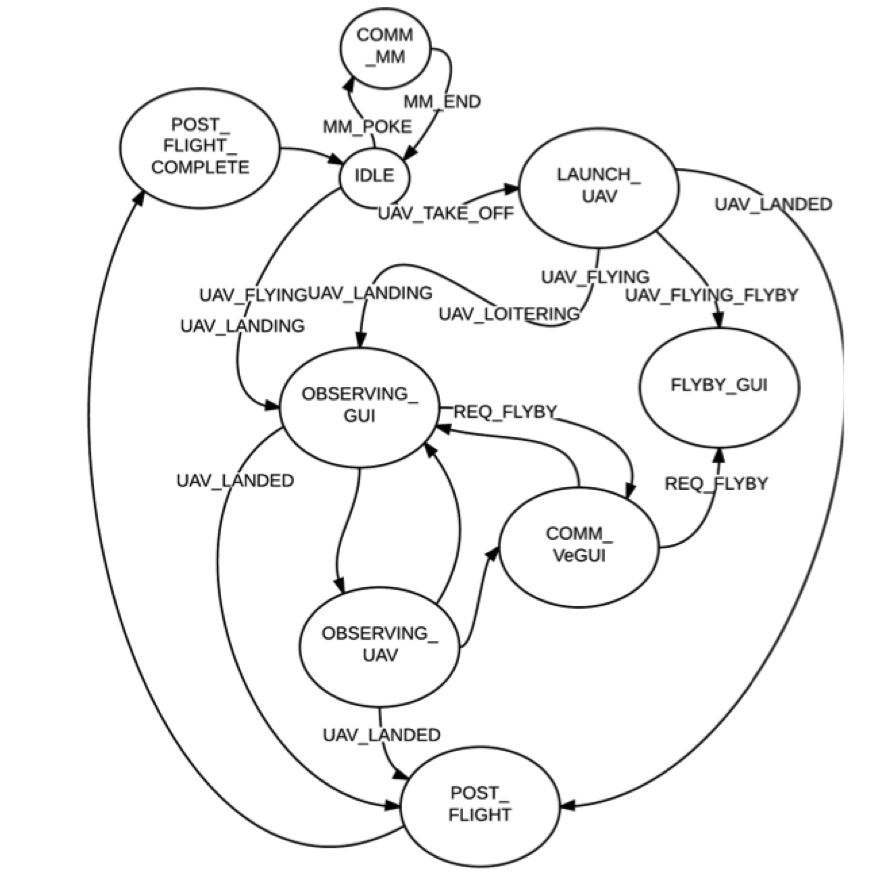
\includegraphics[height=2.4in]{DiRG.png}
\caption{Example actor model from prior work.}
\label{fig:dirg}
\end{figure}
\end{comment}

Actors represent the human decision-makers and autonomous elements of the WiSAR team.  An actor is composed of a set of states $S$, an initial state $s_0$, a set of inputs from the environment $\Sigma_{\rm env}$, a set of inputs from other actors on the team $\Sigma_{\rm team}$, a set of outputs $\Lambda_{\rm out}$, a simple form of memory $\Omega_{\rm men}$, and a transition function that determines the next state from the inputs and memory $\delta$. Formally, we denote an actor as:
\begin{equation}
 	Actor = (S, s_0, \Sigma_{\rm env}, \Sigma_{\rm team}, \Lambda_{\rm out}, \Omega_{\rm mem},\delta)
 \label{eq:actor}
 \end{equation}

 An actor's output has two components: signals to other actors on a team and a {\em duration} parameter that represents the time required for the actor to complete its transition to the next state.  Thus, $\Lambda_{\rm out}=\Sigma_{\rm team} \times \mathbb{N}^+$.
Relative task difficulty is expressed by the duration of the transition.
%The duration represents the relative difficulty of the task(s) associated with the transition.
We justify this by assuming that all tasks are performed at a constant rate, thus more difficult tasks take longer.
 A transition is a relation on the cross product of inputs with outputs where the brackets separate inputs from outputs.
\begin{equation}
 \delta:[S\times\Sigma_{\rm env}\times\Sigma_{\rm team}\times\Omega_{\rm mem}] \times [S\times \Sigma_{\rm team} \times \Omega_{\rm mem}], 
\end{equation} 
 
Given an actor's current state, set of input signals, and memory, it is possible for multiple transitions to be possible.  This occurs because we assume that multiple environment signals or inter-actor signals may be occurring at the same time, which are all perceived by the actor since we assume perception is a parallel operation.  Thus, it is useful to explicitly note the number of transitions that are possible from a given state.   A transition is considered {\em enabled} when all of its input
requirements are met and {\em disabled} otherwise. 

When an actor is in a given state, it is useful to explicitly denote the set of enabled and disabled transitions.  This information enables an estimate of algorithmic workload, where we assume that algorithmic workload is a function of the number of choices available to the actor.  Thus, we allow the current state to give a workload signal
\begin{equation}
	s_0^{\rm work\  sig} = (T_{enabled}, T_{disabled}) : T_{enabled} \cap T_{disabled} = \emptyset
 \label{eq:state}
\end{equation}

Internal variables within an actor are comprised of facts stored by an actor and used in decision making.
%Internal facts stored by an actor and used in decision making take the form of internal variables within an actor.
A good example of this can be seen in the mission manager actor of our simulation. As the search begins, the mission manager receives a number of data items from the parent search, e.g. search area and target description. These items of information need to be communicated separately to different actors, so they must be stored internally in the mean time. 

\section{Directed Team Graph (DiTG)}

A key element of the actors is that inputs to one actor can be outputs from another actor.  We can therefore create a directed graph from actor to actor, with an edge from actor~A to actor~B existing if the output from actor~A is a possible input to actor~B.  We call this graph a {\em Directed Team Graph} (DiTG); Figure~\ref{fig:ditg} illustrates the DiTG for the WiSAR team used in this paper.   

Using the fact that multiple resource theory indicates that visual and auditory channels can be perceived in parallel \cite{wickens2002multiple}, it is useful to label the edges in the graph with the {\em channel type} as in Figure~\ref{fig:ditg_detail}.  These labels allow the model-checker to identify when multiple signals are given to a single actor over the same channel.  When this occurs, we expect actor workload to be high.

%We hope to gain
%insight into decreasing the system workload, and possibly combining roles, by
%establishing metrics associated with the system model and model simulation. 
%These metrics can then be used to determine if changes to the model represent a
%decrease in operator workload.

\begin{figure}[h]
\center
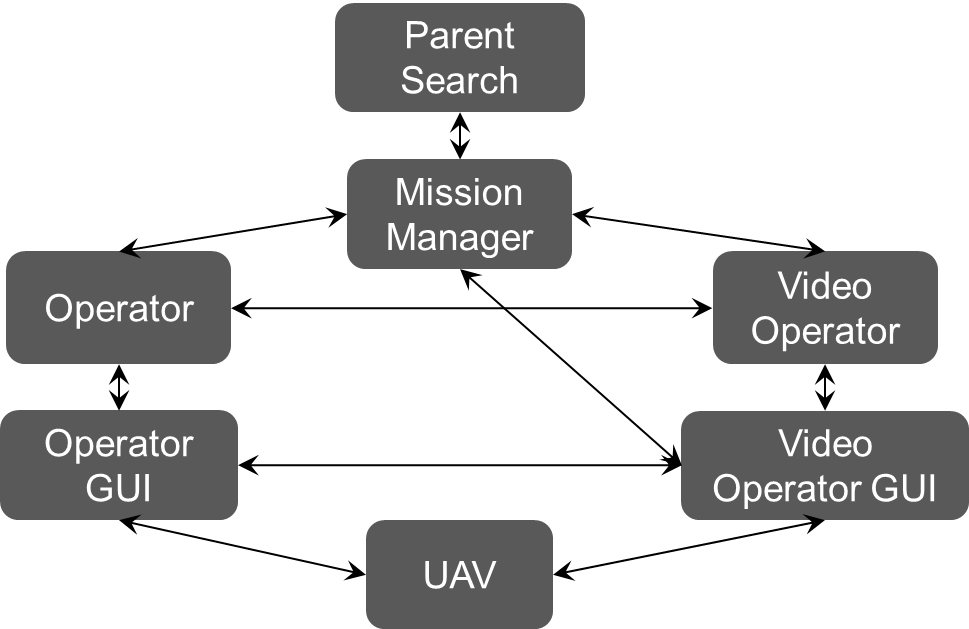
\includegraphics[width=4in]{ditg.png}
\caption{High Level DiTG}
\label{fig:ditg}
\end{figure}

\begin{figure}[h]
\center
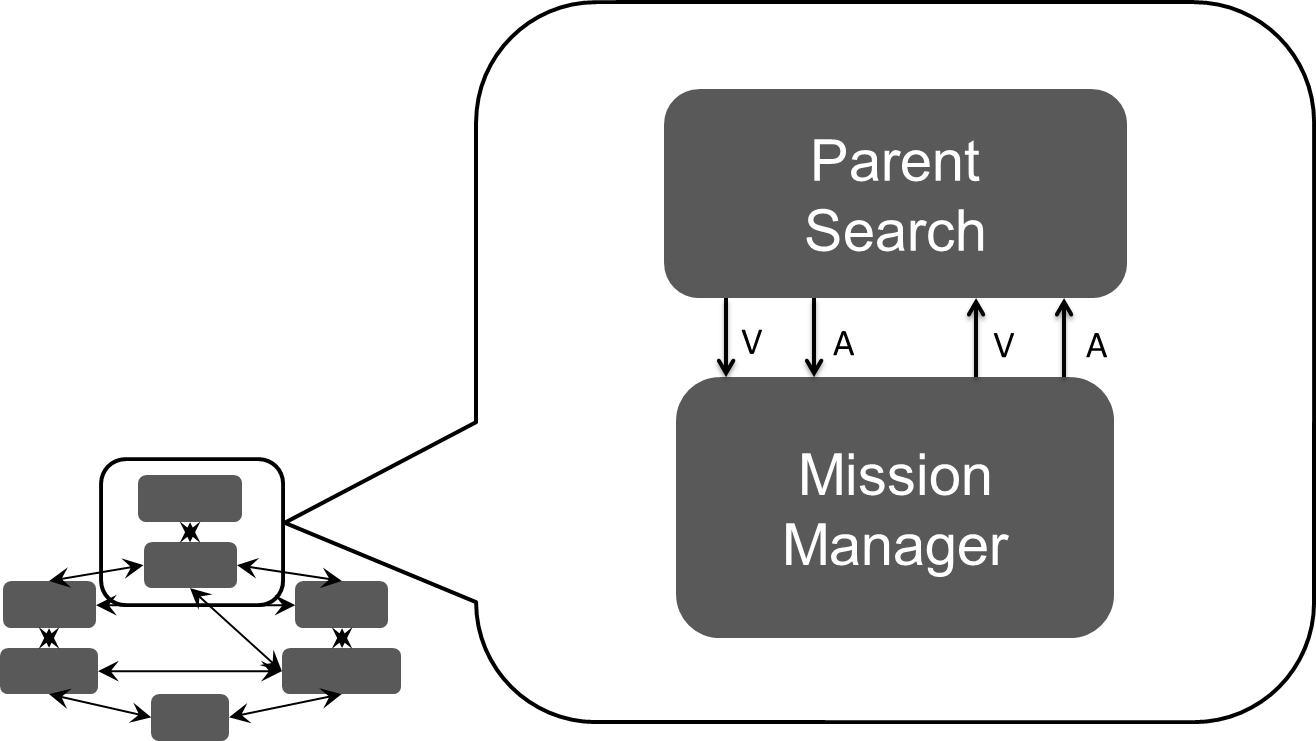
\includegraphics[width=4in]{ditg_detailed.png}
\caption{Detail view of DiTG: V is a Visual channel and A is an Audio channel}
\label{fig:ditg_detail}
\end{figure}

%Formally, the framework is the following mathematical structures:
% \begin{equation}
% 	DiTG = (A, \Phi, \forall a_i \in A~ \exists \Phi_i \subset \Phi)
% \end{equation}

% \begin{equation}
% 	Actor = (S, s_0, s_{current}, \Omega_A, \Sigma_A \subset \Phi, \Lambda_A
% 	\subset \Phi)
 %\label{eq:actor}
 %\end{equation}
%
% \begin{equation}
%	State = (T_{enabled}, T_{disabled}) : T_{enabled} \cap T_{disabled} = \emptyset
% \label{eq:state}
%\end{equation}
%
%\begin{equation}
%\begin{split}
%	Transition = (\Omega_{input} \subset \Omega_A, \Sigma_{input} \subset \Sigma_A,\\
%	\Omega_{value}^{input}, \Sigma_{value}^{input} \\
%	\Omega_{output} \subset \Omega_A, \Lambda_{output} \subset \Lambda_A, \\
%	\Omega_{value}^{output}, \Lambda_{value}^{output}, duration)
% \label{eq:transition}
% \end{split}
%\end{equation}

%\begin{equation}
%\begin{split}
%Channel (\phi) = (type \in (visual, audio), \\
%value \in (null, *), 
% a_i^{source}, a_j^{target}) : i \neq j
% \label{eq:channel}
% \end{split}
%\end{equation}
%
%\begin{equation}
%Declarative Memory(\omega) = value \in (null, *)
%\end{equation}


%\noindent where $A$ is a set of actors, $S$ a set of
%states, $T$ a set of transitions, $\Phi$ a set of channels, $\Omega$ a set of
%declarative memory, $\Sigma$ a set of input channels, and $\Lambda$ a set of
%output channels.

We represent a system as a DiTG, a collection of
actors connected to one another by a set of channels.  Whenever the state of the
system changes, an actor will petition from its current state, a list of enabled
transitions thus defining what decisions can be made.  The actor may then
activate one of these transitions.  

Since transitions from one state to another take time, as encoded in the {\em Duration} element of the output, it is useful to label transitions as either {\em active} or {\em fired}. Transitions in the actor model are labeled as {\em enabled} and {\em disabled}. When we consider the workload of an actor as part of the overall team, workload depends on what is going on with other team members, so we add the active and fired labels in order to determine when an enabled transition (meaning a possible choice available to an actor) is chosen by an actor (making it active) and when the actor completes the work required to enter the next state (the transition fires).  

From an implementation perspective, when a transition becomes active it creates temporary
output values for declarative memory and channels.  These temporary values are
then applied to the actual declarative memory and channel values once the transition fires.

For our model we never explicitly define a single task.  Instead
we define actors, states, and transitions.  Each transition defines its own
perceptual, cognitive, response, and declarative resources \cite{salvucci2008threaded}, allowing the model to represent multiple possible tasks.\footnote{Grant, Kraus, and Perlis have done exceptional work compiling formal approaches
to teamwork. While the formalisms are not explicit in our modeling, our informed
modelers apply these approaches. For example, joint intentions are represented
in actors containing complement transitions.}  In this way, an actor's state
determines what task(s) are being performed, achieving multi-tasking without
explicitly defining tasks. 

%\subsection{Model Creation}
%To simplify the modeling process and ensure rigorous model creation we
%developed a transition language, similar to a Kripke structure, which allows
%models to be expressed as a list of Actor transitions.  A parser then
%automatically generates the classes required to run the model simulation.
%The transition language uses the following structure.
%\begin{equation}
%\begin{split}
%(s_{current}, [\phi_{input} = value,\ldots], [\omega_{input} = value,\ldots],\\
%duration) \times \\
%(s_{next}, [\phi_{output} =
%value,\ldots], [\omega_{output} = value,\ldots])
%\end{split}
%\end{equation}
%\noindent The language is compiled to a Java program suitable to run standalone
%as a simulation or analyzed by the JPF model checker to create
%workload profiles.


To simplify the modeling process and ensure rigorous model creation we
developed a transition language, similar to a Kripke structure,\footnote{Since our purpose behind building a model was to allow us to examine workload we decided against using standard model checkers such as Spin since they did not provide the same level of flexibility that we obtained via java and JPF.}  which allows
models to be expressed as a list of Actor transitions.  A parser then
automatically generates the classes required to run the model simulation.
The transition language uses the following structure.
\begin{equation}
\begin{split}
(s_{current}, [\phi_{input} = value,\ldots], [\omega_{input} = value,\ldots],\\
duration) \times \\
(s_{next}, [\phi_{output} =
value,\ldots], [\omega_{output} = value,\ldots])
\end{split}
\end{equation}
\noindent The language is compiled to a Java program suitable to run standalone
as a simulation or analyzed by the JPF model checker to create
workload profiles.

\section{Workload Metrics}

We are now in a position to combine the three categories of workload (cognitive, algorithmic, and temporal) with the formal model of the actors and team to generate a set of workload metrics.  Because the categories include many possible measurements that are beyond the scope of this paper, we use labels for the workload metrics that are slightly different from the workload categories.  As shown in Figure~\ref{fig:WorkloadMetrics}, cognitive workload or resource workload as it is termed in this work, is measured using metrics under the {\em resource} workload label, algorithmic under {\em decision}, and temporal workload is labeled the same. 


\begin{figure}[h]
\center
\setlength{\abovecaptionskip}{1mm}
\setlength{\belowcaptionskip}{1mm}
\setlength{\textfloatsep}{1mm}
\setlength{\floatsep}{1mm}
\scalebox{.8}{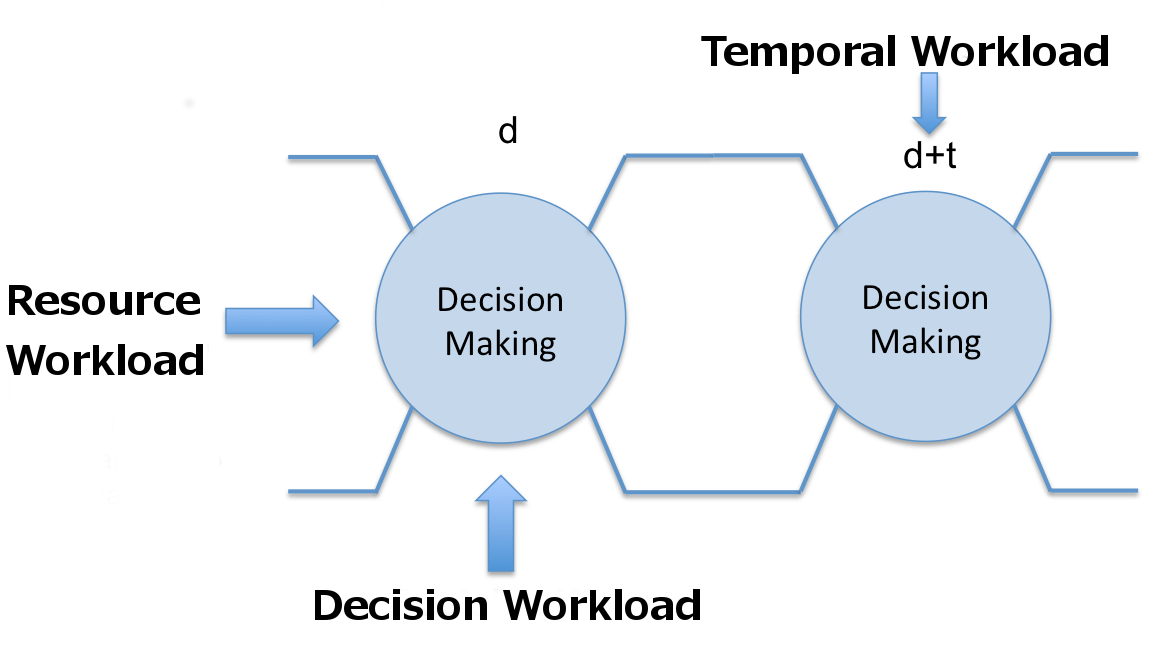
\includegraphics[height=2.5in]{WorkloadMetrics.png}}
\caption{Workload in the model.}
\label{fig:WorkloadMetrics}
\end{figure}

Resource workload is separated into both inter-actor communication and actor
memory load. Decision workload can be broken down into timing, algorithm complexity, and complexity of the solution. Temporal workload includes operations tempo, arrival rate, and response time.

Java Pathfinder (JPF) is a tool used to explore all points of nondeterminism.
%find all possible paths represented in Java source code. 
It does this by compiling the source code as a JPF binary and
running it in a virtual machine.
Sections of the program are then dynamically altered 

The virtual machine can dynamically alter sections of the program and concurrently generate and run copies of the program
based off of these changes. This allows us to include alterable values in our
model and simulate an array of different actors without the need to modify the
model.

We have set up a JPF listener to record workload. A JPF listener is a tool that
follows the Listener Design Pattern and acts in the expected fashion. We have
focused our listeners on three pieces of the model: the active inputs, enabled
transitions, and the time taken to perform a transition. We then use these
pieces of the model to represent resource, decision, and temporal workload respectively.

\section{Results}

In the interest of consolidating operators it is critical to find an accurate measurement that detects situations that exceed the capacity of a given human. One way to detect this is by building a map of each actor's workload as a function of time. JPF explores all possible paths the model can take and returns the ones that violate the model's criteria. By augmenting our model with the workload metrics we can identify all possible areas of high workload. 

We propose three levels of increasing validity for evaluating the approach in the paper.  The first level, the one used in this paper, is to check for {\em consistency}.  We say that the approach is {\em consistent} if the workload peaks, valleys, and trends match what we know about a small set of given situations; in other words, the approach is consistent if it matches our expectations on tasks that we know a lot about.  

The second level, which is an area for future work, is to check for {\em sensitivity}.  We say that  the approach is sufficiently {\em sensitive} if we can use JPF to find new scenarios that have very high or very low workloads, and we can then generate a satisfactory explanation for the levels of workload by evaluating the new scenarios.  The third level, another area of future work, is to {\em substantiate} workload levels using experiments with human participants by comparing the perceived workload of humans with those predicted by the model.

In this paper, we restrict attention to finding areas of high and low workload, and then checking these areas for consistency.  We evaluated consistency using two scenarios.  The first is when the Video Operator was able to identify the target during a flight without any complications occurring (see Figure~\ref{fig:WorkloadSim1}). As the workload measure currently does not have units, the plots are normalized in each category. For the first 40 time steps everything behaves as expected with low to moderate workload. An initial workload bump occurs as actors exchange information necessary to start a search.   At time step forty we see a dramatic deviation from the norm. This deviation is a result of constant information passing between the GUIs and the operators
making it only
%. Since there is a constant passing of data between the machinery and the operators, it is only
 logical that the workload would increase substantially.

\begin{figure}[h]
\center
\setlength{\abovecaptionskip}{1mm}
\setlength{\belowcaptionskip}{1mm}
\setlength{\textfloatsep}{1mm}
\setlength{\floatsep}{1mm}
\scalebox{.9}{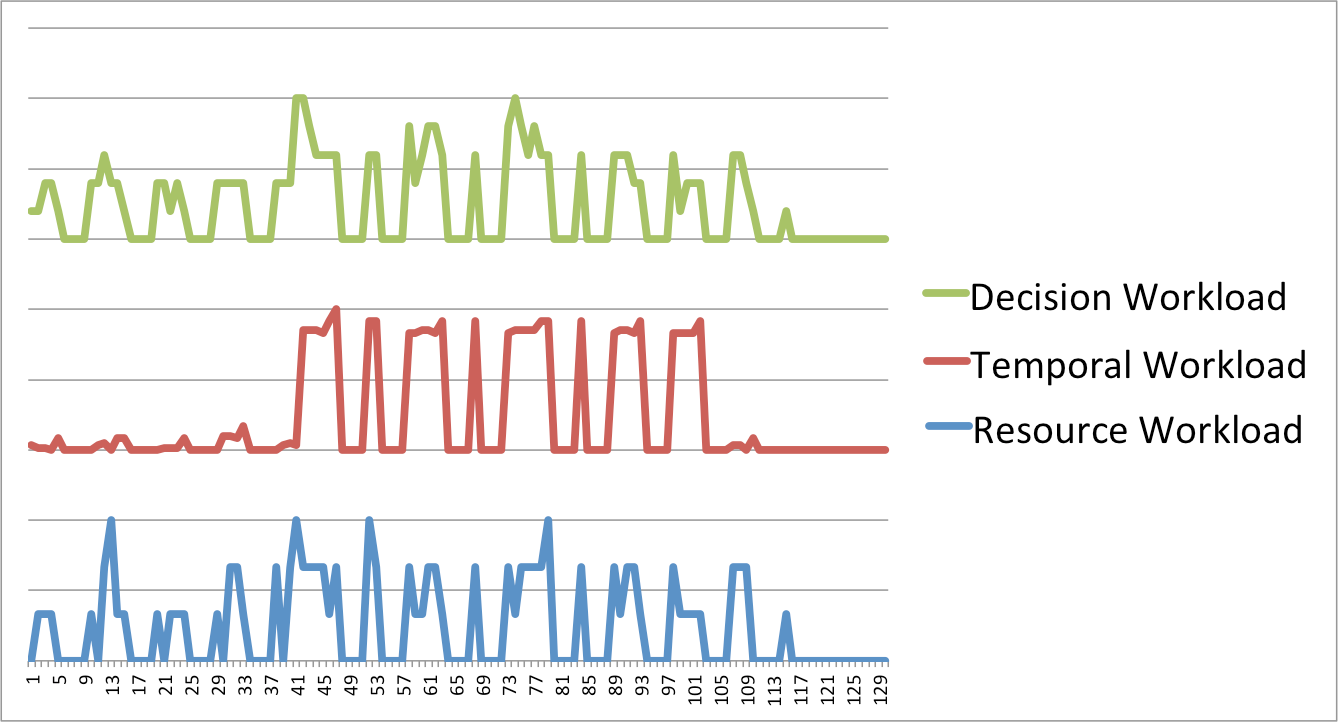
\includegraphics[height=2in]{WorkloadTargetSightingLabeled.png}}
\caption{Workload over an uneventful flight.}
\label{fig:WorkloadSim1}
\end{figure}

The second simulation is a scenario where after a short period of flight the battery rapidly fails. In this particular situation, the operator was unable to respond quickly enough to land the UAV before it crashed (see Figure~\ref{fig:WorkloadSim2}). There is an immediate spike in the temporal workload (middle plot), but surprisingly, the workload then decreases back to normal levels in just five time steps.
The second spike revealed an unexpected fluctuation workload leading us to reexamine how information was reported. We found that there was an error in the simulator that has since been repaired.
%The second spike indicates an unexpected fluctuation in options among one of the actors, which will have to be investigated further to verify if this is an accurate response or if a flaw in the model had slipped past the verification stage of development.
Finally, as would be expected, when the UAV crashed there was a small spike in the workload before everything came to a halt. 

\begin{figure}[h]
\center
\setlength{\abovecaptionskip}{1mm}
\setlength{\belowcaptionskip}{1mm}
\setlength{\textfloatsep}{1mm}
\setlength{\floatsep}{1mm}
\scalebox{.75}{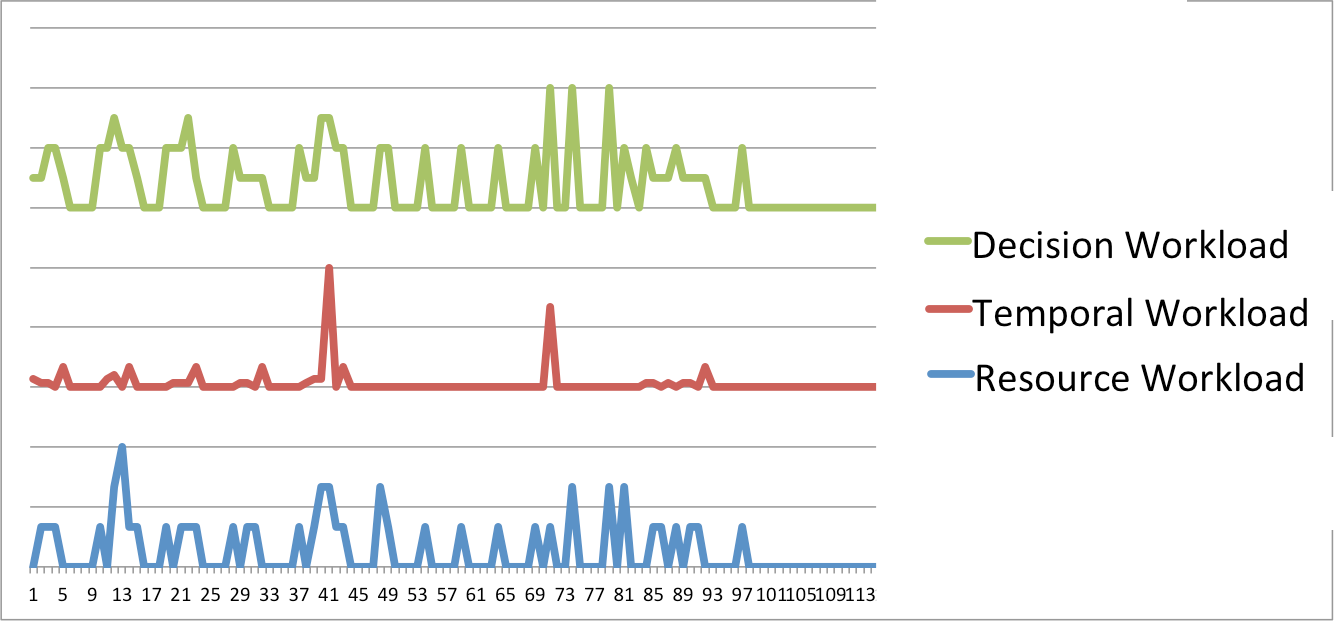
\includegraphics[height=2in]{WorkloadCrashedLabeled.png}}
\caption{Emergency battery failure simulation}
\label{fig:WorkloadSim2}
\end{figure}

\section{Related Work}

This work is an extension of previous work which focused on modeling human
machine systems, specifically WiSAR.  This work extends this model to
incorporate the measurement of workload~\cite{gledhill2013modelinguas}.

Multiple resource theory plays a key role in how we are measuring workload~\cite{wickens2002multiple}. The multiple resource model defines four categorical dimensions that
account for variations in human task performance.  A task can be represented as a vector of these dimensions.  Tasks interfere when they share resource dimensions.  Using these vectors, Wickens defined a basic workload measure consisting of the task difficulty (0,1,2) and the number of shared dimensions.  Using this metric it is possible to predict task interference by looking at tasks which use the same resource dimensions.  Our model differs in that we do not explicitly define tasks, instead we use Actor state transitions which may imply any number of concurrent tasks.  The transition then informs us of which resources are being used and for how long.  

Threaded cognition theory states that humans can perform
multiple concurrent tasks that do not require executive processes~\cite{salvucci2008threaded}.  By making a
broad list of resource assumptions about humans, threaded cognition is able to
detect the resource conflicts of multiple concurrent tasks.  Our model differs from
threaded cognition theory in that it does not allow learning nor does our model distinguish
between perceptual and motor resources. In almost all other aspects our model behaves in a similar fashion.

Related work on temporal workload has attempted to predict the number of UAVs an operator can
control, otherwise known as {\em fan-out}~\cite{cummings2007predicting,OlsenWood2004,CrandallEtAl2005}.  This work used queuing theory
to model how a human responds in a time sensitive multi-task environment.  Queuing theory is helpful in determining the temporal effects of task performance by measuring the difference between when a task was received and when it was executed.  Actors can only perform a single transition at a time, similar to queuing theory, but it is possible for each state to take input from multiple concurrent tasks which differs from standard models of queuing theory.

ACT-R is a cognitive architecture which attempts to model human cognition and
has been successful in human-computer interaction applications~\cite{anderson2004integrated,lebiere2013cognitive}.  The
framework for this architecture consists of modules, buffers, and a pattern-matcher which in many ways are very similar to our own framework.  The major
difference is that ACT-R includes higher levels of modeling detail, such as memory access
time, task learning, and motor vs perceptual resource differences.  Our model exists at a higher level of abstraction.

Complementary work has been done using Brahms.
%Brahms is a powerful language that allows for more detail than our research required.
Brahms is a powerful language that allows for far more detail than we found our research required.
In addition at the time we started developing our model Brahms lacked some of the tools we needed for extracting workload data from the model. Because of this we found that Java in conjunction with JPF made a better match for our needs.

\section{Summary and Future Work}

This paper proposes a model-checking approach to analyzing human workload in an UAS.  Humans and other autonomous actors are modeled as modified Moore machines, yielding a directed graph representing team communication.  Workload categories are distilled from the literature, and the models of the actors and team are augmented so that specific workload metrics can be obtained using model-checking.  Preliminary analysis demonstrates a weak level of validity, namely, that the temporal workload profile is consistent with expected behavior for a set of well-understood situations.  For these scenarios, inter-actor communication is a primary cause of spikes in workload. 

A sensitivity study, followed by an experiment with real human users is needed to understand and justify the workload measures. Once we have verified that our system analyzes workload correctly, it will be useful to design a GUI optimized to managing workload and to formulate a generalized model that will have application to other human-machine systems.


% use section* for acknowledgement
% use section* for acknowledgement
\section*{Acknowledgment}
% optional entry into table of contents (if used)
% \addcontentsline{toc}{section}{Acknowledgment}
The authors would like to thank the NSF IUCRC Center for Unmanned Aerial Systems, and the participating industries and labs, for funding the work.
\chapter{XML Modeling Extension}

Modeling complex human-machine systems is a very difficult and time-consuming task.  This is evidenced by the shear number of modeling approaches to systems involving humans (ACT-R, Soar, DIARC, Brahms, EOFM), the panel ``Modeling Hurts'' at the upcoming AAAI workshop on Formal Methods in Human-Machine Systems, and our own experiences in generating the UE-WiSAR models.  By constructing the MAF Modeling Interface as a set of Java interfaces and abstract classes it meant that the framework was almost entirely extensible in any direction.  We found this very refreshing during the first few development iterations of the framework and model.  We quickly began creating Actors, sub-Actors, Events, States, and Transitions.  Eventually as our model grew in size and complexity the freedom of the Java language became a dual edged sword.  Our model was full of implicit declarations, inconsistencies, duplicated code, and anonymous methods; unbound functions with access to local scope which can be declared in-line which can make debugging more difficult.  It became extremely difficult to maintain the model let alone add to it.  More importantly, it became almost impossible to know if the models were valid and error-free.  This also made it difficult to rely on the metrics we were gathering as each Actor and Transition could implement metric reporting differently.  This chapter discusses an approach to creating MAF models which reduce these problems.

\section{Modeling Approach}

One approach for improving modeling efficiency is to create GUIs which help the user visualize the model in a way which allows them to more easily understand and make changes to the model.  An example of this is the Brahms Composer~\cite{seah2005multi} which allows the user to create models on the GUI and to visualize the model in different ways.  Another simpler approach is to use a language structure which is human readable and facilitates the creation of an accurate mental model.  An example of this is EOFM~\cite{bolton2009enhanced} which uses an XML structure which can be visualized as a tree graph.  The last approach we will mention is the use of design patterns and object oriented principles to build models which do not exhibit these problems.  The downside to this approach is it requires expert Java programming skills to build error-free models.

While others have successfully taken the third approach, for this thesis we chose to take an approach similar to that of EOFM by constructing an XML structure which represents a labeled state transition system.  Unlike EOFM the XML structure is not the main modeling language.  The XML structure represents a subset of the MAF language which is represented by the underlying Java objects which implement the MAF Modeling Interface.  We chose this approach for several reasons:  XML is commonly used for modeling and other similar tasks~\cite{bolton2009enhanced}, it is simple to work with in Java, it is human readable, and it is structured.  This gave us confidence that we would be able to represent any model in XML, perform validation on the model, and then convert the model into Java.  We also chose this approach because the XML is semantically constrained to the structure we define.  The modeler needs only a basic understanding of XML structures and the defined modeling semantics to implement a model.  Another reason for this approach was that it matches the MAF design.  MAF represents a top down approach to abstraction, meaning that the top level Actors, States, Transitions, and Channels are very abstract.  Each subsequent layer removes a portion of that abstraction.  The XML modeling extension adds constraints to the top level Modeling Interface which are designed to remove unwanted abstraction from the modeling language itself.  In this case that abstraction was in the form of unnecessary modeling capabilities.

\section{XML Structure}

We defined the following XML structure to represent the LSTS which is sent to the Simulator.  

The root node is the {\em \textless team\textgreater} element which consists of the {\em name} attribute and three child elements: {\em \textless channels\textgreater}, {\em \textless actors\textgreater}, and {\em \textless events\textgreater}.

\begin{spacing}{.5}
\lstinputlisting[language=XML]{xml_team.xml}
\end{spacing}

\subsection{Channels}

The {\em \textless <channels\textgreater} element represents the DiTG and is comprised of any number of {\em \textless channel\textgreater} elements.  Each {\em \textless channel\textgreater} element represents a single uni-directional communication channel between a source Actor and a target Actor with attributes for the name, type, source, target, and optional dataType.  This is the only location in the XML that defines channels.  Every other {\em \textless channel\textgreater} element references one of these channels by using the channel name as its value.

\begin{spacing}{.5}
\lstinputlisting[language=XML]{xml_channels.xml}
\end{spacing}

\subsection{Actors}

The {\em \textless actors\textgreater} element represents the DiRGs contained in the model and is comprised of one or more {\em \textless actor\textgreater} elements.  Each {\em \textless actor\textgreater} has a {\em name} attribute, which must be unique, and a {\em showMetrics} attribute and is made up of several child elements.  The {\em \textless inputchannels\textgreater} and {\em \textless outputchannels\textgreater} elements are placed here to validate the DiTG.  The {\em actor} may have 0 or more {\em memory} elements which represent declarative memory used internally as part of the labeled state transitions.  The {\em \textless actor\textgreater} contains a list of 1 or more {\em \textless state\textgreater} elements inside of the {\em \textless states\textgreater} element.  Additionally the {\em \textless actor\textgreater} element must contain a single {\em \textless startState\textgreater} element with a value that matches the name attribute of one of the {\em \textless states\textgreater} child elements.

\begin{spacing}{.5}
\lstinputlisting[language=XML]{xml_actors.xml}
\end{spacing}


\subsection{States and Transitions}

The {\em \textless state\textgreater} element represents the `State' in the LSTS.  Each {\em \textless state\textgreater} element has a {\em name} attribute, which must be unique to the parent {\em \textless actor\textgreater} element, and a {\em load} attribute with a value of 0-4, we will discuss state load in the next chapter.  The {\em \textless state\textgreater} element also contains 0 or more {\em \textless transition\textgreater} child elements .  If no {\em \textless transition\textgreater} child elements are specified then it is an end state.  

The {\em \textless transition\textgreater} element represents the `Transition' in the LSTS and is composed of {\em durationMin} and {\em durationMax} attributes which are used for the transition duration range.  It also has a {\em priority} attribute which is used to rank a transitions priority with respect to the other state transitions.  Each {\em \textless transition\textgreater} element contains four child elements: {\em \textless description\textgreater}, {\em \textless inputs\textgreater}, {\em \textless outputs\textgreater}, and {\em \textless endState\textgreater}.  

The {\em \textless description\textgreater} element value contains a description of the transition which is meant to help give the modeler insight into what the transition is actually doing.  It is also used in the debug logs to help track down modeling errors.  

The {\em \textless inputs\textgreater} and {\em \textless outputs\textgreater} elements represent the `Label' in the LSTS.  These elements contain 0 or more {\em \textless memory\textgreater} and {\em \textless channel\textgreater} elements.  All {\em \textless inputs\textgreater} element children have a {\em name} attribute, a {\em predicate} attribute, an optional {\em dataType} attribute and a value.  If the child element is a {\em \textless channel\textgreater} then it may optionally declare only the {\em name} attribute and 1 or more {\em \textless layer\textgreater} child elements which declare {\em name}, {\em predicate}, and optional {\em dataType} attributes along with a value.  The {\em \textless channel\textgreater} name must correlate with an {\em \textless actor\textgreater} {\em \textless inputchannels\textgreater} {\em \textless channel\textgreater} value.  The {\em predicate} attribute contains one of six predicate values: equal to, not equal, greater than, less than, greater than or equal, or less than or equal.  The {\em dataType} is one of three options: String, Integer, or Boolean with a default of String.  The value of these child elements is the value which will be compared against the channel or memory value.  

The {\em \textless outputs\textgreater} element is similar to the {\em \textless inputs\textgreater} element except that its children do not specify {\em predicate} or {\em dataType} attributes.  

This structure allows the modeler to use a 2 dimensional labeling system.  The first dimension being the direction of the data flow, input or output.  The second dimension being the source of the data; channel, layer, or memory.  This allows the LSTS to be very flexible while using a relatively simple syntax.  We should also point out that the transition {\em \textless inputs\textgreater} element contains the following propositional logic: $(Child_{1} \bigwedge Child_{2} \bigwedge \ldots \bigwedge Child_{n})$ which forces the modeler to create a new {\em \textless transition\textgreater} element for each label.

The value of the{\em \textless endState\textgreater} element contains the name of the Actors ending state if this transition were applied.  This value cannot be empty and must match an existing {\em \textless state> name}.

\begin{spacing}{.5}
\lstinputlisting[language=XML]{xml_state_transition.xml}
\end{spacing}


\subsection{Events}

The {\em \textless events\textgreater} element contains a child {\em \textless event\textgreater} element for each unique type of event the system can experience.  The {\em \textless event\textgreater} has a {\em name} attribute, must be unique, and a {\em count} attribute which determines how many times the Simulator will fire the event.  Each {\em \textless event\textgreater} element defines a single {\em \textless transition\textgreater} element which differs from the previously mentioned transition element in that it does not define duration, priority, or an end state.

\begin{spacing}{.5}
\lstinputlisting[language=XML]{xml_events.xml}
\end{spacing}

\section{XML Model Parser}

With the XML structure defined we then moved onto parsing the XML.  See figure~\ref{fig:xml_model_extension}.  To accomplish this we created a Java class named XMLModelParser.  This class performed two main functions.  The first was to create the necessary Java objects and the second was to perform basic error checking on the model.  

The XMLModelParser works by first loading the XML model into an XML object.  This allows us to search the XML structure for specific elements and attributes.  The structure of the XML model facilitates the parsing effort since each child element is also a child object.  The first object which is created is the Team.  Next the DiTG is added to the team by creating ComChannel objects for each channel.  The Actor parsing is the most complex.  Each actor element defines its own DiTG, memory, states, transitions, and labels.  One of the challenges with the Actor parsing was ensuring that the Java objects were constructed in an order which allowed them to link properly.

\begin{figure}[h]
\begin{center}
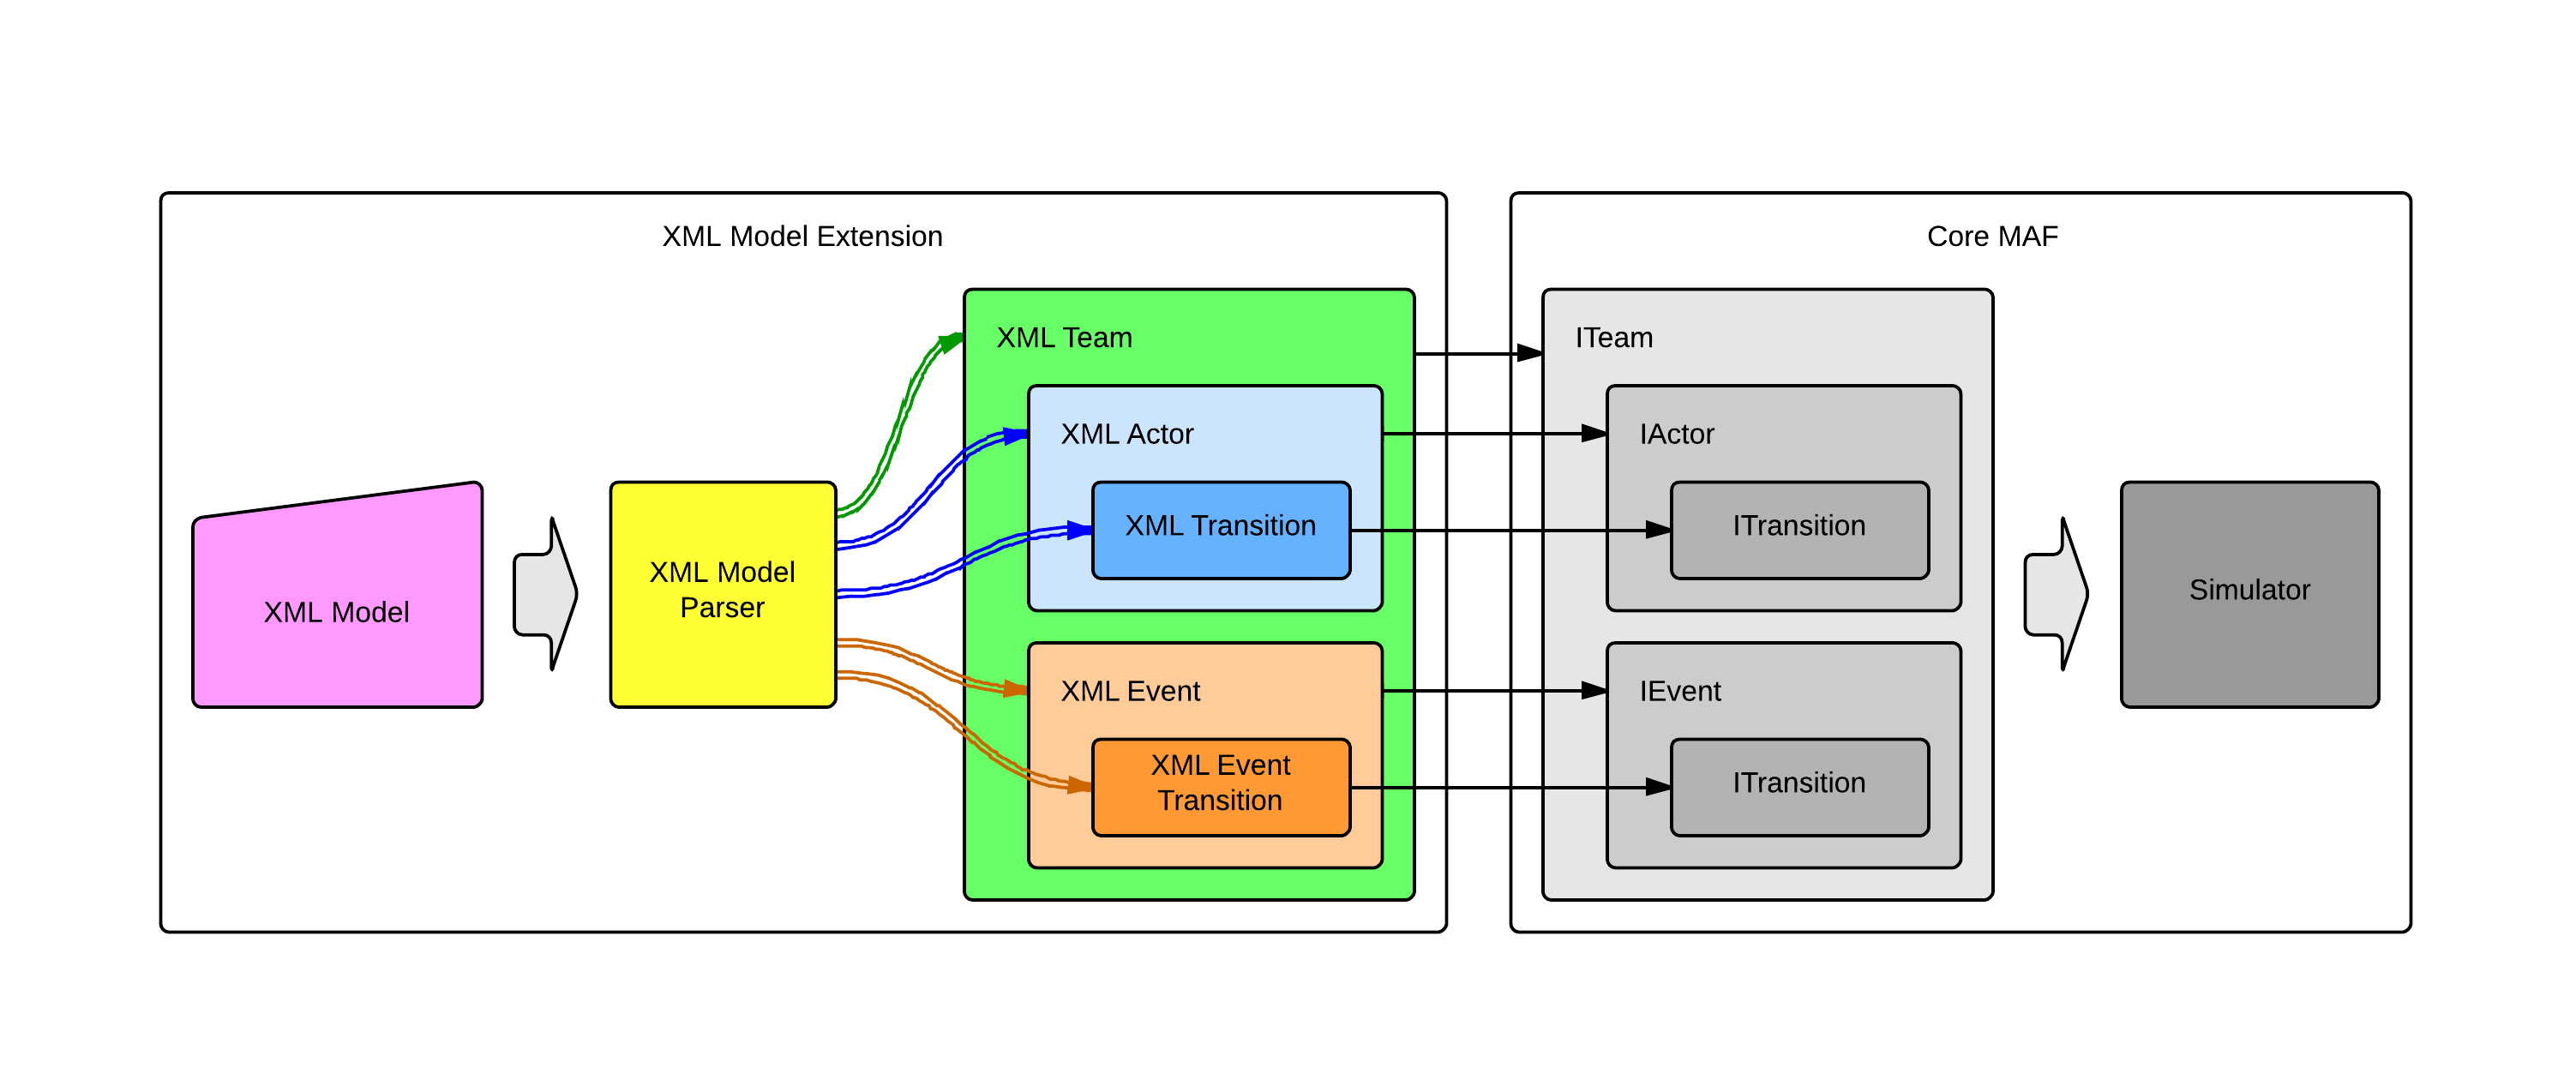
\includegraphics[width=6in]{xml_model_extension.png}
\caption{XML Model Extension Breakdown}
\label{fig:xml_model_extension}
\end{center}
\end{figure}

\subsection{Attaching to the Simulator}

To pass a valid LSTS to the Simulator the XMLModelParser must construct Java classes which implement the MAF Modeling Interface.  To accomplish this we created a set of generic XML classes, each class implements a specific portion of the Modeling Interface such as the ITransition or IActor interfaces.  These interfaces allow the Simulator to query and execute transitions on the LSTS.  The list of XML classes includes the XMLTeam, XMLActor, XMLTransition, XMLEvent, XMLEventTransition and other helper classes.  A link to the source code can be found in appendix~\ref{code}.  Each of these generic XML classes lies separate from the core simulation code.  This means that the addition of the XML parser does not prevent the use of custom Actors or Transition classes, use of a different model parser, or extension of our existing XML parser.  In fact our XML model extension is meant to be expanded to handle a more robust set of models.   As we developed a model using this XMLModelParser we had several occasions to extend its capabilities which we discuss later.  Unsurprisingly it was not difficult to extend the XML to accommodate the changes, often requiring less than 100 lines of code (not including changes to the model XML).

\subsection{Validation}

One of the most time consuming aspects of the modeling process was validating that the model was correct.  By correct we mean that each designed path through the model can and will be traversed when given a specific set of inputs.  In order to ensure that the model was correct we had to manually step through the model simulation paths during construction and check that the correct paths were being taken.  According to commit dates in our github repository we estimate that our initial 5 Actor sample model took three days to create and validate.  The following 12 Actor fully functional model took 34 days to create and validate.  However, the fully functional model only contained $4\times$ the amount of code.  See figure~\ref{fig:time_to_model}.  The discrepancy between the time to model and the model size demonstrates how problematic model validation can become as model complexity increases.

\begin{figure}[h]
\begin{center}
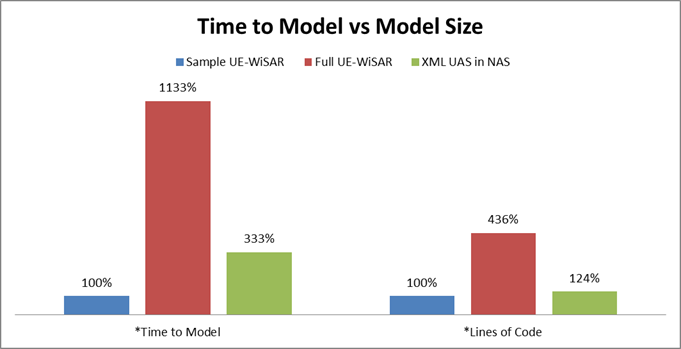
\includegraphics[width=4in]{time_to_model.png}
\caption{*Time to model is an approximation generated by analyzing github commits.  * Lines of code has been adjusted to account for whitespace, comments, and lines with fewer than 5 characters. }
\label{fig:time_to_model}
\end{center}
\end{figure}

We observed several underlying modeling problems which we believe are responsible for the dramatic increase in validation time.  The first problem occurred when the modeler became disoriented while working within the model.  Each time a path branches or the modeler switches branches it becomes more likely that their mental model will diverge from the Java model.  As complexity increases the number of branches and the need to jump between branches also increases.  When this happens mistakes related to a divergent mental model, such as transitioning to the wrong state, forgetting to add a transition, or checking the wrong inputs, begin to appear.  Another problem was a lack of validation tools.  The step-through validation approach essentially meant that only a single modeling error could be found at a time and we had to step through the entire model for each error.  We also observed that modelers are prone to introduce common typing errors into the model which do not get caught by the Java compiler.  

The XML Modeling Extension helps to mitigate these problems in a few different ways.  The XML modeling structure is meant to help offset some of the complexity by presenting the model to the user in a more compact and semantically relevant form.  Java syntax such as class, new, void, etc\ldots are not relevant to the model and do not help the modeler understand the model.  The XML specific syntax however uses a much smaller footprint, additionally the structure itself describes the model in a very concise form which helps the modeler maintain a more accurate mental model which leads to fewer modeling errors.

This extension also helps by introducing a new validation tool.  The need to parse the XML into Java provides a natural location to perform basic error checking on the XML before creating the Java objects which are passed to the Simulator. The simple syntax and structure of the XML makes it much easier to check for user errors in the model.  One of the most common errors we found when creating the UAS integrated into NAS model was missing parameters.  Inside the XMLModelParser if a required portion of XML was not found an error was returned with a description of the problem and where it occurred.  The same was true for an invalid DiTG, duplicate element names, typos, and missing or impossible transitions.  This provided huge time savings when compared with the other alternatives of analyzing output logs or stepping through code with the debugger.

Another benefit introduced with this extension was the generic Java classes.  Each XML component had a single Java implementation.  This guaranteed that similar components would share the same behavior, something which Java interfaces do not provide.  It also meant that bugs in the Java code only needed to be fixed in a single location.

\section{Channel Layers}

While working on this extension it became apparent that our channel design was flawed.  From Threaded Cognition Theory~\cite{salvucci2008threaded} we are aware that an individual can perform multiple concurrent tasks that do not require an executive process.  It does not matter if those concurrent tasks originate from multiple sources or a single source, such as a GUI.  Our previous design restricted channels to a single type of data with no restriction as to what that data type was.  While an arbitrary data type allowed us to pass any amount of data, it made it very difficult to know what was really happening on the communication channel.  What we mean by this is that instead of explicitly defining concurrent tasks we rely on inputs and Actor state to imply that concurrent tasks are being performed.  The arbitrary data type thus prevented a single communication channel from implying multiple concurrent tasks.

To fix this flaw we decided to add layers to our communication channels. See figure~\ref{fig:layers}.  Each channel can have any number of layers.  For example, a visual channel from one person to another has two channels, one which analyzes the face and another which analyzes the body.  Their may be more accurate channel layering for this scenario but these layers satisfy this example.  When communication occurs on this visual channel the recipient can examine as many layers as are needed for the given state.  If the person is in a distracted state then maybe they are not looking at the face layer which may in turn reduce the probability of comprehending the corresponding audio channel.   Another good example where this is useful is in GUIs.  Each item that a GUI represents to the user can be represented as a different layer.  The more layers a GUI presents to a user the more complex it becomes which potentially makes it more difficult for a person to analyze, due to conflicting resources ~\cite{salvucci2008threaded}.

\begin{figure}[h]
\begin{center}
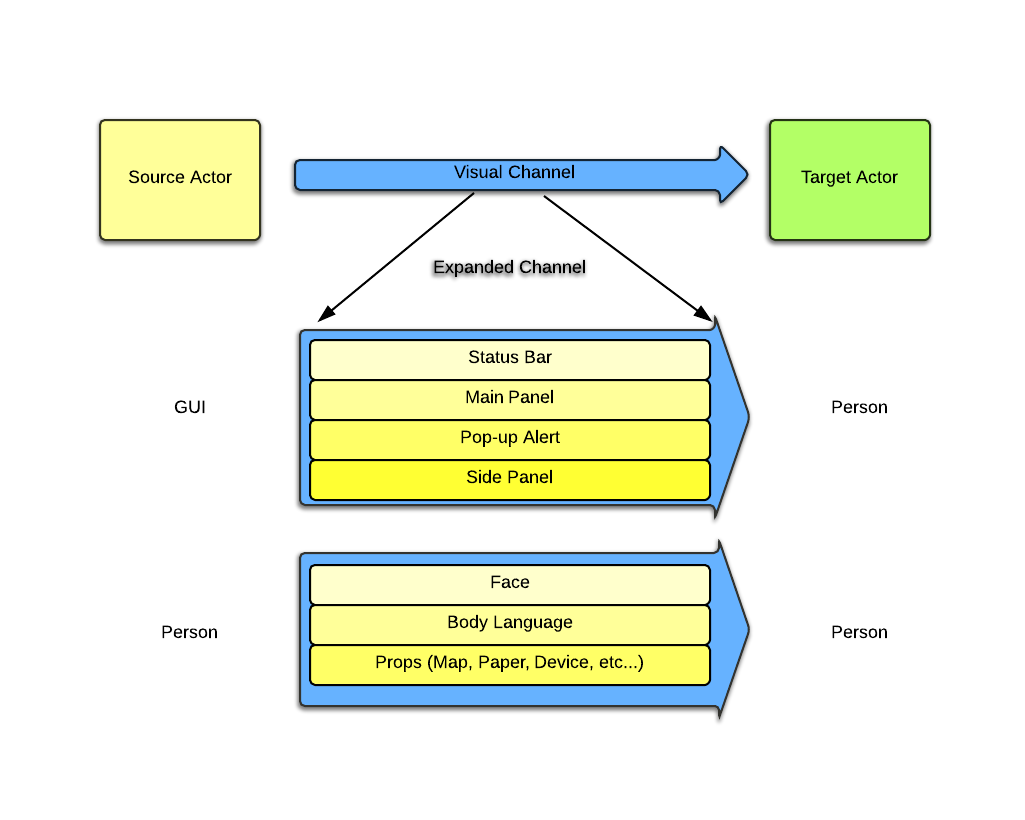
\includegraphics[width=5in]{layers.png}
\caption{Communication Channel Layers}
\label{fig:layers}
\end{center}
\end{figure}

We believe that this concept of channel layers creates a more natural flow of information across the DiTG while aligning MAF with modern human workload theory.  We also have the ability to perform a number of different measurements on the channel layers which, when combined with our other metrics, may prove valuable in obtaining accurate human workload measurements.


\chapter{Metric Improvements}

There are two general approaches for extracting simulation data into meaningful metrics: capture and report all raw data and use post processing to extract the metrics or capture only that data which we know to represent meaningful metrics and ignore the rest.  The first approach is valuable in that the volume of data has the potential to provide many first, second, and third order metrics which are not visible when sampling.  For example other researchers on this project are using trends in the data to help summarize the data at a higher level of abstraction.  Unfortunately the high volume of data also makes it more difficult to find meaningful metrics.  The sample approach simplifies the collection of specific metrics, however, this may make it more difficult to compare multiple metrics if the raw data which connects those metrics was not captured.  This was one of the challenges we faced in obtaining results for chapter 3.

For this thesis we present a mixed data extraction approach.  Figure~\ref{fig:metric_gathering} shows the first in last out metric stack which was used to obtain more accurate metric data from the LSTS hierarchy.  For each time step in the simulation the Simulator will ask the Team for metrics which triggers a chain of metric requests down to the transition level.  When it is time for a component to sample the raw data it will select a sample of the raw data and pass it to its parent.  The parent then selects its own sample data from the available raw data and the sample returned by its child.  This allows the component to perform pre-processing on the raw data which is much easier to accomplish while the data is still within the original context.  It also captures a unified timeline for all of the metrics which helps to tie the metrics together.  We can see this in action by examining the Actor metric stack.  The Actor knows how many input channels he can listen on, his current state, etc\ldots  The Actor does not directly know what transitions are enabled, how many inputs are in those transitions, etc\ldots  Instead of trying to calculate all of this with multiple queries into the state the Actor simply asks the State object for its metrics.  The State then obtains/calculates metric values, obtaining metrics from sub-components if needed, before passing these values back to the Actor.  Once each Actor has returned a set of metrics the Team will then return these metrics, in the form of an array, to the Simulator for storage, post processing, and user display.  Results presented in the next chapter show the value of presenting the metrics in a unified timeline.

\begin{figure}[h]
\begin{center}
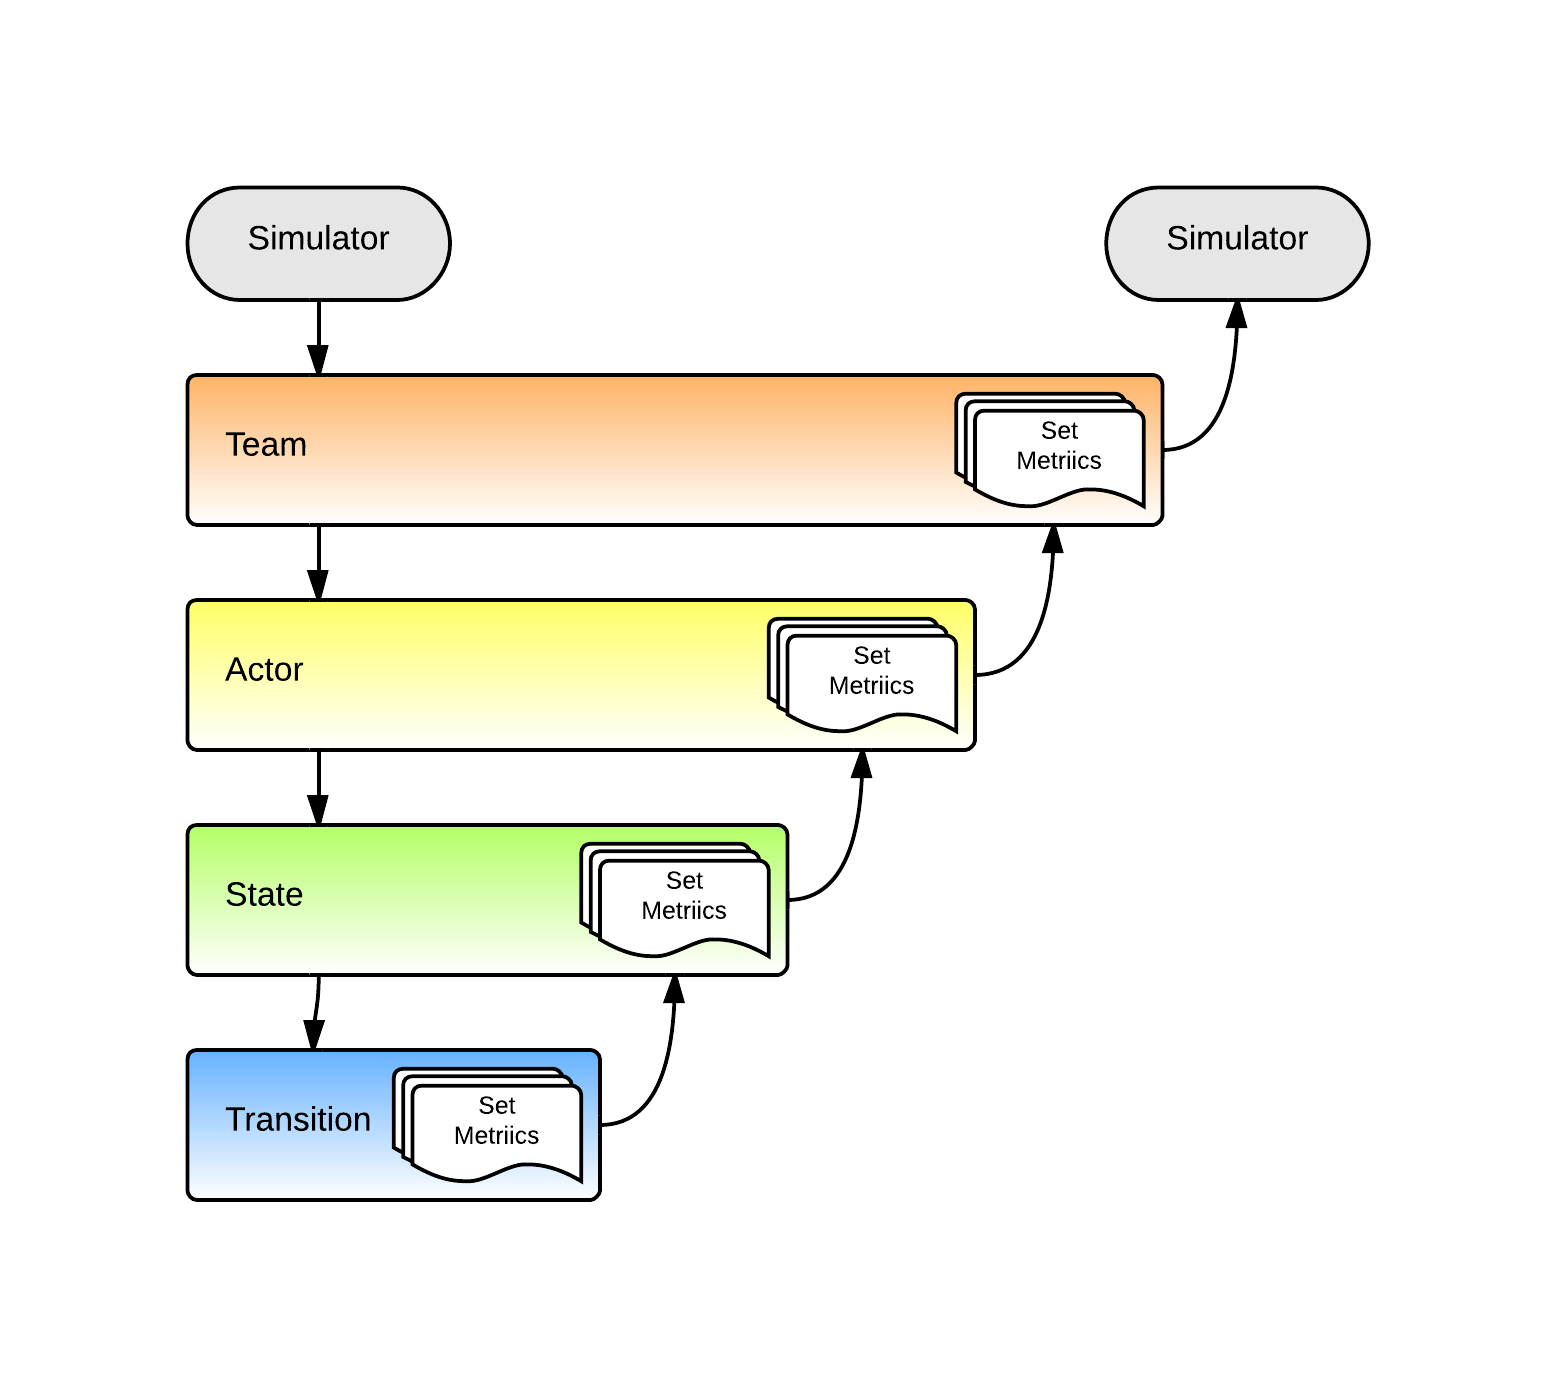
\includegraphics[width=6in]{metric_gathering.png}
\caption{Metric Gathering}
\label{fig:metric_gathering}
\end{center}
\end{figure}

\section{Wickens Workload Model}

Given the ability to extract data from the model hierarchy as described in the previous section, we can translate this data into meaningful metrics.  Since we are interested in metrics which reveal human workload we have chosen to replicate Wickens basic computational model, based on Multiple Resource Theory~\cite{wickens2002multiple}, using data gathered from MAF which we will later use as a baseline comparison against our own metrics.  This Wickens model takes the task difficulty, ranging from 0 to 2 where 0 is automated and 2 is difficult, of two tasks and adds them together.  It then adds the number of dimensional conflicts between the tasks, max of 4, which gives a result between 0 and 8.
	The difficulty with applying this model to our metrics is that we have removed the concept of tasks and replaced it with the notion of state and inputs.  In order to replicate Wickens model we needed a way to represent task difficulty (resource demand) in a similar fashion.  Using transition duration, the longer a task takes the more difficult it is, does not work because it prevents the modeler from placing an Actor into a long running simple task.  Inputs do not work since the data going over a channel does not always reflect resource demand, shown by a humans ability to tune out certain inputs.  Further examination revealed that we had no way to explicitly define an Actors resource demand with MAF.  Wickens model relies on the modelers experience and intuition to set the task difficulty.  Since this is most likely more accurate than any implicitly constructing task difficulty from resource consumption we have also chosen to use this approach which we have labeled as Actor load.
	
\subsection{Actor Load}
Actor load represents an abstraction of the load an Actor is under for any given state.  Similar to Wickens model we will use values from 0-4.  Each Actor state will define its own load.  A load of 0 represents little to no load on the actor.  These are automated or transitional states.  A load of 4 represents simultaneously performing multiple high difficulty tasks.  Any value between 1 and 3 is some combination of task difficulty and the number of tasks being performed.

\subsection{Applying Wickens Computational Model}

By placing Actor Load into the State portion of our models we can now replicate the simple computational model Wickens used in his measurements.  Using the State load as the task difficulty the next step is to find the dimensionality of the resource conflicts.  Since a state represents 1 or more tasks this also presents a challenge.  To best approximate Wickens model we needed metrics which could represent one or more tasks.  We accomplish this by making the assumption that if an Actor has input from multiple sources then multiple tasks are being performed.  It should be noted that we check the input channels for each transition in the current state but only the outputs of the current transition.  With these assumptions we are now ready to calculate dimensional conflicts, Figure~\ref{fig:multipleresourcetheory}.
For the Stage dimension (perception, cognition, response) we check to see if there are multiple sources of input or multiple targets for output.  If there are then we increment the dimensionality.   
For the Modality dimension (Audio, Visual) we check if there are more than a single active channel, input or output, of type audio or visual.  If there is then we increment the dimensionality.  
For the Focus dimension we check if there is more than one source for tactile outputs, if there are then we increment the dimensionality.  We do not check inputs as we have no way of distinguishing if a visual channel has focus.  This may need to be addressed in future work. 
For the Codes dimension (Spacial, Verbal) we check that the total number of audio inputs and outputs is greater than 1 or that the total number of visual inputs, visual outputs, and tactile outputs is greater than 1.  If either value is greater than 1 then we increment the dimensionality.  

By adding the task difficulty (Actor load) and the dimensionality together we obtain an adapted Wickens metric which we can then compare with our own metrics.

\begin{figure}[h]
\begin{center}
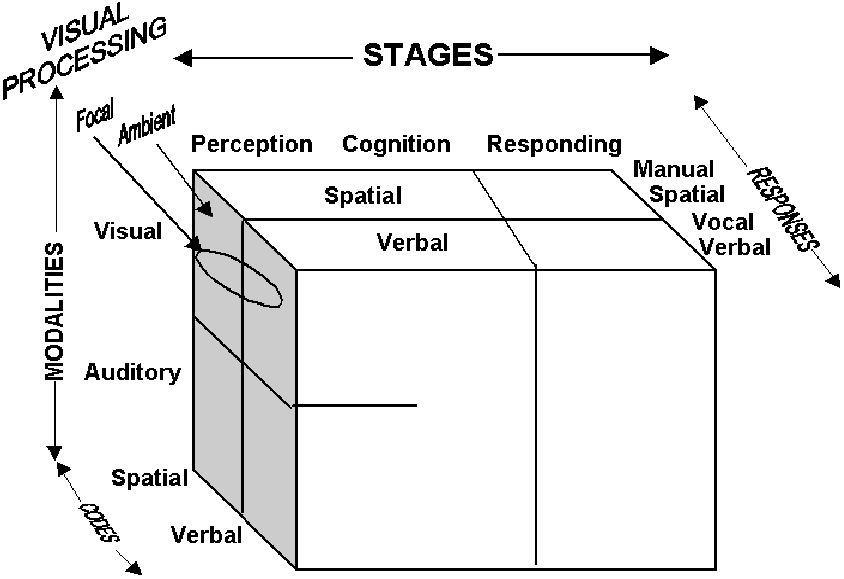
\includegraphics[width=6in]{multresourcetheory.png}
\caption{Multiple Resource Theory Dimensions}
\label{fig:multipleresourcetheory}
\end{center}
\end{figure}

\section{Changes to our Metrics}

As part of the changes to the metric gathering and the addition of a single code base for all Actors, States, and Transitions we implemented the following metric changes which are meant to make the metrics more consistent and more inline with the theory.

For the resource workload category we now generate Actor metrics the following way.  Inputs are gathered from each transition that is part of the current state.  The outputs are collected from the active transition.  We also use the Actor load from the current state.  There are 2 main metrics the channel conflicts and the resource load.  Channel conflicts occur whenever more than one active channel share a type, such as multiple audio channels.  Since we currently only allow visual and audio input for human Actors this value ranges from 0 to 2.  The other metric is the resource load.  This metric attempts to quantify the load being placed on the Actors resources.  We break the resource load into two parts, input and output, the final result being the sum of both parts.  Each part is calculated by adding the number of active channels, number of layers read, number of memory objects read, and the number of active channel types.

For decision workload we have added input complexity and output complexity.  The input complexity is the total number of active inputs plus the number of memory inputs.  The output complexity is the number of output channels plus the number of memory outputs.  While there is overlap between these values and the resource workload metrics we leave it up to future work to analyze this relationship.  We have also modified the duration complexity metric.  Before adding Actor load we relied on the duration complexity to inform us of task difficulty.  We no longer apply the same weight to the durations.  Instead we are now using a logarithmic scale.  By assuming that durations are in seconds we classify any transition under a minute as 0 complexity and move up from there.  Our reasoning for this normalization is two fold.  First it is reasonable to assume that the more time a transition takes the more workload it requires, however, it is also reasonable to assume that there are diminishing returns associated with increasing the workload.


\section{Other Changes}
We also performed additional minor refactors to MAF to facilitate the previously described changes.  As part of this refactoring the connections to JPF were temporarily disabled in order to simplify the debugging process.  The results described in the next chapter were obtained by running the simulator as a stand alone application outside of JPF.  While this does prevent a deeper evaluation of the models state space the core model behavior still remains the same.  Unfortunately it prevented us from collecting the temporal workload metrics from the model.

\chapter{Case Study: UAS operating in the NAS} \label{ch:UASinNAS}

\begin{comment}
According to the integration of civil Unmanned Aerial Systems into the Nation Airspace System roadmap~\cite{nasroadmap} the FAA is working with other government agencies and industry to develop a collaborative UAS modeling and simulation environment to explore key challenges to UAS integration. The near-term modeling goals are to:
\begin{itemize}
  \item Validate current mitigation proposals
  \item Establish a baseline of end-to-end Unmanned Aerial System performance measures
  \item Establish thresholds for safe and efficient introduction of Unmanned Aerial Systems into the National Airspace System
  \item Develop NextGen concepts, including 4-dimensional trajectory utilizing Unmanned Aerial Systems technology
\end{itemize}

We believe that the Model Abstraction Framework accomplishes each of these goals.  The framework is extremely flexible, allowing it to model a large variety of systems at varying and alternating degrees of abstraction, an attribute that is ideal for new designs.  It has the ability to detect critical failures.  It has the ability to examine multiple paths through the model and to randomly perturb the model in different ways to explore these paths.  It also generates human workload metrics that are valuable for setting safety thresholds and analyzing new designs.

The roadmap~\cite{nasroadmap} also identifies several interrelated research challenges:
\begin{itemize}
  \item Effective human-automation interaction (level of autonomy; trust; and mode awareness)
  \item Pilot-centric ground control station design (displays; sensory deficit and remediation; and sterile cockpit)
  \item Display of traffic/airspace information (separation assurance interface)
  \item Predictability and contingency management (lost link status; lost ATC communication; and ATC workload)
  \item Definition of roles and responsibilities (communication flow among crew, ATC, and flight dispatcher)
  \item System-level issues (NAS-wide human performance requirements)
  \item Airspace users� and providers� qualification and training (crew/ATC skill set, training, certification, and currency)
\end{itemize}

The Model Abstraction Framework was specifically designed to model human-automation interaction for UAS.  Our WiSAR model specifically demonstrates predictability and contingency management for each path in the model.  The DiRG allows us to model specific roles and their responsibilities while the DiTG defines communication flow between different roles.  And the workload metrics allow models of human performance to be verified.

Due to the nearly identical nature of the FAA's goals with our own, we have modeled a basic Unmanned Aerial System integrating into the National Airspace System.  Due to our lack of domain knowledge we have had to make a number of assumptions in order to achieve a high level of abstraction.  Despite the high level of abstraction we believe that the results are informative.
\end{comment}

To analyze the workload metrics presented in the previous chapter we chose to perform a case study by modeling the integration of a UAS into the National Airspace System.  First we will describe the scenario that we modeled and the assumptions required to make the model work.  Then we will present an analysis of the workload metrics gathered using the Model Abstraction Framework.

\section{Model Scenario and Assumptions}

Since we would eventually like to correlate these workload metrics with real human workload our goal was to model a UAS that presented high and low workload periods similar to those observed during the WiSAR flight tests.  Such as creating fight plans, monitoring normal flight, handling active alarms, introducing increased autonomy, and handling operator interruptions.  This will allow us to check that the results are generally consistent with a known workload profile.  The model we chose was the integration of a UAS into the National Airspace System.

To help illustrate this model we have created a DiRG that shows the states and data flow for each Actor.  Figure~\ref{fig:uasnasdirg}.  A matching DiTG for the model showing the Actor communication channels can be seen in figure~\ref{fig:uasnasditg}.

An Unmanned Aerial System (UAS) plans to operate within the National Airspace System.  The UAS is composed of a server (UAS Server), an Unmanned Aerial Vehicle Operator (UAV Operator), and an Unmanned Aerial Vehicle (UAV).  The UAV Operator controls the UAS Server through a graphical user interface (UAS GUI) that in turn controls the UAV, as illustrated in the DiTG shown in figure~\ref{fig:uasnasditg}.  The UAV will take off and land at an airport serving both manned and unmanned aerial vehicles.  The UAV Operator is located at this airport and visually monitors the takeoff and landing of the UAV.  UAV state is continuously shown on the UAS GUI.

\begin{figure}[h]
\begin{center}
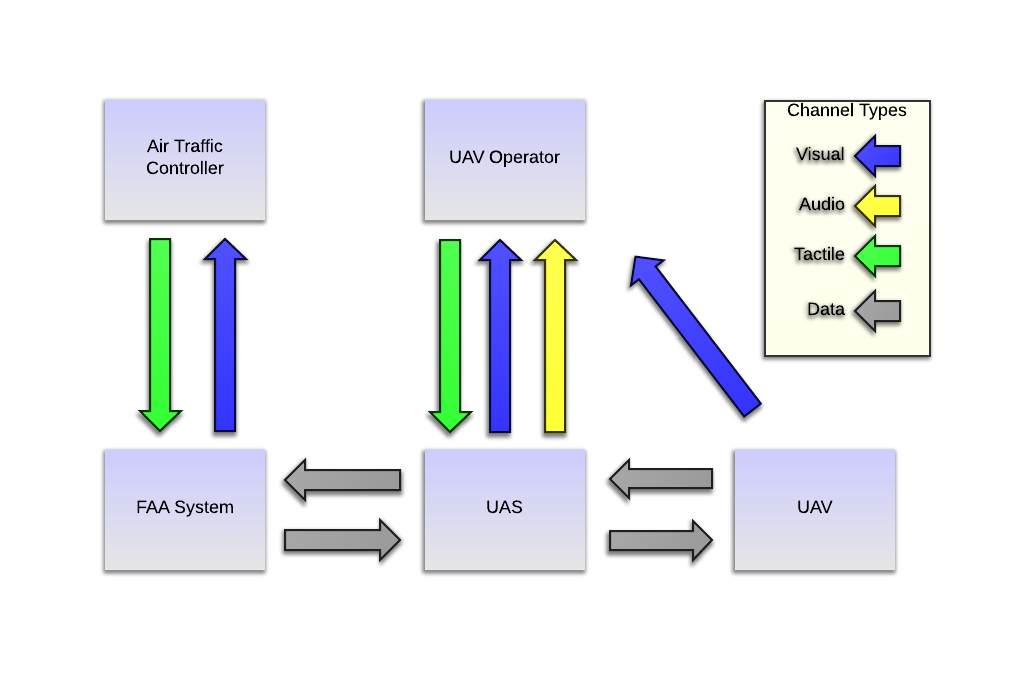
\includegraphics[width=5in]{uasnasditg.png}
\caption{DiTG: UAS integration into the NAS Model}
\label{fig:uasnasditg}
\end{center}
\end{figure}

There is an FAA Server that provides real-time notice to airmen (NOTAM) information.  The UAS Server connects to this server, receives the NOTAMs and displays them on the UAS GUI.  Figure~\ref{fig:uasnasditg}.  The FAA system also allows the UAS Server to file flight plans.  Filed flight plans are automatically checked for simple conflicts such as crossing NOTAMS or duplicate takeoff/landing times.  If there is a conflict the FAA Server flags the flight plan for an Air Traffic Controller (ATC) and displays these requests on an FAA GUI that is monitored by the ATC.  The ATC then approves or denies flight plans, using the FAA GUI, at their leisure.  This approval/denial then becomes available to the UAS Server, which displays it on the UAS GUI as illustrated in the DiRG shown in Figure~\ref{fig:uasnasdirg}.

\begin{figure}[h]
\begin{center}
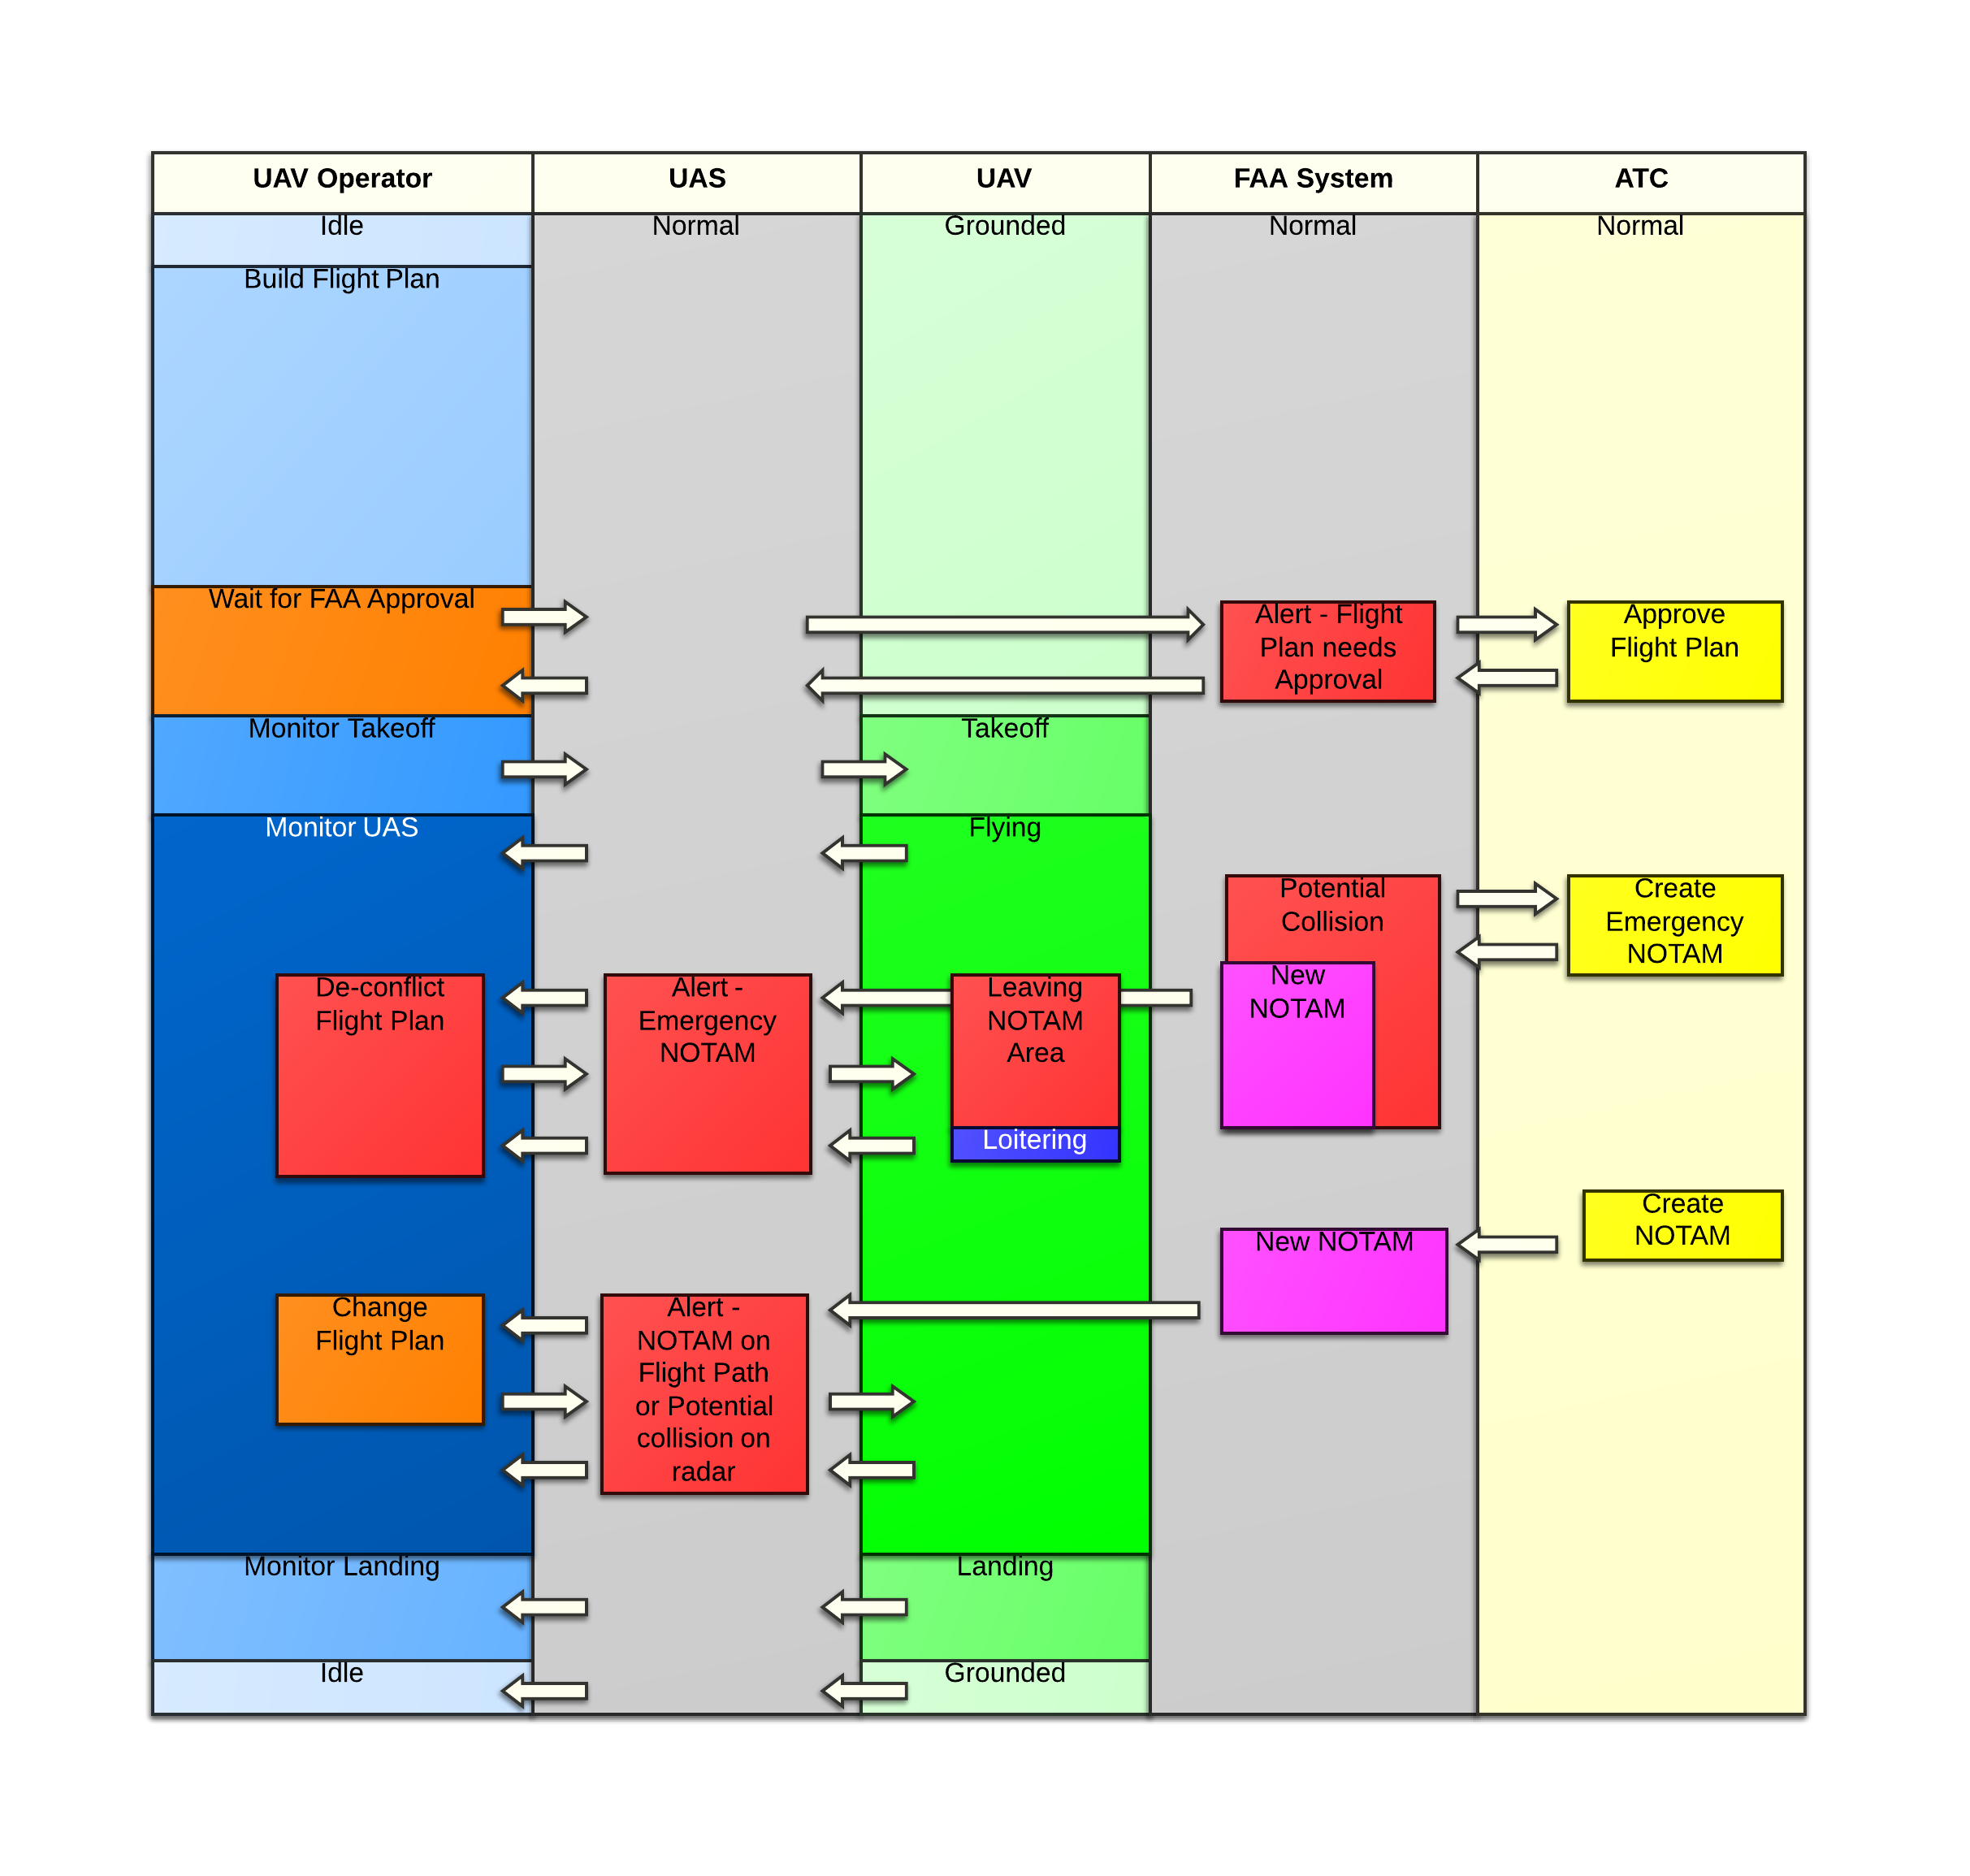
\includegraphics[width=6in]{uasnasdirg.png}
\caption{DiRG: UAS integration into the NAS Model.  Columns represent Actors, column sections represent states, and arrows represent inter Actor data flow.}
\label{fig:uasnasdirg}
\end{center}
\end{figure}

The FAA Server also provides radar information to the ATC through the FAA GUI.  The ATC uses this information to spot potential collisions with UAVs.  If a potential UAV collision is detected the ATC creates an emergency NOTAM in the region of conflict.  This emergency NOTAM is then sent to the UAS Server, which displays the emergency NOTAM on the UAS GUI.  If the UAV is in or near the emergency NOTAM it must change course to immediately evacuate/avoid the NOTAM.  This can be done automatically by the UAV or manually by the UAV Operator.  Once the UAV has finished avoiding the emergency NOTAM it enters a loiter state.  The UAV Operator is then required to change the flight plan before the UAV will leave the loiter state.  Figure~\ref{fig:uasnasdirg}.

The UAV also has a radar that can detect nearby objects.  This information is displayed on the UAS GUI and if the UAV Operator detects a potential collision they will begin the deconfliction procedure that requires changing the current flight plan.  Once the UAV has landed the scenario is considered complete.

\subsection{Assumptions}

Given our lack of domain knowledge regarding the National Airspace System we have had to make a number of assumptions in order to achieve a high level of abstraction.  The assumptions required for the model to perform as designed are:
\begin{itemize}
  \item The UAV has an unlimited flight time, never loses contact with the UAS Server, can takeoff and land without incident, has accurate GPS data, and is non line-of-sight.
  \item The UAS Server/GUI never loses connection to the FAA Server, always has instant communication with the UAV and FAA Server, has no bugs, can create flight plans, can detect NOTAMs on the flight plan, can automatically direct the UAV out of an emergency NOTAM, displays radar information from the UAV, and never goes down.
  \item The UAV Operator detects all warnings displayed on the UAS GUI, generates flight plans that do not touch NOTAMS, can always deconflict the UAV, and never gets fatigued.
  \item The FAA Server/GUI distributes NOTAMS and automatically detects if a flight plan needs to be approved by the ATC.
  \item The ATC detects all information displayed on the FAA GUI, can add NOTAMS with the FAA GUI, always adds NOTAMS correctly, and approves all flight plans.
\end{itemize}

\begin{comment}
\section{Building the Model}

Initially working with a single XML file instead of multiple Java class files was very convenient.  Additionally the ability to validate the model each time we added a new transition led to very rapid development.  The simplified syntax also made construction easier.  Figure~\ref{fig:read_transition} shows two different transitions, one in Java and the other in XML.  Determining the inputs, outputs, end state, and more is much easier to do with the XML transition because of the hierarchical structure and the smaller syntax footprint.  Unfortunately as the model complexity increased the added readability alone was not enough to counter the complexity as the number of transitions and inter-Actor communications increased.  

\begin{figure}[h]
\begin{center}
\subfigure[Java Transition]{
	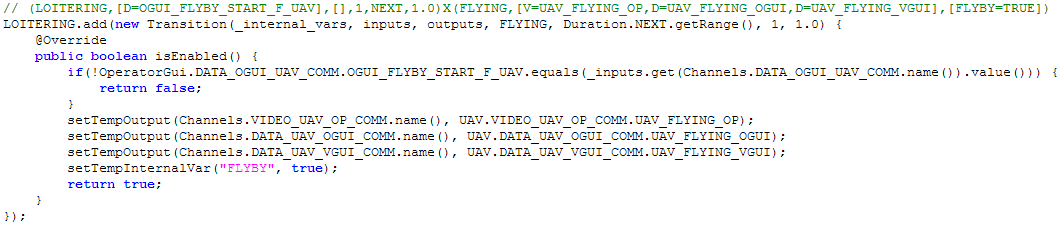
\includegraphics[width=\textwidth]{java_transition.png}
	\label{subfig:subtop}
}
\subfigure[XML Transition]{
	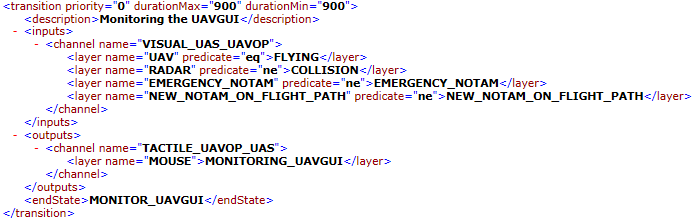
\includegraphics[width=\textwidth]{xml_transition.png}
	\label{subfig:subbot}
}
\caption{Transition Readability Comparison}
\label{fig:read_transition}
\end{center}
\end{figure}

By contrast the Enhanced Operator Function Model (EOFM), an XML based modeling language, can be visualized as a tree-like graph due to the way it is structured~\cite{bass2011toward}.  This visualization allows the modeler to see the hierarchical ordering of actions belonging to a task.  Unfortunately the use of XML to format the model did not provide a similar visualization within the Model Abstraction Framework.  In future work it may be valuable to examine a different XML structure that does allow improved visualization of the model.

\subsection{Modeling Approach and Common Errors}

In chapter~\ref{ch:xmlparser} we addressed some of the challenges of modeling within the Model Abstraction Framework.  In an effort to further reduce the time to model we developed the following modeling approach.  We first defined each Actor in the system and gave them a starting state.  From here we broke the work into task sequences.  Each task sequence represents the path or flow of data through the system, initiating from an external event.  For example our model begins with a \textit{start mission} event that is received by the UAV Operator.  We then implement transitions in sequence until no new transitions are needed.  Each time a new transition is added to the model we run the model to check that the XML is correct and to verify that the new transition is reached.  The full model can be obtained online.  See appendix~\ref{code}.

While this approach was effective it was not a trivial task.  By design the transition sequence moves between Actors requiring the modeler to constantly jump around in the model XML.  Transition sequences will often fork when the action of one Actor causes multiple Actors to respond.  This often results in truncated branches within the model that get forgotten.  In future work it may be necessary to use JPF during the model design so that all paths get checked at each iteration instead of a single path.  

One reason for running the model after adding a new transition is that when the complexity causes modeling errors they typically appear in two fashions.  The first is when an Actor becomes trapped in the current state.  This is the more desirable behavior as it is easier to track down.  The second typical error is an infinite loop.  These can be much more difficult to track down.  Infinite loops are often caused by missing transitions, which are normal during model construction.  If the loop is not caused by a missing transition then more in-depth analysis is needed to find the error.  

While there are many ways to get into an infinite loop we will only mention two common examples.  They are improper transition overriding and uncleared output channels.  Transition overriding happens when you have one transition that is overridden by another before it can fire.  While transition overriding is a desirable behavior, it simulates an interruption, gaps in the transition logic can cause an Actor to continuously cycle between transitions without ever firing a transition and moving to the next state. This can be thought of as undefined behavior.  To fix this, define the behavior for each possible scenario by creating transitions for all combinations of inputs that the Actor cares about.  The simulator will prevent a transition from replacing itself making it better to error on the side of too many transitions.  

The second common error leading to an infinite loop is uncleared outputs.  Uncleared output channels cause an Actor to believe that new input has been received even though it has not, sending the Actor into an infinite cycle.  It is often best practice to clear an Actors outputs once those outputs are no longer being sent across the channel.  This will prevent the target from reading invalid outputs.  If the output values represent a continuous communication that should not be cleared, such as displaying live state information on a GUI, then another approach is to use Actor memory to track changes in input.

While the use of XML to create the model was much more efficient we still feel that a more effective approach to modeling is needed to help standardize the modeling format and prevent common errors.  Whether this approach is a different XML structure, an entirely new format, or a GUI interface that helps visualize the data flow and transition sequences we leave to future work.
\end{comment}

\section{Model Results}

We created three scenarios by adding small variations to the model.  The first scenario involved an uneventful flight.  The second scenario involves the UAV Operator manually avoiding an emergency NOTAM.  The third scenario involves the UAV automatically avoiding an emergency NOTAM.  The second and third scenarios also involve a possible UAV collision and the ATC adding a NOTAM onto the UAV flight path.  Additionally we added a high workload scenario that involves the UAV Operator being interrupted by another person while deconflicting the UAV.  The respective results are shown in figures \ref{fig:uavop_baseline}-\ref{fig:uavop_conflict}.

For each scenario we have four charts depicting the UAV Operator workload and four charts depicting the ATC workload; we currently ignore the workload for non-human Actors.  The first three charts represent the resource input, resource output, and decision workload.  The last chart shows the combined total workload next to the adapted Wickens' model.  For each chart the y axis represents the workload value while the x axis represents Actor state for the given delta time.  What this means is that the x axis cannot be seen as a normal timeline since each time step represents an arbitrary amount of time.  Instead this should be viewed as a progressive change in Actor workload for each time step where a transition was fired.

The results we obtained from the Model Abstraction Framework are very encouraging due to the general consistency with the expected workload.  Despite a few unexplained anomalies, example in figure \ref{fig:atc_manual}, and some unusual workload spikes, shown in figure \ref{fig:uavop_auto}, we can see that generally the Actors have more workload when performing active tasks and less workload for simple tasks.  A clear example of this is the UAV Operator workload in figure \ref{fig:uavop_baseline}.  The workload spikes while creating the flight plan then remains low while monitoring the UAV GUI for information.  When that information is received we see a small spike followed by a prolonged workload spike while the UAV Operator is deconflicting the flight plan.

\subsection{Inter Actor Comparison}

When comparing the UAV Operator and ATC baseline workload, shown in Figures \ref{fig:uavop_baseline} and \ref{fig:atc_baseline}, the relationship between the UAV Operator and the ATC becomes very clear.  For this scenario the UAV Operator creates a flight plan for the mission.  When the UAV Operator finishes the flight plan it is sent to the FAA Server where it is flagged to be approved by the ATC.  The ATC then performs the approval and returns back to normal operations.  The UAV Operator receives the approval and begins normal mission operations that increase the workload.  This is reflected beautifully in the Actor workload.  The UAV Operator workload spikes during flight plan creation then flat lines while waiting for a response.  Once the UAV Operator receives the response their workload spikes again as they perform the mission.  The ATC workload is just the opposite, spiking while approving the flight plan and returning to normal afterwards.  The comparison of the other scenarios show the same correlations.  

\begin{figure}[p]
\begin{center}
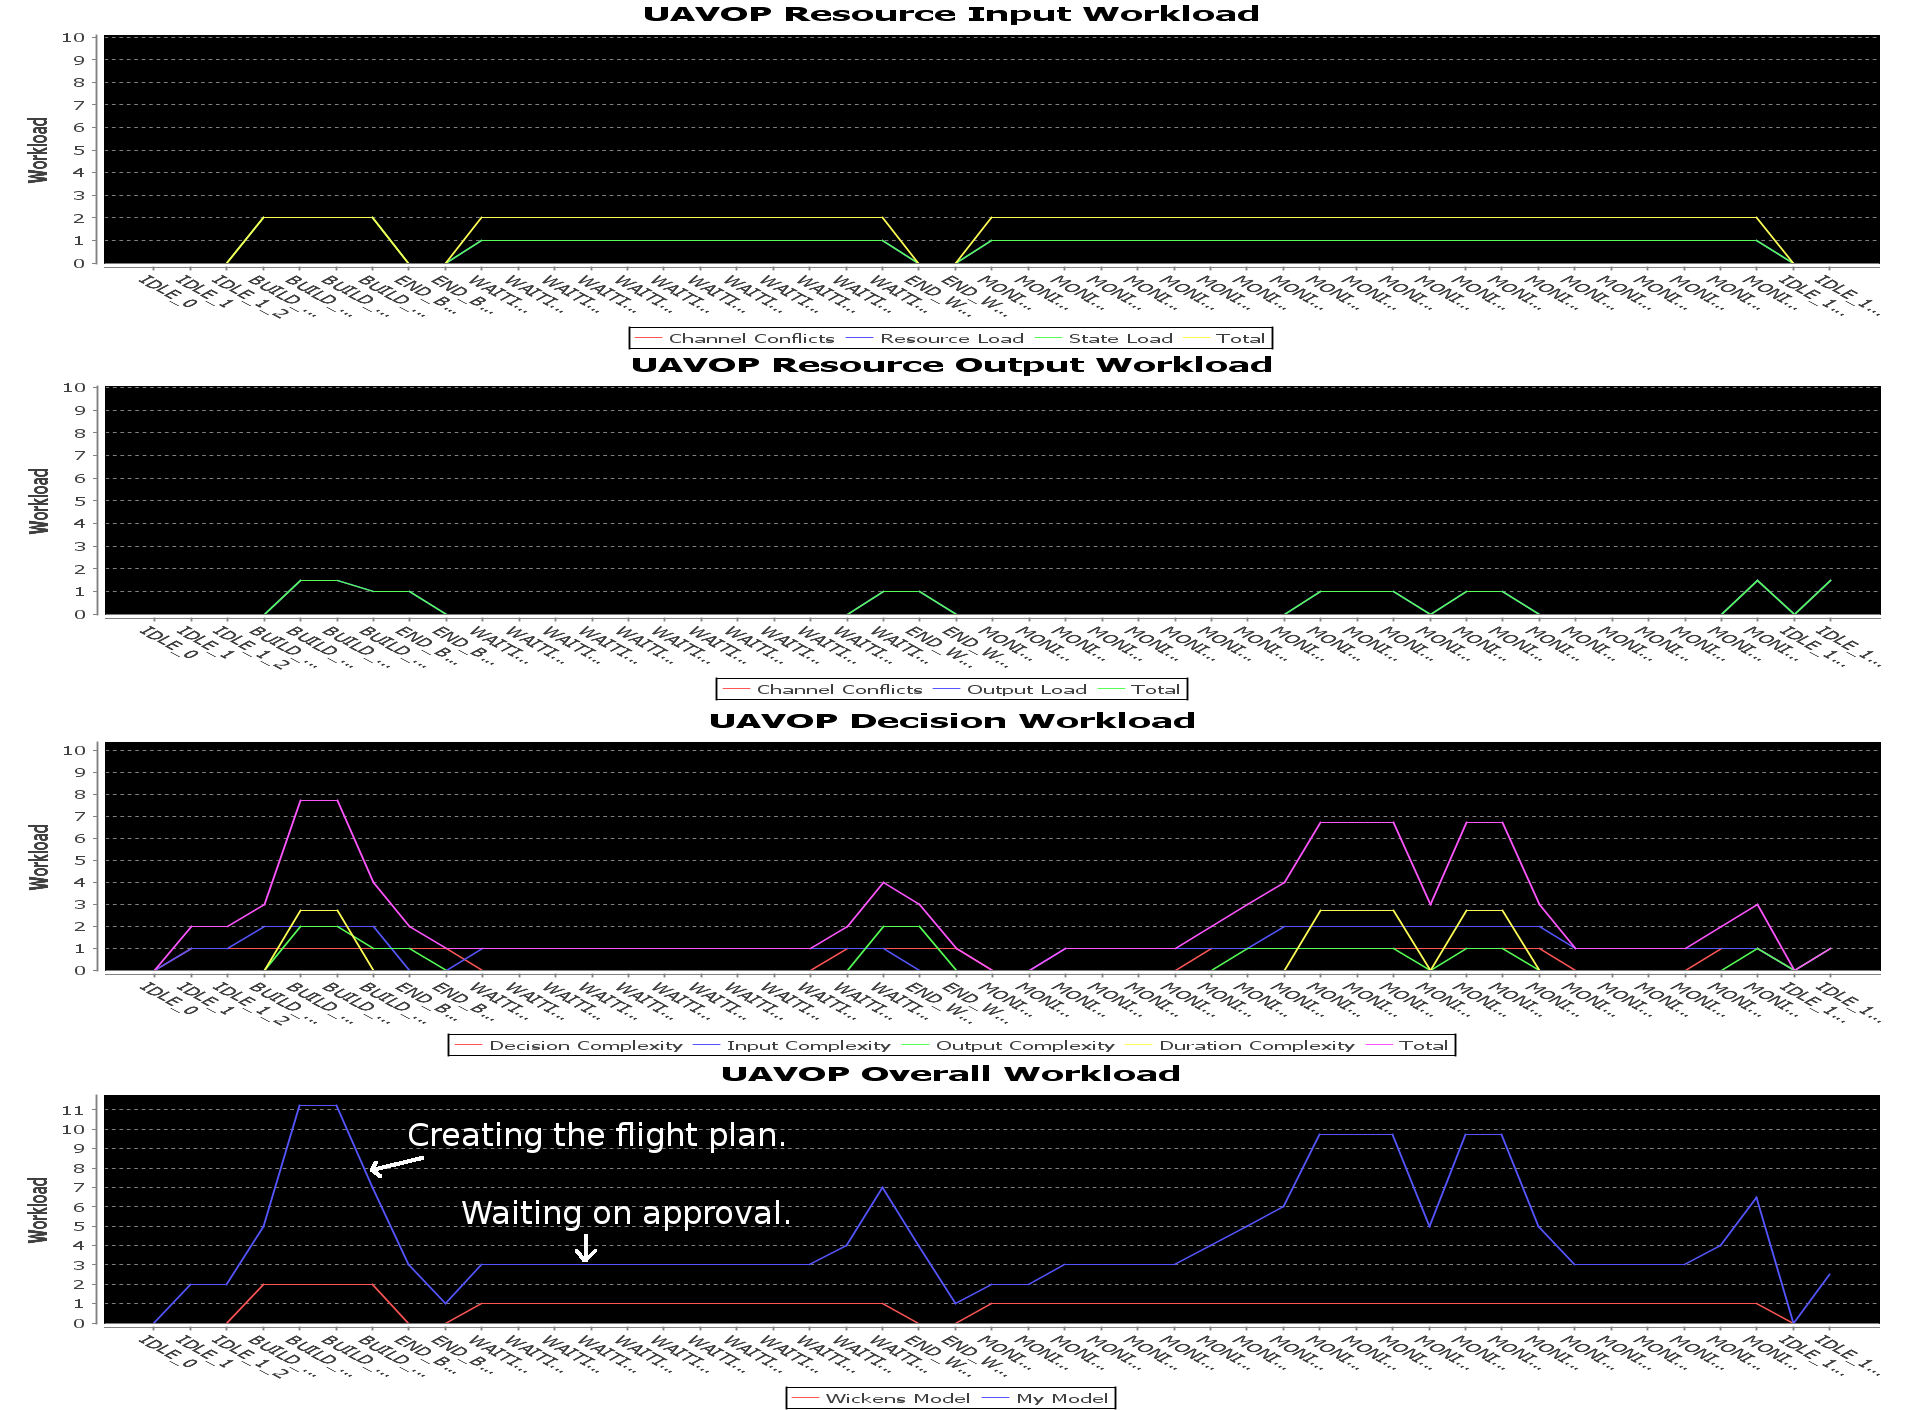
\includegraphics[width=\textwidth,height=\textheight]{UAS_in_NAS_no_events_UAVOP.png}
\vspace{-25pt}
\caption{UAV Operator: Baseline}
\label{fig:uavop_baseline}
\end{center}
\end{figure}

\begin{figure}[p]
\begin{center}
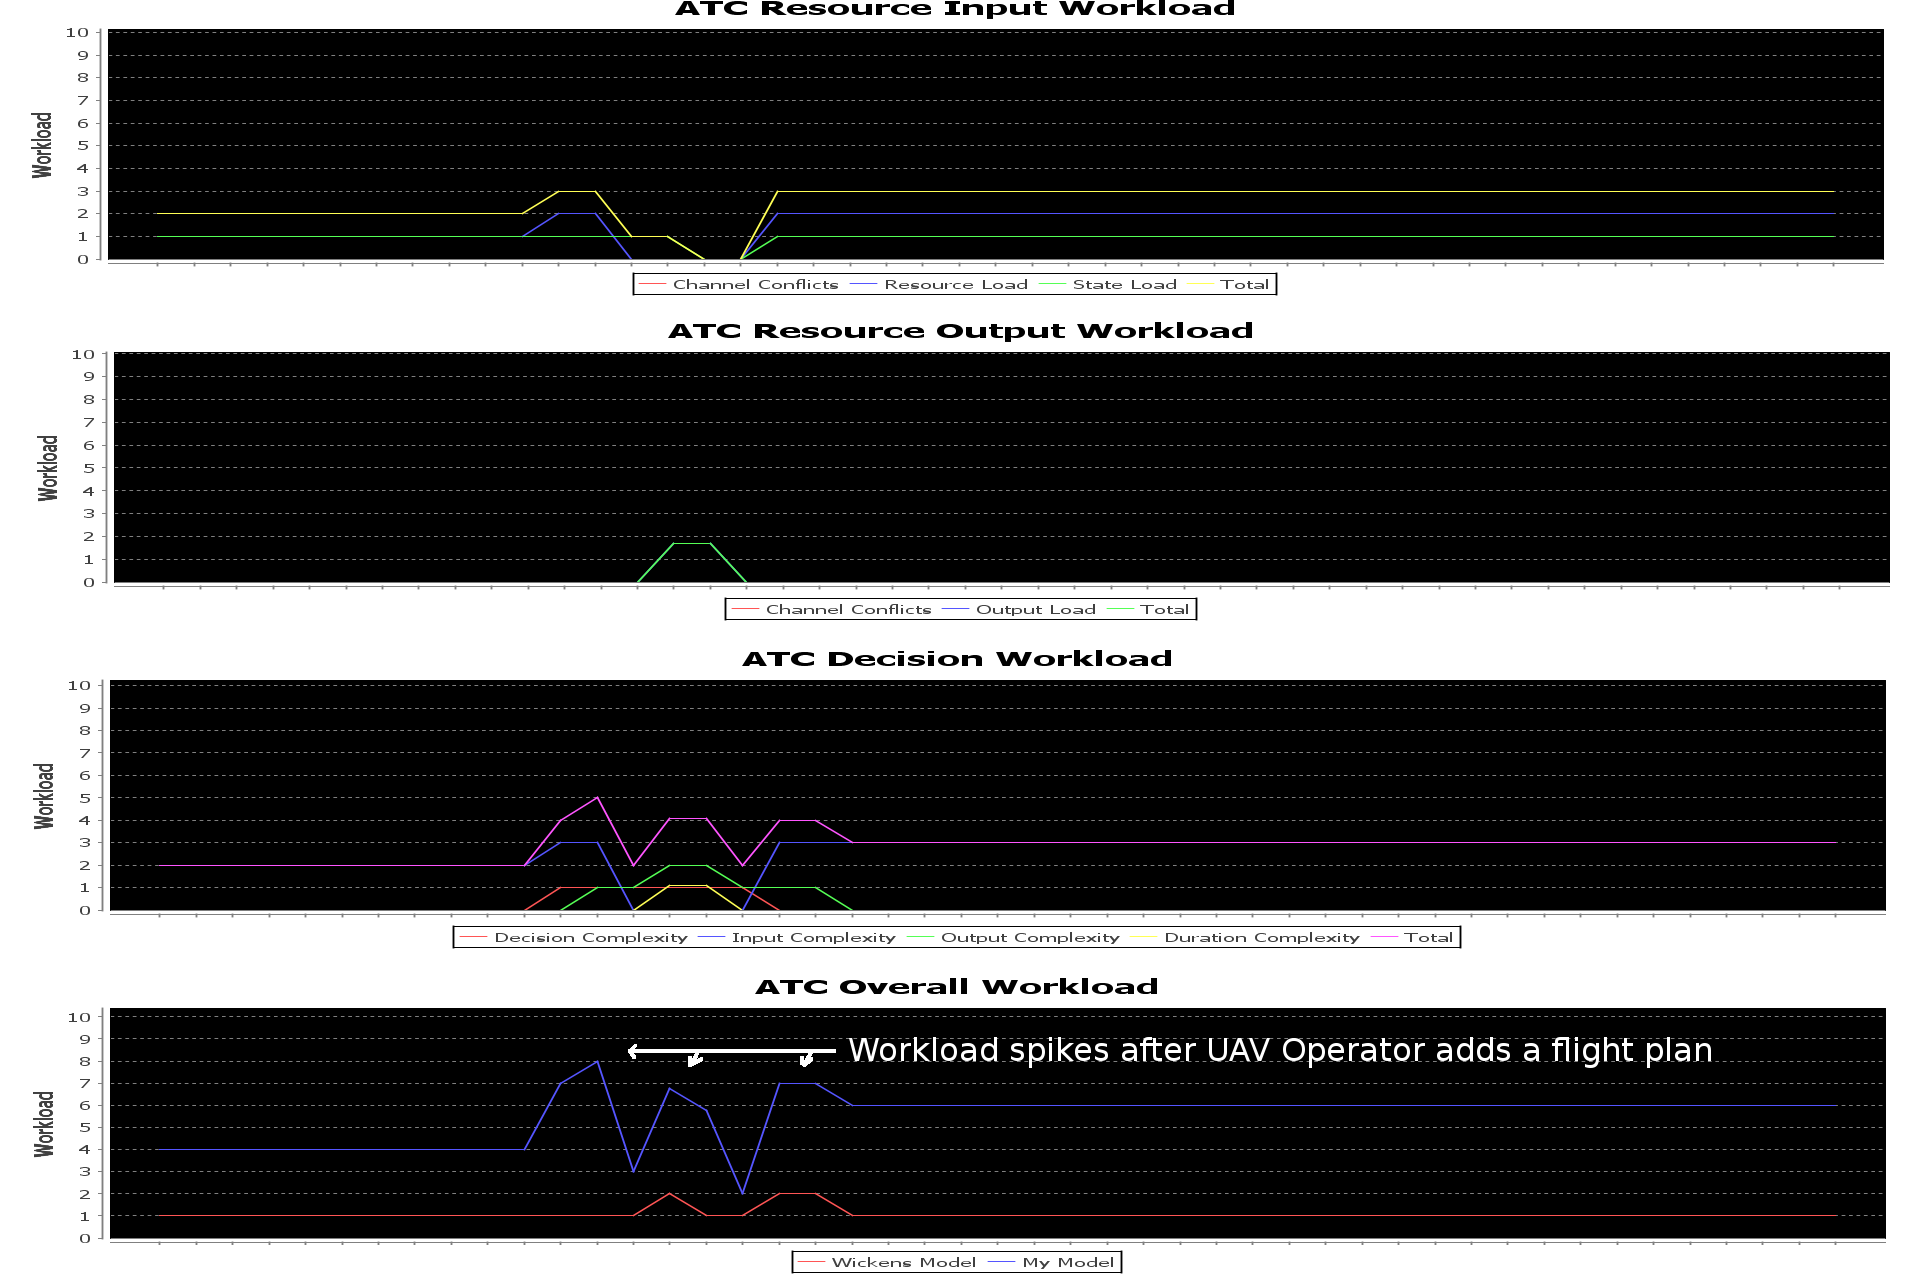
\includegraphics[width=\textwidth,height=\textheight]{UAS_in_NAS_no_events_ATC.png}
\vspace{-25pt}
\caption{ATC: Baseline}
\label{fig:atc_baseline}
\end{center}
\end{figure}

We also see the effects of the UAV Operator and ATC relationship in the \textit{manual avoid} scenario, shown in Figures~\ref{fig:uavop_manual} and \ref{fig:atc_manual}, when the delayed action of the UAV Operator causes the ATC to remain in the \textit{avoid conflict} state for an abnormally long period of time.  By looking at the Actor state we see that the UAV Operator was already in the process of deconflicting the UAV and was not able to immediately respond to the ATC emergency NOTAM.  The \textit{auto avoid} scenario, shown in Figures~\ref{fig:uavop_auto} and \ref{fig:atc_auto}, shows an improvement in this regard as the UAV automatically avoids the emergency NOTAM while the UAV Operator is busy.  This example demonstrates how the workload modeling allows us to detect problems using the model and then analyze fixes to those problems.

\begin{figure}[p]
\begin{center}
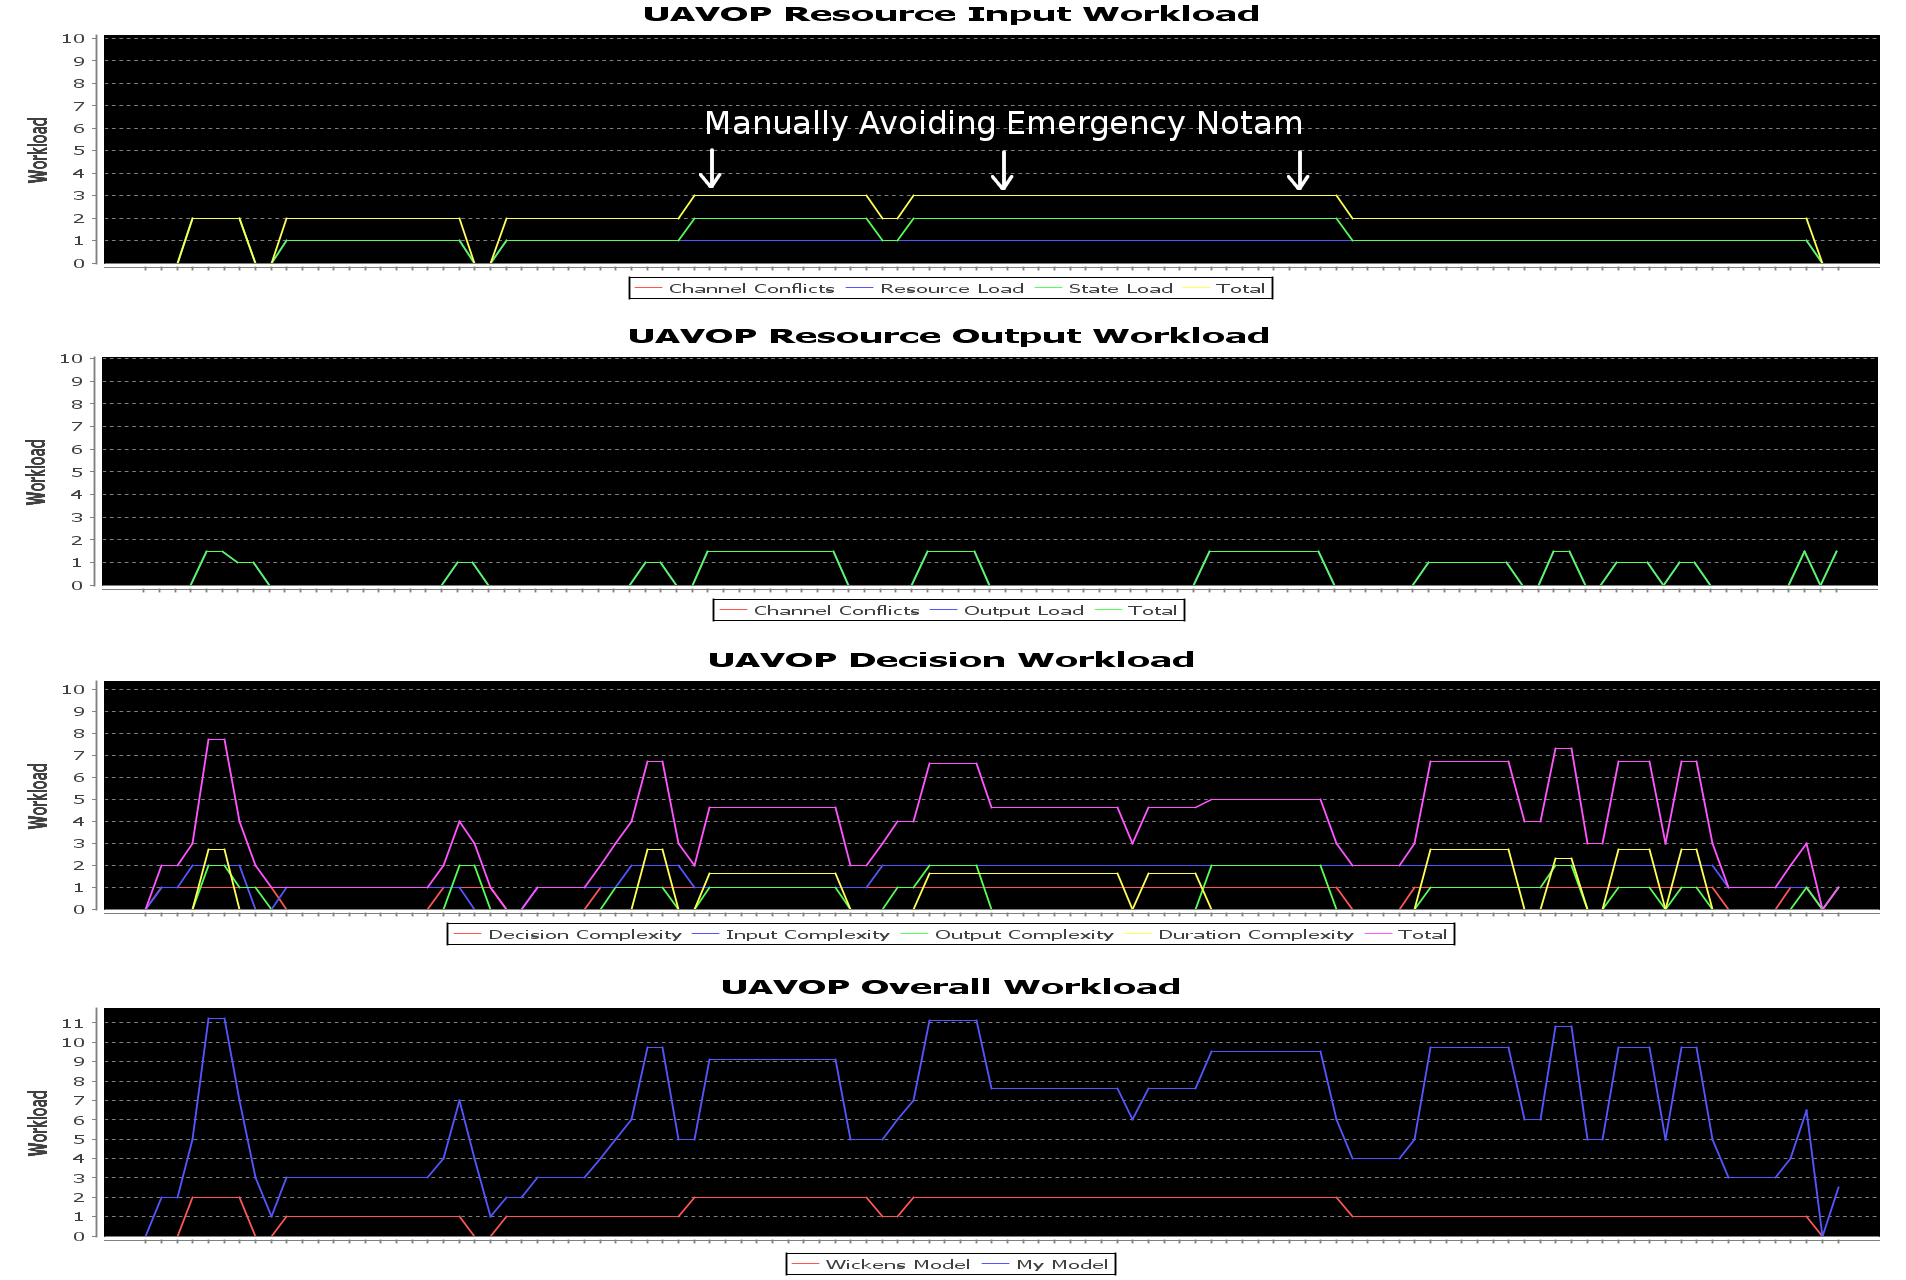
\includegraphics[width=\textwidth,height=\textheight]{UAS_in_NAS_manual_emergency_notam_UAVOP.png}
\vspace{-25pt}
\caption{UAV Operator: Manually Avoided Emergency NOTAM}
\label{fig:uavop_manual}
\end{center}
\end{figure}

\begin{figure}[p]
\begin{center}
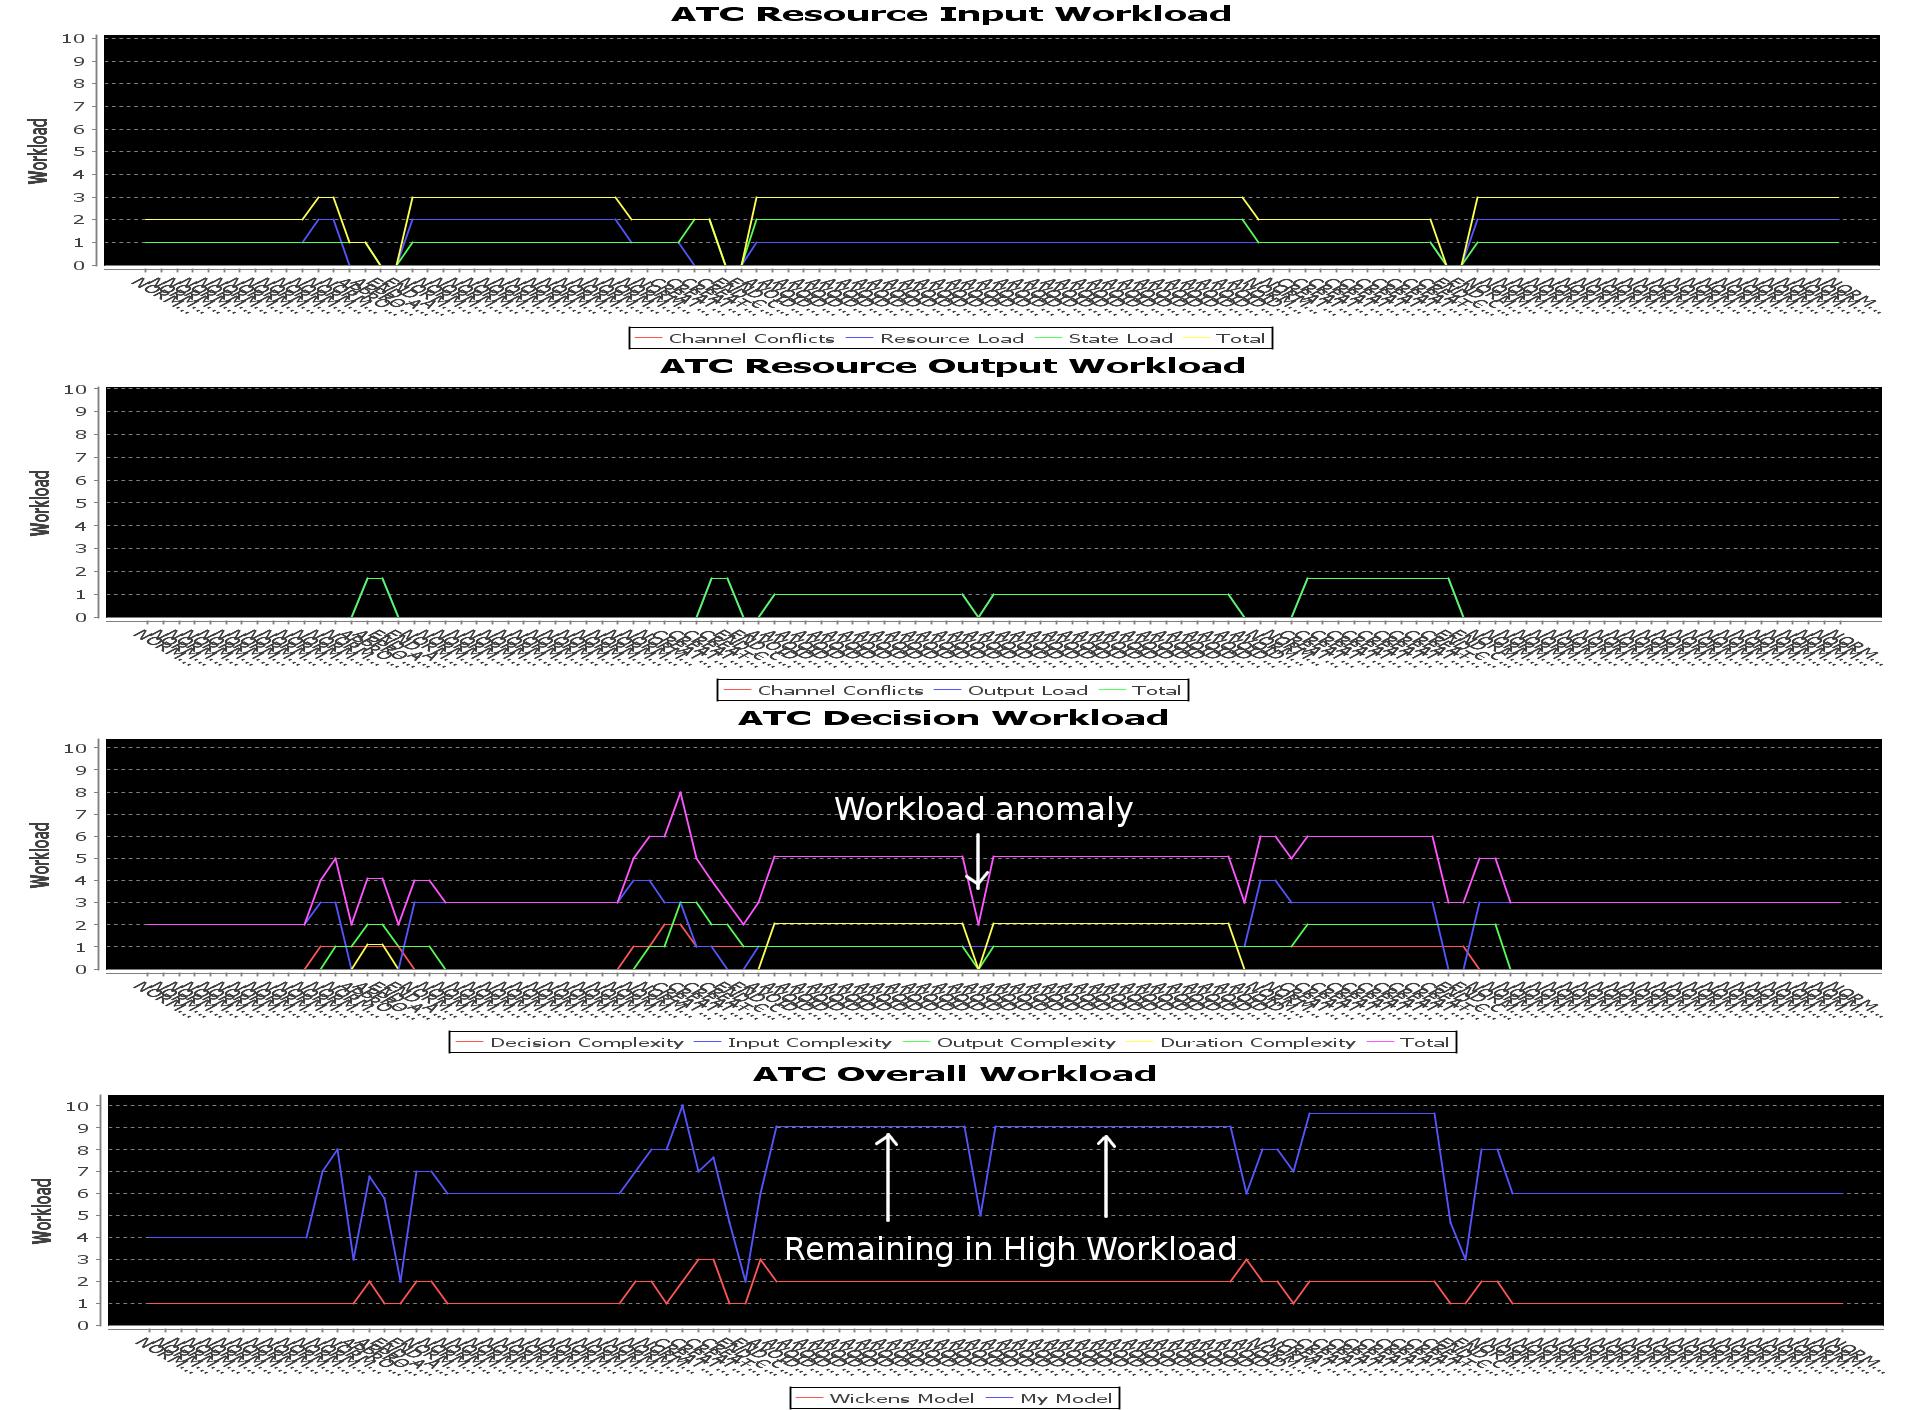
\includegraphics[width=\textwidth,height=\textheight]{UAS_in_NAS_manual_emergency_notam_ATC.png}
\vspace{-25pt}
\caption{ATC: Manually Avoided Emergency NOTAM}
\label{fig:atc_manual}
\end{center}
\end{figure}

\subsection{Intra Actor Comparison}

At first glance the UAV Operator workload between the \textit{manual avoid} scenario, Figure~\ref{fig:uavop_manual}, and the \textit{auto avoid} scenario, Figure~\ref{fig:uavop_auto}, appear almost identical.  This is good as these scenarios are nearly identical.  Upon closer examination we see that when the UAV Operator has to manually avoid the emergency NOTAM there is a prolonged increase in resource input workload, an extra spike of resource output workload, and a noticeable spike in decision workload once the UAV Operator begins the process of avoiding the NOTAM.  This results in a significant workload spike compared to the more stable workload seen in the \textit{auto avoid} scenario.  Another less noticeable difference is that the manual emergency NOTAM avoidance takes longer to complete than the auto avoid feature, something that is critical in these types of situations.

\begin{figure}[p]
\begin{center}
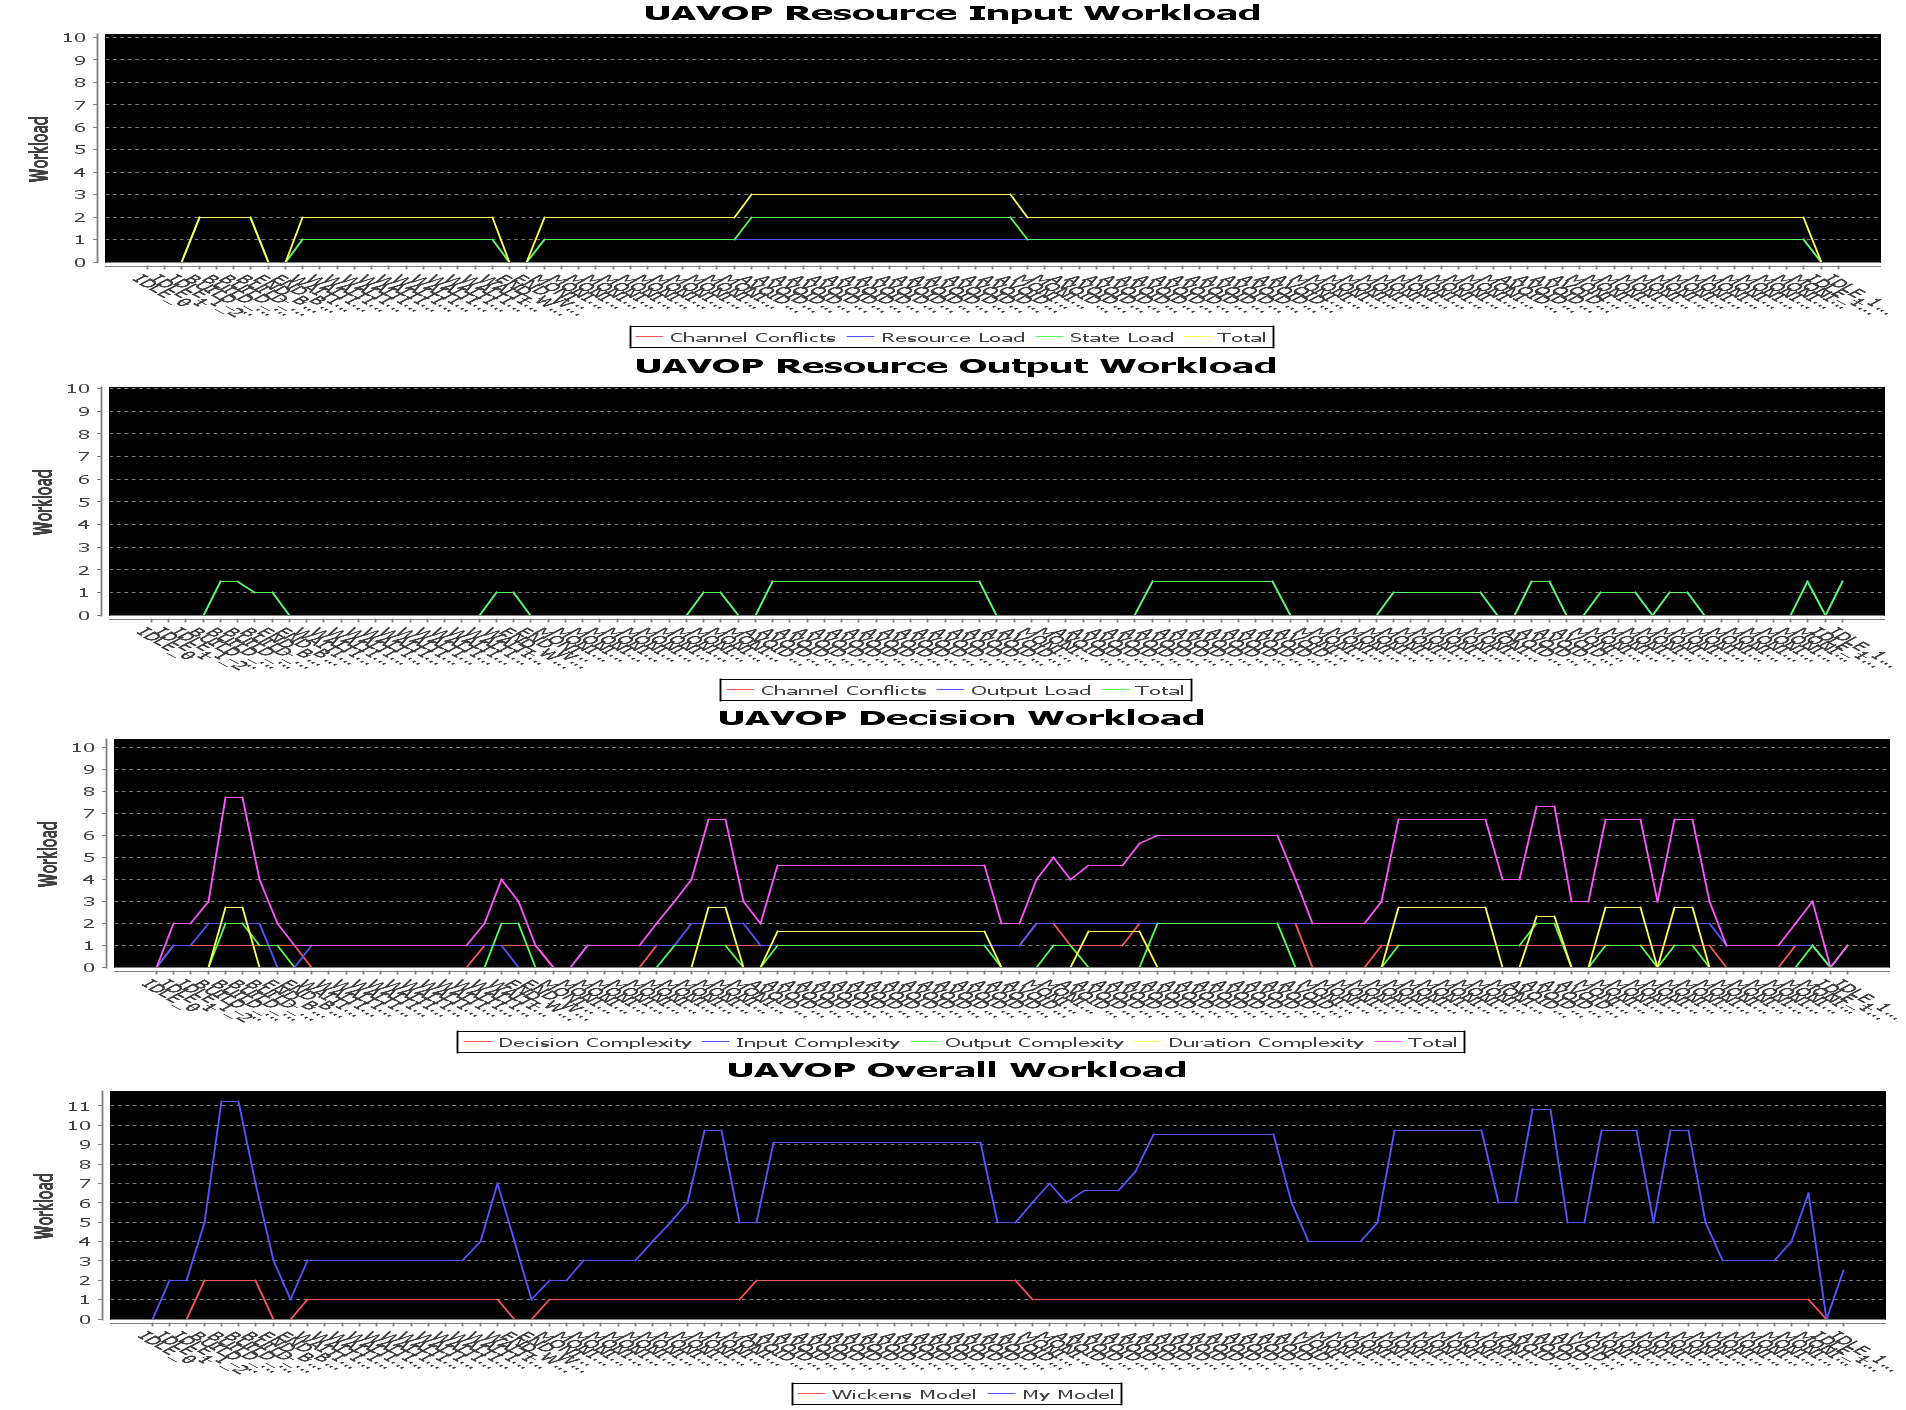
\includegraphics[width=\textwidth,height=\textheight]{UAS_in_NAS_auto_emergency_notam_UAVOP.png}
\vspace{-25pt}
\caption{UAV Operator: Auto Avoid Emergency NOTAM}
\label{fig:uavop_auto}
\end{center}
\end{figure}

\begin{figure}[p]
\begin{center}
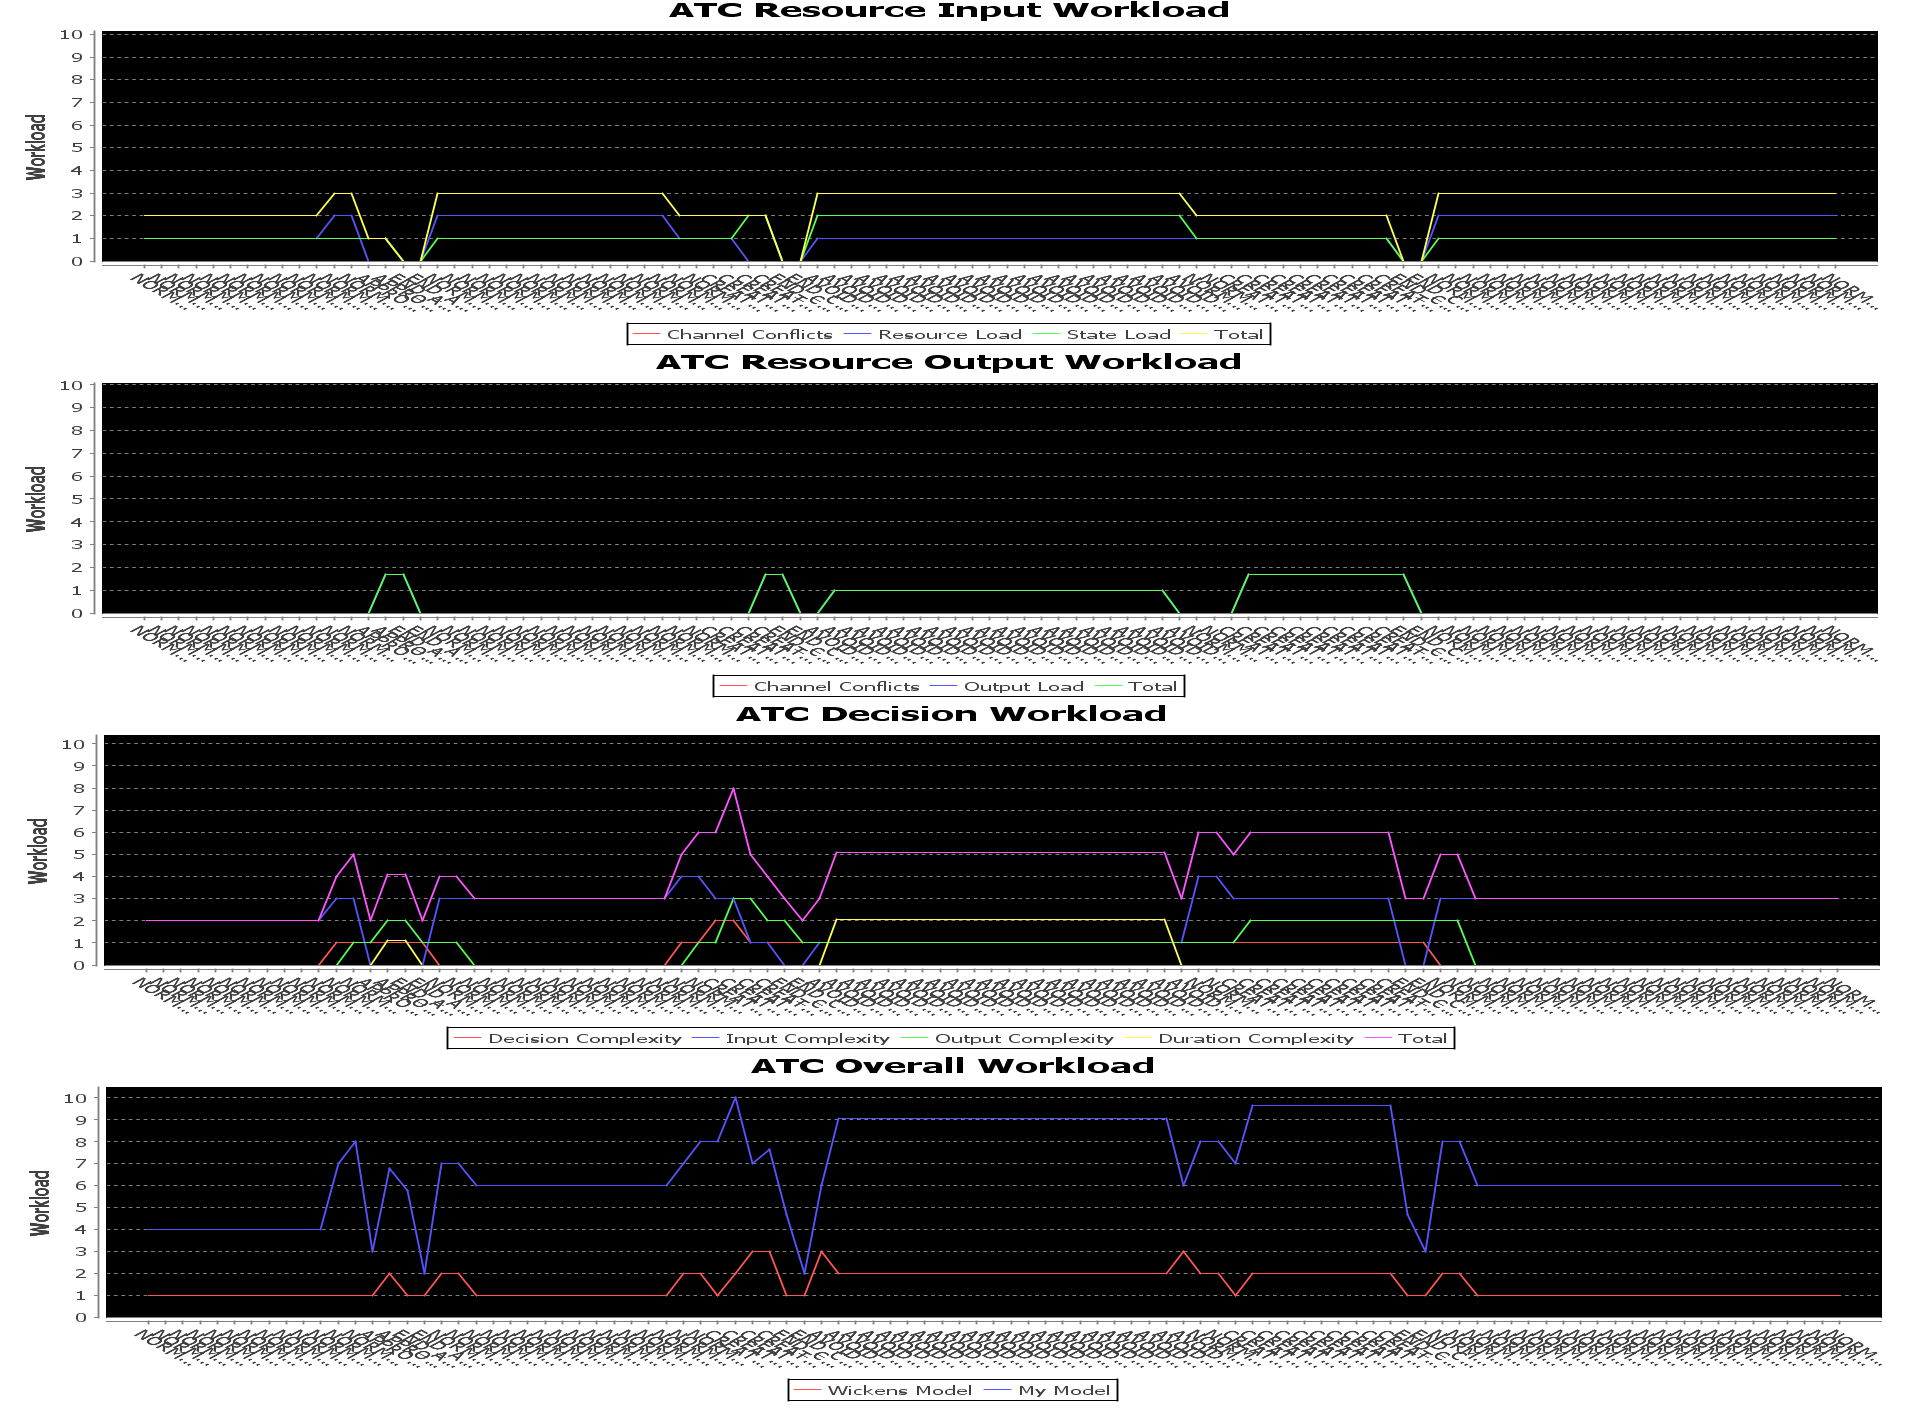
\includegraphics[width=\textwidth,height=\textheight]{UAS_in_NAS_auto_emergency_notam_ATC.png}
\vspace{-25pt}
\caption{ATC: Auto Avoid Emergency NOTAM}
\label{fig:atc_auto}
\end{center}
\end{figure}

To make this simple model a little more interesting we decided to add an interruption to the \textit{auto avoid} scenario.  See Figure \ref{fig:uavop_conflict}.  When the UAV Operator begins the first deconfliction procedure he or she is interrupted by another person, a dummy Actor added to the model just for this interruption.  Instead of ignoring this interruption the UAV Operator attempts to communicate with this person while still performing the deconfliction procedure.  This results in a visual channel conflict as the UAV Operator is watching both the UAS GUI and the person that caused the interruption.  In addition to this the UAV Operator is now in a high load/multi tasking state.  The result is a workload value of 20, almost double the next highest workload value seen in the simulation.

\begin{figure}[p]
\begin{center}
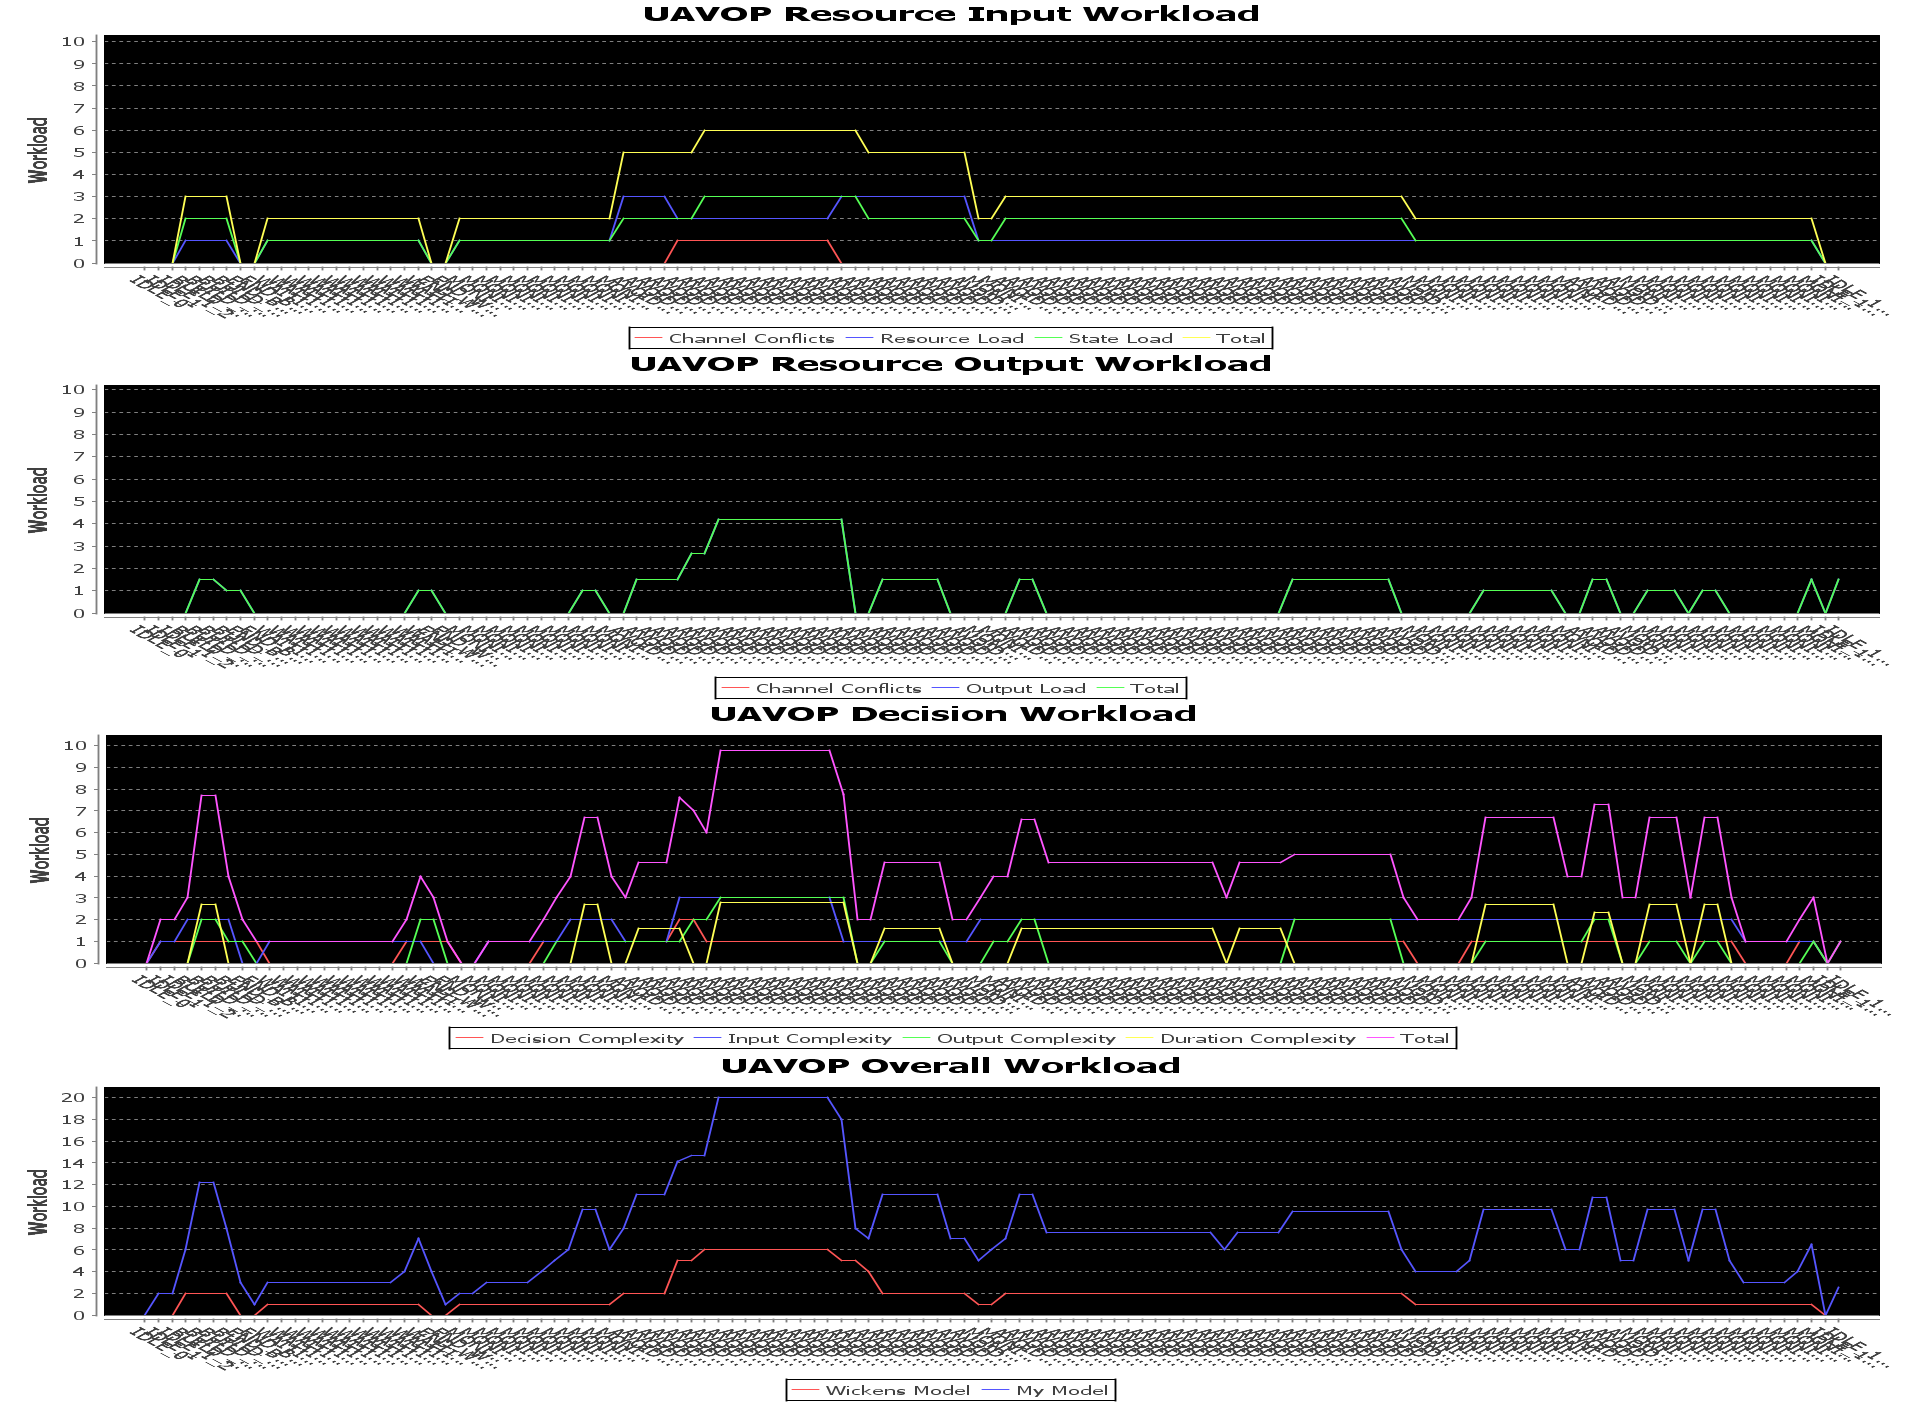
\includegraphics[width=\textwidth,height=\textheight]{UAS_in_NAS_channel_conflict_UAVOP.png}
\vspace{-25pt}
\caption{UAVOP: Auto Avoid Emergency NOTAM w/ Interruption}
\label{fig:uavop_conflict}
\end{center}
\end{figure}

While we are mostly pleased with the workload results there are a few anomalies in the results that are misleading.  The most commonly occurring anomaly is a drastic decrease in workload followed immediately be an equally drastic increase in workload, see figure~\ref{fig:atc_manual}.  This tends to happen when an Actor is transitioning into the same state it just left.  The spike happens because we are collecting metrics twice for each step in the delta clock; once right before the active transitions are fired and once after they are fired.  In future work we may collect specific metrics once per delta clock step to prevent these anomalies.

\subsection{Workload Analysis}

To view the metric data more clearly we split the data into four different charts that represent the \textit{resource input workload}, \textit{resource output workload}, \textit{decision workload}, and \textit{overall workload}.  In the \textit{resource input workload} chart we get an idea of how many channels, layers, and memory objects the Actor is observing.  By comparing this with the \textit{resource output workload} we can see when the inputs occasioned a response from the Actor.  For the most part these charts are well behaved and follow the workload patterns that we know about.

On the other hand the \textit{decision workload} typically jumps all over the place.  While we believe the increase in \textit{decision workload} does in fact increase \textit{overall workload}, we are unsure how to weight this value in comparison with the \textit{resource workload}.  This is something that needs to be verified through sensitivity and user studies in future work.

The last analysis we would like to make is the comparison of our workload metric to that of the adapted Wickens' model from chapter~\ref{ch:workload}.  The general flow of the two metrics is very similar, as is expected since everything in the Wickens' model also exists in our workload metric.  What is more interesting is where the two metrics differ.  Our workload metric is comprised of 9 different values each of which can range from zero to two or more.  This adds a fair amount of detail into the workload measurement.  An example of this can be seen in the \textit{auto avoid} scenario shown in Figure~\ref{fig:uavop_auto}.  After avoiding the emergency NOTAM the UAV Operator continues to monitor the UAS GUI eventually avoiding another potential conflict.  The adapted Wickens' model shows a flat line during this portion of the scenario while our metric shows a heart beat that correlates with the UAV Operator actions.  


\chapter{Summary and Future Work} \label{ch:summary}

As part of this thesis work we have developed the Model Abstraction Framework.  This simple modeling framework allowed us to experiment with generating different types of raw data from a human-machine model.  The modeling framework uses the concepts of Directed Role Graphs and Directed Team Graphs to build models constrained by specific behavior and communication.  The framework then takes this model and converts it into a labeled state transition system that is run on the simulator.  During the simulation we collect raw data from the states, transitions, and labels.

Using this raw data we have demonstrated the generation of three workload metrics: Adapted Wickens' Model, Resource Workload Metric, and Decision Workload Metric.  The Adapted Wicken's Model, our baseline metric, is an adaptation of a simple model meant to measure cognitive resource load~\cite{wickens2002multiple}.  The Resource Workload Metric, based off of the cognitive workload category presented by Jared et al. \cite{moore2014modeling}, represents the cognitive resource load from inter-actor communication and memory access.  The Decision Workload Metric, based off of the algorithmic workload category presented by Jared et al. \cite{moore2014modeling}, represents the complexity of the decision making process.

Using these metrics we demonstrated two important results.  The first result is a general consistency between our baseline model, Adapted Wickens' Model, and the combination of the Resource and Decision workload metrics.  While the Resource and Decision workload metrics are more expressive they trend very closely with the Adapted Wickens' Model.

The second result was a general consistency with the known high and low workload periods observed during the UAV Enabled Wilderness Search and Rescue (WiSAR) flight tests.  Indeed the results from the Resource and Decision workload metrics was more closely aligned to our observations than that of the Adapted Wickens' Model.

Additionally we are encouraged by the predicted workload reduction observed when we introduced automation into scenario three of the case study.  The ability to predict workload reduction with models is one of the primary objectives towards reducing the number of human required to operate a UAS.

\section{Threats to Validity}

While these results are encouraging we realize that they do not yet represent human workload.  The Model Abstraction Framework was developed to enable experimentation with the generation of raw data.  No studies have been performed showing that the Model Abstraction Framework can accurately model human-machine systems.  No work has been done to show that the raw data generated by the framework correlates to memory usage, decision making, cognitive resource usage, and other recognized aspects of human workload.

The baseline workload results were generated by the Model Abstraction Framework and not by a separate modeling framework that has been shown to correctly model human-machine systems and cognitive resource load.  Since there is no guarantee that converting the model used by the Model Abstraction Framework to another modeling language produces the same model we chose to instead attempt to convert the workload metric from a task based paradigm to a state/transition based paradigm.

The WiSAR high and low workload profile used for validating workload consistency is not the result of actively measuring different aspects of human workload during a flight test.  Instead the workload profile was obtained from in-flight observations and post-flight surveys for a limited number of flight tests.

\begin{comment}
We have shown that the Model Abstraction Framework is extremely flexible, allowing each portion of a system to be modeled at varying levels of abstraction.  This allows us to model system components without knowing the implementation details.  We demonstrated this in the UAV Enabled Wilderness Search and Rescue (WiSAR) case study when we found flaws in the Video Operator role that were previously undocumented and again in the Unmanned Aerial System integration into the National Airspace System case study when we demonstrated the effect of automating a portion of the UAV Operator duties.  

Additionally we have demonstrated our ability to perform model checking directly on the Model Abstraction Framework models using Java Pathfinder (JPF).  By creating models directly in Java there is no need for an extra conversion to a model checking platform.  We also have the ability to create multiple paths through the model with the use of transitions, transition duration ranges, and events. While we leave it to future work to fully realize the potential of model checking the Model Abstraction Framework with JPF we believe this forms the basis of an extremely powerful modeling tool.

We demonstrated the ability to implement an XML model parser to facilitate more efficient modeling.  While the improvement the XML provided was not as great as we had hoped this does demonstrate the ability to adapt to more efficient methods of modeling.  One area of future work is to implement conversion classes between our modeling language and some of the other more popular modeling languages such as Brahms or EOFM.  This would give us additional validation options ~\cite{bolton2013litreview}.

Finally we have demonstrated the ability to extract workload metrics that are consistent with known high workload events and closely related to human workload theories such as Multiple Resource Theory, Threaded Cognition Theory, and Operator fan-out~\cite{wickens2002multiple, salvucci2008threaded, cummings2007predicting}.  We are encouraged by the predicted workload reduction seen in our second case study when we used variations in our model to represent the effects of automating a human performed task.  And we will use this idea of predicting workload to reduce actual operator workload as a seque into the future of this work.
\end{comment}

\section{Future Work}

The ultimate goal of this work is to create a UAS for WiSAR that allows a single human to perform all of the necessary tasks.  In order to achieve this goal there is still a lot of work to be done.  This thesis represents the beginning phase of this research, which is to begin comprising workload metrics.  The next phase will be to modify and validate that the metrics reflect human workload, and the last phase will be to show that the predicted workload reductions are indeed reductions in human workload.

This work focuses on two facets of human workload, cognitive resource load and decision complexity.  To predict human workload more facets must be explored.  Jared et al. \cite{moore2014modeling} are expanding on these metrics by experimenting with a temporal workload category\cite{moore2014modeling}.  They are also developing second and third order metrics within all three workload categories.  Additionally it may be necessary to expand the scope of the human workload categories before a moderately accurate measure of human workload can be obtained.

The next step will be to find the correlations between the different workload aspects in order to use the correct ratios to predict workload.  Once a metric profile for measuring human workload has been achieved, there may be many, the next phase of modifying and validating the metrics begins.




\appendix
\chapter{UAS-enabled WiSAR Proposal} \label{app:uas_wisar}

This appendix is a proposal to create a UAS for the UE-WiSAR domain.  This represents the initial step towards our ultimate goal of reducing the number of humans in a UAS.  During the requirement gathering and design phase of the project it became clear that in a system this complex the right design was paramount to success.  Instead of blindly pressing forward with the software development we decided that the more important scientific problem was to figure out how to model and validate the system design before implementation.  

\section{INTRODUCTION}
Advances in Micro Unmanned Aerial Vehicle (mUAV) technology has pushed mUAVs
into new frontiers.  UAV Enabled Wilderness Search and
Rescue (UE-WiSAR), one of these frontiers, has been a focus of the Human
Centered Machine Intelligence (HCMI), Multiple Agent Intelligent Coordination and Control (MAGICC) and Computer Vision (CV) labs at Brigham Young University since 2005.  In that time research has
been conducted on human interaction with mUAVs, improving target detection by
enhancing video taken from a mUAV, integrating mUAVs into a SAR environment,
and improving the mUAVs chance of getting video footage of the target.  Over
the course of this research many of the ideas for improving UE-WiSAR results
have been validated through simple experiments and user studies.  Live Field
Demo's with actual Search and Rescue personnel have also shown favourable
results. These results represent important progress in Human Robot Interaction. 

Although the research has proven successful, many of the tools developed for
UE-WiSAR are unfit to share with a broader community.  This proposal outlines
the challenges faced by UE-WiSAR, the solutions discovered for overcoming these
challenges and a plan for creating UE-WiSAR software that incorporates said
solutions into a stable software package as part of an industrial thesis.  As an
industrial thesis the emphasis is not on new research but on delivering high
quality software

\section{PREVIOUS WORK}
One goal of this project is to take past research and present it in a software
application that encourages future researchers to use the software as a
framework for continued research.  Essentially what this means is that the
entire purpose of developing the UE-WiSAR software is to make it available
to future researchers and, more importantly, practicing searchers.  The majority
of the referenced work comes from a combined effort from the HCMI, MAGICC, and CV labs at BYU and focuses on solving
the specific problems that arise when bringing a small UAV into the WiSAR arena.
This proposal represents the realization of this goal
\cite{lin2010supporting}.
  
  
\section{WiSAR}
\subsection{The Problem}
Wilderness Search and Rescue (WiSAR) is more prevalent today then in any other
time in history.  While Search and Rescue has been around since the beginning of
mankind \cite[p.~13]{setnicka1980}, the improved communications and increased
accessibility to wilderness areas have caused an increase need for WiSAR
operations.  Often times these operations have limited resources due to limited
funds, remote locations, and dangerous conditions.

% Furthermore, the paradigm shift that government agencies,
% instead of the individual, are responsible for personal
% safety \cite[p.~viii]{setnicka1980} has created a strain on local government
% agencies to provide effective SAR operations.  To add to this pressure a
% prolonged WiSAR operation can be exorbitantly expensive ``citation''.  This
% increasing pressure has prompted research to provide more effective SAR tools
% while lowering SAR costs.

\subsection{Concepts}
% Search and Rescue implies searching for an individual and then rescuing them
% once found.  With UAV's this is slightly different.  These UAV's will probably
% never be capable of performing the actual rescue.  This means that while
% classified as Search and Rescue the role performed by the UAV is strictly a
% searching role.  This means that UE-WiSAR is not necessarily useful for all
% WiSAR operations.  

To help understand how UE-WiSAR will be effective, some WiSAR
concepts, defined by T.J. Setnicka \cite[p.~35]{setnicka1980}, will be used. 
The first concept is the four core elements of a WiSAR operation.
\begin{figure}[h]
	\begin{center}
		\begin{math}
			Locate \Rightarrow Reach \Rightarrow Stabilize \Rightarrow Evacuate
		\end{math}
	\end{center}
	\caption{Core SAR Elements}
\end{figure}

The second concept is the WiSAR plan and its components, specifically Strategy
and Tactics.  Strategy is the process of gathering information and making an
accurate assessment of the situation.  Tactics are outlined solutions for
specific situations that can be used as part of a Strategy.


% This basic understanding of WiSAR core elements and
% plan components are important to understand the definitions referred to
% throughout this proposal.  These concepts represent how UE-Wisar software will
% be effective in traditional WiSAR operations.

\subsection{Searching}
% In each WiSAR operation the time spent in each of the core elements is
% different.  Some operations may spend the majority of time in reaching and
% evacuating the person.  No other SAR elements can be accomplished, however,
% until the person is located.  This typically represents the majority of time
% spent if the person is missing.  Locating an individual in the wilderness can be
% a daunting task.  SAR commanders develop Strategies for locating the person and
% use the Tactics available to them as part of those Strategies.  Each Tactic
% applied to a search is based on availability, effectiveness, and cost.  One
% Tactic that has proven it's effectiveness is aerial surveillance.  One large
% drawback to this Tactic is the cost.  Until recently most aerial surveillance
% has been done with piloted aircraft.  Advances in Unmanned Aerial Vehicles (UAV)
% have created new options for providing aerial surveillance, however, high-end
% commercial UAV's are still incredibly expensive.  This has prompted a deeper
% look into mUAV which are low-cost but by their very nature have a long list of
% obstacles that need to be overcome before they can be effective.
Locating an individual in the wilderness can be a daunting task and typically
represents the majority of time spent on an operation if the person is missing.
SAR commanders develop Strategies for locating the person and use the Tactics
available to them as part of those Strategies.  Each Tactic applied to a search
is based on availability, effectiveness, and cost.  One Tactic that has proven
it's effectiveness is aerial surveillance.  One large drawback to this Tactic is
the cost and availability.  Until recently most aerial surveillance has been
done with piloted aircraft.  Advances in Unmanned Aerial Vehicles (UAV) have
created new options for providing aerial surveillance, but high-end
commercial UAVs are still incredibly expensive.  This has prompted a deeper
look into using mUAVs that are low-cost but by their very nature have a long
list of obstacles that need to be overcome before they can be effective.

% \section{THESIS}
% Overcoming the obstacles of using mUAV for WiSAR operations has been a primary
% research focus at BYU since 2005.  In that time many solutions have been found
% to overcome these obstacles.  These solutions will be outlined in greater detail
% later in the proposal.  In the process of discovering these solutions a lot of
% software was created.  This software was then used in user tests to determine
% it's effectiveness.  Also, many studies where conducted in understanding SAR,
% human mUAV interaction, and mUAV-WiSAR integration.  These software pieces along
% with the knowledge of how to use them for WiSAR is incredibly valuable. 
% Unfortunately the software that has been created is disjointed and unstable. 
% Much of the software was written as prototypes for user studies and is not fit
% for distribution individually or as a whole.  \textbf{The UE-WiSAR proposal is
% to combine these prototypes into a cohesive and stable software package,
% designed as a new Tactic, for distribution to the SAR, mUAV, and research communities.}
% 
% ``The value of an idea lies in the using of it.'' -Thomas A. Edison

\section{WHY DEVELOP UE-WiSAR}
\subsection{New Search Tactic}
As mentioned earlier, most WiSAR operations are limited in the search Tactics
they can use.  Using mUAVs offers a new aerial surveillance Tactic.  The mUAVs
are small and relatively inexpensive; cost estimates are between \$1,000 and
\$10,000 per mUAV
\cite{goodrich2008supporting,goodrich2007using,adams2007camera}.
These platforms represent a small fraction of the possible mUAVs that are capable of performing
UE-WiSAR tasks.  One model that is currently receiving attention is the
multi-rotor mUAVs which can move at slow speeds and remain stationary if needed
\cite{almurib2011control}.  The relatively low cost of these mUAVs makes them
attractive for aerial surveillance.  mUAVs also reduce the risk to search
personnel in the event of critical user/equipment failure.  Also, future work
will allow for multiple simultaneous mUAV surveillance 
\cite{waharte2009coordinated}.  

While very capable, mUAVs are not fit for every
situation.  Few battery-powered mUAVs can stay aloft with the required
camera-equipment for more than 90 min, many for less than half that time.  This means that mUAVs are
limited in their search range and effective search time. Also, the mUAV is
extremely suseptible to high winds, rain, and snow which further limits its use.

While future advances may improve mUAV performance
these limitations are important to understand about this search Tactic.

\subsection{mUAV Surveillance Works}
While far from perfect, mUAV surveillance has proven capable of successfully
finding search targets in staged settings.  User studies using NTSC video showed
a probability of detection improvement of 43\% over standard footage by using
mosaicing on live video feeds \cite{goodrich2008supporting}.  A simplied field
trial, close proximit with bright colors, conducted in May 2008 using prototype
software was able to locate the simulated missing person in 40 minutes using a
lawnmower search pattern \cite{goodrich2009towards}.
After the field trial a qualitative analysis was performed.  Field
ready aspects from the analysis were the ability to quickly launch and fly the
mUAV and the usefullness of mosaicing for detecting objects from the mUAV.  The
analysis also identified the need for improved user interfaces and
communication.  This need for improved user interfaces is an essential component
of the UE-WiSAR proposal.

\subsection{Community Outreach}
Although the WiSAR project at BYU is winding down the potential research
opportunities in this area have only increased.  Improvements can be made in
mUAV control, video enhancement, object detection, and more.  The problem for
those wishing to continue this research or to use the tools in practice is the
lack of stable software containing the solutions that have been found.  UE-WiSAR
is that missing piece.  One question that naturally follows deciding to build
software is has it been done before.  UE-WiSAR fits into four roles that
typically remain independent.  The roles are Ground Control Station (GCS), Video
Enhancer (VE), Search and Rescue (SAR), and Command and Control (CC).  There are
many open source software packages for performing tasks related to these roles,
but there is no open source software that combines all of these roles into a
single framework.  UE-WiSAR will do just that making it ideal for continued research in the UE-WiSAR domain.

\subsection{Thesis Statement}
The WiSAR research and prototype software can be refactored into a cohesive
and stable software package, UAV Enabled Wilderness Search and Rescue
(UE-WiSAR).
When finished UE-WiSAR will function as a new Search Tactic capable of performing aerial searches and integrating
with real SAR operations.
UE-WiSAR will also follow industry design standards with clear documentation
making it an idea platform for future research and development in the SAR, UAV,
and academic communities.

\section{PROJECT GOALS}
Overcoming the obstacles of using mUAV for WiSAR (Wilderness Search and Resue)
operations has been a primary research focus at BYU since 2005.  In that time many solutions have been found
to overcome these obstacles.  These solutions will be outlined in greater detail
later in the proposal.  In the process of discovering these solutions a plethera
of software was created.  This software was then used in user tests to determine
it's effectiveness.  Also, many studies where conducted in understanding SAR,
human mUAV interaction, and mUAV-WiSAR integration.  These software pieces along
with the knowledge of how to use them for WiSAR is incredibly valuable. 
Unfortunately the software that has been created is disjointed and unstable, as
is often the case with research software.
Much of the software was written as prototypes for user studies and is not fit
for distribution individually or as a whole.  \textbf{The UE-WiSAR project will
combine these prototypes into a cohesive and stable software package, designed
as a new Tactic, for distribution to the SAR, mUAV, and research communities.}

\subsection{Everyone a Pilot}
One goal of the UE-WiSAR project is to simplify mUAV piloting through the use of
strategic automation and an intuitive user interface.  Manual piloting of mUAVs
is a highly cognitive task that takes years to master.  Automation in the mUAV
for auto take-off and landing, flight stabalization, and user-directed
automation such as flight-path generation removes major hurdles for
inexperienced pilots making mUAVs more accesible to SAR personnel
\cite{cooper2007supporting}.

\subsection{Independent Search Operation}
Wilderness Search and Rescue can potentially involve hundreds of personnel, many
of which are volunteers.  This can cause chaos and, unless organized properly,
can have harmful effects on the search.  To avoid this UE-WiSAR will focus on
working as an independent technical search team.  This implies an internal
organization comprised of a Mission Manager, UAV Pilot, and Video Analysts. 
This structure is designed to minimize the personnel needed to operate the mUAV
search tactic while maximizing its effectiveness.  The goal is that this command
structure will be able to fold into the main command heirarchy with minimum
supervision and maximum effect, communicating the location of the missing
person \cite{goodrich2008supporting}.

\subsection{Improve UAV Video Quality}
UE-WiSAR is not useful if human users cannot detect signs of the target.  This
fact stresses the importance of detecting targets that appear in captured
footage. While UAV piloting has a great impact on the content and quality it
is not enough.  Low resolution, constant movement, and a small detection window
make human target detection unacceptably low.  To counteract these issues
UE-WiSAR will use mosaicing and anomaly detection to improve detection
rates with the goal of generating high object detection rates with mUAV video
\cite{thornton2011detection, morse2008application}.

\subsection{SAR Contribution}
One of the most important phases of the WiSAR plan is the
Critique \cite{setnicka1980}.  The ability to recognize what went wrong and what
went well is important for improving future operations.  Analysis of multiple
past WiSAR operations is also an effective way of gleening insights that can
improve future operations.  UE-WiSAR is organized to provide spatio-temporal
information gathered during the search.  This data can then be accessed for
review or shared for further analysis.  The goal is that the accessibility and
organization of the UE-WiSAR data will improve the sharing of search data with
SAR repositories such as the International Search \& Rescue Incident Database.

\subsection{Stable R\&D Platform}
UE-WiSAR has a great deal of untapped potential.  The research that has been
conducted at BYU represents the initial merging of exciting new technologies.  This
potential however is difficult to realize without a foundation to build upon. 
The UE-WiSAR software is that foundation.  Without the need to create custom
GCS, CC, SAR and VE interfaces, future researchers and developers can pursue
new ideas that add-to or improve UE-WiSAR.

\section{OBSTACLES}
UE-WiSAR presents many problems to overcome.  This project will
deal specifically with those problems that occur in the Human-Robot Interaction,
SAR, and Computer Vision domains.  In analyzing these problems it is important
to realize that these obstacles are built on the assumption that other problems
have already been solved.  mUAV automation, for example, will prevent undesired
crashes during normal flight.  To better describe these obstacles and their
relationship to UE-WiSAR each obstacle has been assigned to a solution category.
Please see Figure~\ref{fig:obstaclemap} on page~\pageref{fig:obstaclemap}.

\begin{figure*}[htp]
	\vspace{-80pt}
	\hspace{-80pt}
	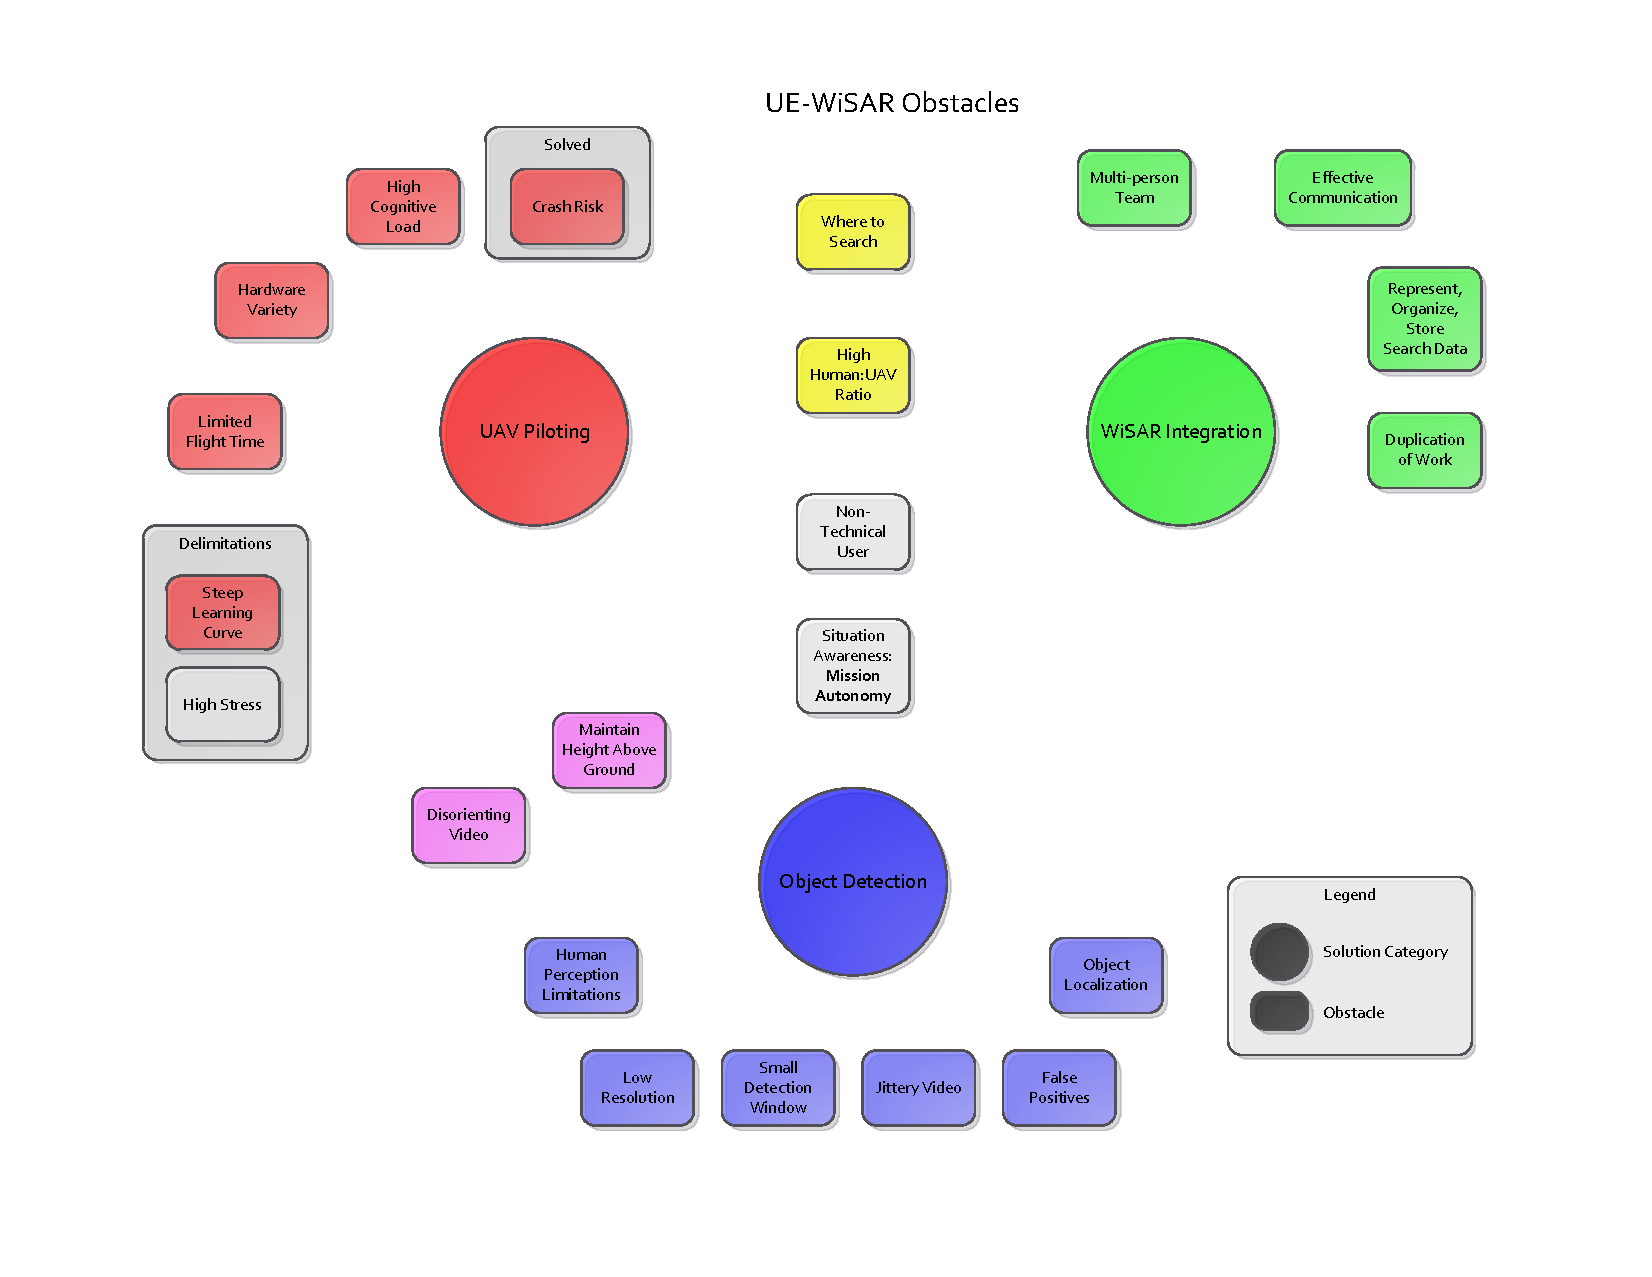
\includegraphics[keepaspectratio=true, width=\paperheight,
	height=\paperheight, page=1, angle=90, scale=0.95,
	trim=20 0 20 0]{obstacle_solution_map.pdf}
	\caption{UE-WiSAR Obstacles}
	\label{fig:obstaclemap}
\end{figure*}


\subsection{UAV Piloting}

\textbf{High Cognitive Load}.  mUAVs operate under multiple
degrees of freedom which can be disorienting for pilots.  A high level of
concentration is required to avoid becoming confused while piloting.  This is
somewhat mitigated by the low-level autonomy that this project builds upon
\cite{lin2010supporting}.  However, a fair amount of cognitive load is still
required.  Path-planning, status monitoring and team communication are tasks
that must still be addressed.

\textbf{Hardware Variety}.  The variety of hardware that can be used for mUAVs
is constantly increasing.  For any system to be viable as a perpetual framework
for UAV research it must have mechanisms in place to allow for the piloting of any number of unique mUAVs.

\textbf{Limited Flight Time}.  Most battery-powered mUAVs are limited to a
flight time of under 120 minutes, many are much less.  This limitation makes flight
planning much more difficult and introduces the potential for critical failure
during a flight.

\subsection{Object Detection}

\textbf{Human Perception Limitations}.  To be successful human
users must be able to detect objects on screen.  This implies that video presented to users
will only be effective if it accounts for the limitations of the human
eye \cite{humphrey2009human}. The eye is only able to discern high detail with
the cones located in the center.
This means that to detect an object the user must be looking almost directly at
the object while it moves across the screen.  Another limitation is that 
the eye has difficulty detecting small changes in intensity, an effect that gets
worse as brightness goes down \cite{gonzalezwoodsDIP}.

\textbf{Low Resolution}.  The video resolution is a result of
current hardware.  The mUAVs at this time broadcast NTSC 640x480 resolution. 
This resolution makes it extremely difficult to locate small objects which may be represented by only
a few pixels \cite{goodrich2009towards}.

\textbf{Small Detection Window}.  When using a fixed wing mUAV the video
captured is in constant motion.  This motion means that a potential target will
only remain visible for a short time.  Minimum mUAV flight speeds only slightly
improve the detection window and cannot fully correct this
problem \cite{goodrich2009towards}.

\textbf{Jittery Video}.  For stable flight, the mUAV is constantly correcting
course through small adjustments.  These adjustments occasionally have the
undesired effect of making video appear jittery.  This problem is magnified
in adverse weather conditions \cite{goodrich2009towards}.

\textbf{Object Localization}.  Assuming an object
has been detected in surveillance video the next step in a WiSAR operation is to send ground
searchers to the object.
In a May 2008 field trial, video analysts where unable to accurately communicate
the location of an object and had to observe the searchers from the mUAV to give
them directions relative to the object \cite{goodrich2009towards}.  This example
illustrates a different challenge which is determining the exact location of a
detected object.

\textbf{False Positive Detections}.  Due to the cost associated with missed
detection, a human life, a high false alarm rate is considered tolerable.  If
the false alarm rate is too high, however, it degrades the practicality of the
tactic.  On top of that each false alarm requires effort that may bog down the
search or leach resources from other tactics \cite{goodrich2008supporting}.

\subsection{WiSAR Integration}
The next group of obstacles fall under the WiSAR Integration category and
represent the challenges from introducing mUAVs into a WiSAR operation.
A cognitive task analysis was performed to provide
insights for such an integration  \cite{adams2009cognitive}.  The goal directed
task analysis and work domain analysis from this effort communicate how complex a
WiSAR operation is.  To integrate with such a complex endeavor a few obstacles
must be overcome.

\textbf{Multi-Person Team}.  WiSAR operations are made up
of potentially hundreds of people.  Additionally, the mUAV requires its own
team.  Not only must the mUAV team operate as a team but it must also interact
with the overall operation.  These multi-person, multi-team environments often
generate role confusion, conflict, and inefficiency
\cite{goodrich2008supporting}.

\textbf{Effective Communication}.  No search can be
effective without the relevant data.  A typical WiSAR operation uses a
hierarchical command structure.  The mUAV team must be able to fold into the
hierarchy such that it receives relevant search data.  The mUAV team must then
communicate internally as individual roles are performed.  Important information
must then be communicated back into the parent command structure.

\textbf{Representing, Organizing, and Saving Search Data}.  The data provided to
the mUAV team must be interpreted so that it can be understood by the mUAV.  Additionally the data
provided by the mUAV must then be interpreted so it can be understood by users
and commands further up the chain.  This implies an internal data organization
associated with the mUAV.  This organization must facilitate the storing and
sharing of said data.

\textbf{Duplication of Work}.  This mostly applies to search area coverage. 
The mUAV team must be able to track what it has searched and how well it
was searched.  Without this information search planning will be inaccurate which
could have fatal consequences.

\subsection{UAV Piloting \& WiSAR Integration}

\textbf{Where to Search}.  During a WiSAR
operation the probability of area (POA) \cite{koester2008lostpersons} is
constantly changing as new information is acquired.  For a UAV to integrate into
a WiSAR operation it must have the ability to interpret this information, act on
information, and contribute information.  If information is lacking then it must
be able to generate information to act upon.  A target can only be spotted by
the mUAV if it shows up on the video.

\textbf{High Human to UAV Ratios}.  This obstacle is based on practicality.  It
is not practical to require a large team for a single mUAV.
With the variety of tasks that emerge when introducing a mUAV to WiSAR it
becomes quite challenging to keep this ratio down.  A study by Cooper 
\cite{cooper2008towards, goodrich2009towards} speculates that it may be possible
for a single human to simultaneously navigate an area while localizing objects. 
His conclusion outlines several requirements he feels must be met before this
can become reality.  This becomes even more challenging when considering the
Mision Manager role as well.

\subsection{UAV Piloting \& Object Detection}
\textbf{Maintaining Height Above Ground (HAG)} \cite{adams2007camera}.
This represents one of the major crash risks associated with user error.  In an
early test flight the pilot placed two way points of similar HAG a fair distance
apart.  As the mUAV flew between the way points it crashed into a tall ridge
that separated the waypoints.  The pilot wasn't aware that his flight path went
through the ridge. This example illustrates one reason for maintaining HAG;
another reason is related to Object Detection.
Goodrich et al. state that the minimal resolution
of an image for detecting a human form is 5cm per pixel
\cite{goodrich2008supporting}.  This means that an image can cover an area no wider than
32m and 24m tall.  They go on to suggest that the
maximum HAG be between 60m to 100m.

\textbf{Disorienting Video}.  Disorienting video is produced when the mUAV is
performing manuevers which change the camera field of view and cause the user to feel
disoriented \cite{morse2008application}.  Even small manuevers can be
disorienting when occurring in succession.
This is a challenge because the UAV cannot obtain the needed surveillance
without turning.  Also, the light weight of the mUAV causes it to be
susceptible to wind which can cause excess manuevering.

\subsection{Universal Obstacles}
\textbf{Non-Technical Users}.  For UE-WiSAR to be
practical it must strive to be accessible to the greatest number of users.  With
this said UE-WiSAR is a technical operation and cannot be divorced completely
from its technical aspects.  UE-WiSAR requires some knowledge of mUAVs,
networking, and radio transmission. The real obstacle is segregating
and limiting the technical experience required for UE-WiSAR into as few roles as
possible.

\textbf{Situation Awareness}.  This represents the user's ability to maintain
awareness of the bigger picture while performing tasks.  This is broken into
two categories.  The first category relates to the mission.  The main goal of
any UE-WiSAR operation is to find the missing person.  If the tasks performed by
mUAV team members require a cognitive load that is too high team members will be
unable to meet their respective responsibilities which may have tragic
consequences to the search.  The second category relates to autonomy.  Autonomy
is a central concept to UE-WiSAR.  As autonomy increases certain negative
attributes can emerge  \cite{adams2007camera}, including:
\begin{itemize}
	\item Reduced situational awareness
	\item Difficulty in supervising autonomy
	\item Increased interaction time
	\item Increased demands on the human and autonomy
\end{itemize}
As autonomy decreases the following negative attributes
can emerge \cite{cooper2006integrating}:
\begin{itemize}
	\item High cognitive load on operator
	\item Steep learning curve
	\item Increase pilot:UAV ratio
\end{itemize}
The balancing of this dynamic relationship between the autonomous and
operator-controlled elements of UE-WiSAR is important because it is directly
linked to the usability of the solution.

\begin{figure*}[htp]
	\vspace{-80pt}
	\hspace{-90pt}
	\includegraphics[keepaspectratio=true, width=\paperheight,
	height=\paperheight, page=3, angle=90, scale=0.95,
	trim=10 0 10 0]{obstacle_solution_map.pdf}
	\caption{UAV Piloting Solutions}
	\label{fig:uavpilotingmap}
\end{figure*}

\section{SOLUTIONS}
The solutions to the above mentioned obstacles are organized into three categories.
See Figure~\ref{fig:obstaclemap} on page
\pageref{fig:obstaclemap}.  This organization is preferred because many of
the solutions discussed here solve problems associated with multiple obstacles. 

As mentioned earlier, these solutions already exist in different states.  The
subsequent paragraphs will expand on the work required to add the solution to
UE-WiSAR.

\subsection{UAV Piloting}
This solution category focuses on overcoming obstacles
associated with piloting the mUAV.  See Figure~\ref{fig:uavpilotingmap} on page
\pageref{fig:uavpilotingmap}.


% \begin{figure*}[htp]
% 	\label{fig:uavpilotingmap}
% 	\includegraphics[keepaspectratio=true,	height=1.0\textwidth, angle=90, page=3]{obstacle_solution_map.pdf}
% \end{figure*}

\textbf{Automated Flight Paths (AFP)}.  The first obstacle this addresses is the
high cognitive load on the pilot.  Detailed flight paths can be generated in a matter of
moments with minimal user input.  These flight paths can also be adjusted based
on the limited flight time.  Lin has created an algorithm
that when given a probability distribution map, start point, end point and
flight time will generate a flight path that maximizes the mUAV cameras coverage
of the probability distribution \cite{lin2009uav}.  Another type of flight path
is the Generalized Contour Search \cite{goodrich2008supporting}.  This flight
path requires a gimbaled camera but also generates optimal search patterns for certain
conditions.  Automatically generated flight paths can also attempt to limit the
number of turns made by the UAV to minimize the amount of disorienting video
captured during a flight.  Lastly, these flight paths can use HAG information to
maintain the optimal HAG for object detection while also avoiding obstacles such
as ridges or cliffs.

\textbf{Pre-Load Terrain Data}.  Terrain data provided by a number of sources
can be downloaded over the internet prior to the search.  This data is critical for
implementing effective AFPs and POA distributions.

\textbf{Modular Hardware Interface}.  To overcome the hardware variety obstacle
UE-WiSAR will use piloting interfaces that must be implemented for specific technologies.
While the initial UE-WiSAR release will have limited hardware support, namely
Procerus and Mikrocopter, more support can be added through implementing a
single interface for the specific technology.  This approach minimizes the work and knowledge required to adapt
the software to new hardware.

\textbf{UE-WiSAR Pilot UI}.  This user interface has two main
requirements \cite{lin2010supporting}.  First is assigning tasks to the mUAV. 
This implies an ability to make the mUAV an effective part of the search by
having the mUAV capture high quality video footage of regions specified by the
incident commander.  It does not imply deep understanding of mUAV piloting,
flight path automation, or other technical details associated with piloting a
mUAV \cite{cooper2007supporting}.

The second requirement is the ability to monitor the health of the mUAV.
This means the UI must communicate the exact position and status of the mUAV at
all times and alert the pilot when user input is required.  Because this UI
is the main focus point for the pilot, it is a primary concern for loss of
situation awareness.  To avoid this the UI must be able to dynamically adjust
the amount of automation needed as dictated by the situation.

\subsection{Object Detection}
This section focuses on detecting objects
in video captured by the mUAV.  See Figure~\ref{fig:objectdetectionmap} on page~\pageref{fig:objectdetectionmap}.

\begin{figure*}[htp]
	\vspace{-55pt}
	\hspace{-80pt}
	\includegraphics[keepaspectratio=true, width=\paperheight,
	height=\paperheight, page=4, angle=90, scale=0.90,
	trim=20 0 20 0]{obstacle_solution_map.pdf}
	\caption{UAV Piloting Solutions}
	\label{fig:objectdetectionmap}
\end{figure*}
% \begin{figure*}[htp]
% 	\label{fig:objectdetectionmap}
% 	\includegraphics[keepaspectratio=true,	height=1.0\textwidth, angle=90, page=4]{obstacle_solution_map.pdf}
% \end{figure*}

\textbf{Temporally Localized Mosaic} \cite{morse2008application,
cluff2009unified}.  This process allows the user to view the current frame in relation to a history of previous frames.  An object that appeared in a
single frame may now remain visible for multiple frames.  Morse et al. conducted
user studies to analyze the effectiveness of this
approach.  Those studies found a 43\% improvement in
hit probability when using mosaiced views versus non-mosaiced views.  While
there was an increase in false positive detections this increase is considered
inconsequential along side the improvement to hit probability.

\textbf{Spectral Anomaly Detection} \cite{thornton2011detection,
rasmussen2008enhancement}.  In typical WiSAR video the majority of colors are
varying shades of grey, brown, and green.  This process looks for objects that
are ``out-of-place''.  This autonomous detection will not replace user
detection, instead it aids user detection by suggesting objects to the user for
closer inspection.

\textbf{GPS Frame Referencing} \cite{morse2010coverage}.  This process uses
geometry to map pixels to gps coordinates.  The
algorithm uses the GPS coordinates of the mUAV, mUAV position, terrain data,
and camera specifications to determine the relation of the point to the UAV. 
While the process is simple, it suffers from the limited precision of mUAV
sensors and may provide highly inaccurate locations.

\textbf{Video Analyst UI} \cite{lin2010supporting}.  This UI is meant for users
operating under the Video Analyst Role.  Its purpose is to help Video
Analysts detect objects seen by the mUAV.  There are three main requirements
associated with accomplishing this purpose.  The first is to provide video to
the user.  As a search progresses Video Analysts may need to analyze live video,
video of specific areas, or video from certain times.  The UI must make it easy
for analysts to find the video that needs to be analyzed.  The second
requirement is to aid in object detection.  The UI must be able to enhance the
video as directed by the user.  This includes the above mentioned solutions
along with other simple enhancements such as brightness, contrast, and rate of
playback.  The last requirement is that the UI allow the analyst to communicate
with the mUAV team.  As an analyst works they must be able to communicate
findings to the mUAV team.

\subsection{WiSAR Integration}
WiSAR Integration focuses on introducing a mUAV to a
WiSAR operation.  See Figure~\ref{fig:wisarintegrationmap} on
page~\pageref{fig:wisarintegrationmap}.

\begin{figure*}[htp]
	\vspace{-90pt}
	\hspace{-80pt}
	\includegraphics[keepaspectratio=true, width=\paperheight,
	height=\paperheight, page=2, angle=90, scale=0.95,
	trim=10 0 10 0]{obstacle_solution_map.pdf}
	\caption{WiSAR Integration}
	\label{fig:wisarintegrationmap}
\end{figure*}
% \begin{figure*}[htp]
% 	\label{fig:wisarintegrationmap}
% 	\includegraphics[keepaspectratio=true,	height=1.0\textwidth, angle=90, page=2]{obstacle_solution_map.pdf}
% \end{figure*}

\textbf{Team Roles} \cite{goodrich2008supporting,adams2009cognitive,goodrich2007using}.  UE-WiSAR will use a hierarchical command structure.
The top level role is the \emph{Mission Manager} (MM).  The MM is responsible
for defining the search in UE-WiSAR.  The MM is also responsible for directing
the other roles associated with a mUAV search.

The next role is \emph{UAV Pilot}.  The Pilot is responsible for capturing video with the
mUAV as directed by the MM and communicating important information about the
status of the mUAV to the MM.  

The last role is \emph{Video Analyst}.  The
Analyst is responsible for detecting objects in the captured video.
The Analyst communicates any findings to the MM.  

This role breakdown enables a
mUAV team of two or more people to operate effectively through a clean breakdown
of work and established communication channels.

\textbf{Independent Technical Search Team}
\cite{adams2009cognitive}.
UE-WiSAR represents a single search tactic for locating missing persons.  This
implies that UE-WiSAR will be used as part of a larger WiSAR operation.  This is
facilitated through the MM role.
The MM is responsible for obtaining the missing person data and entering the
data into UE-WiSAR.  The MM is then responsible for constructing a mUAV search
plan as directed from the chain of command.  As the mUAV team follows the
search plan, everything is reported back to the MM who then relays relevant
information back to the main chain of command.

\textbf{Command \& Control UI} This UI is meant for users operating under the
Mission Manager Role.  Its purpose is to facilitate the MM responsibilities. 
There are three main requirements for accomplishing this purpose.  The first is the ability to build a missing person profile. 
Information such as the last known location, clothing color, destination,
starting point, etc. is essential for the automation and the mUAV team. 
The UI must allow the MM to enter this data but not overload the MM with tedious
data entry.  The next requirement is the ability to define a search plan.  The
UI must show relevant search data to the MM and allow the MM to define a search
plan which can then be carried out by the Pilot.  The
last requirement is the ability to receive communications from mUAV team members.  The UI must alert the
IC of detected objects, mUAV status, search progress.  The UI must also
communicate this information in a way that it can be presented to the main chain
of command.  Additionally the UI must be intuitive, clean, and simple.

\textbf{Distributed System Design}  A client-server architecture has been chosen
for UE-WiSAR for several reasons.  The first reason is the computational load
required to enhance video received by the mUAV.  The resources needed are much
greater than those of a typical desktop computer and require a powerful server. 
Once the video has been enhanced, however, it can be distributed to clients at
little cost.  Another reason for this architecture is the unknown team size. 
Collected video must be analyzed by the human-eye.  This architecture allows for
any number of video analysts to work symultaneously, assuming there is enough bandwidth.
Another reason for this architecture is to simplify the software.  Instead of
building an all-in-one software solution, a server and multiple independent
client applications can be written.  Clients can then choose which application
to run according to their roles which in turn makes the client roles less
confusing.

\textbf{Video Annotations}  These are the primary means of communication for the
Analysts.  When an Analyst detects an object they can click on the object and
create an annotation.  The annotation will then carry information about that
object such as location, time of discovery, place in video, analyst comments,
priority, etc.  Once an annotation is created it instantly becomes
available to other team members, in the case of the IC, alerting them of the
annotation.  The annotation can then be modified as needed depending if it was a
false alarm or a real sign.  If an annotation is a real sign it can be converted
to a format acceptable to the external chain of command.

\textbf{Persistent Incident Management}  Essentially this refers to a relational
data model specifically designed for UE-WiSAR.  The root node of this data model
will be an incident, all other data will be linked to an incident.  The model
will hold missing person data, search plans, flight plans, videos, annotations,
etc.  Storing data in the model will reduce work duplication and make
data more accessible.  The model will also simplify persistent storage as xml
files or a sql database.  In concert with the project goals this data model can
be shared with other search groups and search databases to help improve WiSAR.

\textbf{See-Ability} \cite{engh2008see}  This is a method of determining how
well an area has been searched by the mUAV.  The algorithm uses the position of the
camera in relation to the ground to determine the quality of the view.  This can
later be used to find how many times a location has been viewed, how many unique
angles has it been viewed from, and what is the overall quality of the viewings.
This can be a great help to the MM and Pilot in avoiding over-viewed areas,
narrowing search parameters, and maintaining situation awareness.

\textbf{POA Models} \cite{koester2008lostpersons}  Because UE-WiSAR must
be able to act independently, two probability of area models will be added
to the CC interface.  The first is the Segment Model.  This model allows the IC
to strategically breakdown a large search region into smaller search regions. 
Efforts can then be focused on high priority regions as directed by the IC.  The
second model is the Ring/Dispersion Model.  This model uses the last known
location along with the intended destination to create an ever expanding search
corridor with eminating rings that occur at specific distances.  The
highest POA occurs inside the corridor and inside the first ring, then second
ring, etc.


\section{DELIVERABLES}
As an industrial thesis a major goal is to produce high quality software that is
on par with industry standards.  Quality as it relates to the project goals is
the users ability to perform tasks within their roles and to allow future
developers to understand UE-WiSAR well enough to modify/enhance the software as
needed.  To following descriptions of work will be used to validate that the
project goals have been met and that the project is a success.

Therefore, the first deliverable will be a detailed list of requirements
organized into groups and prioritized.  Glass's law states that ``Requirement deficiencies are the prime source of project failures.''  The list of requirements is meant to be an ideal goal.
Not every requirment will be acheived, and some may change, instead it is meant
to be a road map.  By clarifying the project requirements early the student and
committee members can make informed decisions, avoid mistakes, and measure progress.
It is also expected that design specifications will improve the design and make
prototyping more effective.  

The second deliverable will be detailed design documents specifying the
architecture, data model, workflows, dataflows, protocols, user manuals and
language/framework considerations.  These documents will make up a collection
of text, UML, and other documents.  Their purpose is to clarify how the system
works and how it accomplishes project goals.  Boehm's first law states ``Errors are most frequent during the requirements and design activities and are the
more expensive the later they are removed."  This step of the project will help
to reduce bugs and development time by allowing for peer review and prototyping
before major work is done.  Many of these documents are living documents and
will change as the project progresses, some may not exist until after coding
has been completed.  It is expected that requirements and design will take up to
one third of the total project time.

The third deliverable will be the actual UAV Enabled Wilderness Search and
Rescue code.  The code will be well documented, follow consistent coding
practices, and compile on designated operating systems.  This represents the
majority of work done on the project.

The fourth deliverable will be a demonstration of the software in a
live environment with a real mUAV and controlled targets.  This demostration
will show that core features exist, the software is stable, and users are able to perform tasks by following written
instructions.  Core features are the set of features decided on by the student
and committee that the software must have to be considered functional.  The
users will be individuals, preferably familiar with WiSAR, unfamiliar with
operating the UE-WiSAR software.  At least one user per role will be involved. 
An experienced mUAV pilot will also be involved to reduce risk to equipment. 
Basic tasks will be assigned that require use of the core features.  This will
not be an exercise in validating prior research.

% \section{Specification of Work}
% As mentioned, a substantial amount of work has already been done in
% consolidating the prototype code and implementing the proposed project.  The
% current WonderServer project, developed in C++ on the QT framework, has a
% Server, Pilot UI, and Video Analyst UI \cite{uavCode, serverCode}.  While each
% component is incomplete, stable network communication, open GL integration, and mUAV Hardware communication are working.  The ability
% to perform these basic tasks proves the capability of the chosen framework.  The
% next step is to engineer the software to maximize the potential to fulfill its
% goals.  The Model View Controller (MVC) design pattern will represent the
% overall design.  This is ideal because UE-WiSAR has a minimum of four UIs that will all
% interact with the same Model.  To fit UE-WiSAR to the MVC pattern the following
% tasks must be completed.
% 
% \textbf{Data Model}  A Data Model will be designed to store information for a
% WiSAR incident.  All data that is relevent to the system will be represented in
% the Data Model.  The model will be responsible for assigning unique id's to
% objects and maintaining data integrity of the objects it stores.  To simplify
% model interaction the Facade pattern will be used both in and around the model
% wherever the logic becomes moderately complex.  The model will use appropriate
% design patterns to represent the data.
% 
% \textbf{Data Persistence}  Beneath the Model layer a Data Persistence layer will
% exist that can convert the Model into a persistent medium.  Initially this will
% be as serialized data files, however, the design allows for the addition of
% other mediums such as SQL without impacting the system.
% 
% \textbf{Controllers}  The controllers are responsible for communicating between
% the Model and the View.   Because the View can be on a different machine than
% the Model this communication is more complex.  Views will be expected to
% maintain their own custom models.  The controller will be responsible for
% syncing the data in these models as necessary.  A client controller will
% interact with a sibling controller on the server as needed through a network
% interface.  Interfaces must be created for all Controllers before the
% controllers are created.
% 
% \textbf{Views}  Interfaces must be created for all Views before the Views are
% created.  Each UI is made up of one or more Views and can become confusing. 
% Interfaces are pre-designed so that when implemented will ensure all required
% features are met.  A general idea of the requirements for each view are as
% follows:
% 
% \begin{itemize}
% 	\item \textbf{Server}
% 	\begin{itemize}
% 	  \item Add/Edit mUAV Hardware Connections
% 	  \item Add/Edit an Incident
% 	  \item View Terrain Data
% 	  \item View Video
% 	\end{itemize}
% 	
% 	\item \textbf{Command \& Control UI}
% 	\begin{itemize}
% 	  \item Add/Edit an Incident
% 	  \item Add/Edit POA Models
% 	  \item View Terrain Data
% 	  \item View See-Ability
% 	  \item View Annotations
% 	  \item View Video
% 	\end{itemize}
% 	
% 	\item \textbf{Pilot UI}
% 	\begin{itemize}
% 	  \item Add/Edit mUAV Hardware Connections
% 	  \item Add/Edit Flight Paths
% 	  \item View Terrain Data
% 	  \item View Search Areas
% 	  \item View Annotations
% 	  \item View mUAV Status
% 	  \item View Live Video
% 	\end{itemize}
% 	
% 	\item \textbf{Video Analyst UI}
% 	\begin{itemize}
% 	  \item View Video
% 	  \item Add/Edit Annotations
% 	  \item View Incident Information
% 	\end{itemize}
% \end{itemize}
% 
% There is also work that must be done outside of the MVC structure.  Most of the
% autonomous solutions that will be implemented integrate with the Data Model,
% however, they exist separate from the MVC design.
% These solutions will be implemented as independent libraries that will be used
% by the Data Model and Controllers as needed.  An example of this is Automatic
% Flight Path Generation, Mosaicing, Anomoly Detection, etc.  The status of
% these libraries was described previously.

% \subsection{Time to Complete}
% An important concern is the time to complete this project.  It is possible that
% not everything can be coded in the time alloted.  With this consideration it is
% important to recognize what aspects of the software are required to consider the
% project a success.  
% 
% The first of the requirements is the porting of prototype code into individual
% QT libraries.  These libraries represent the intelligence and automation behind
% the UE-WiSAR software and are a major part of the research done here at BYU. 
% This includes but is not limited to Mosaicing, See-Ability, Anomoly Detection,
% Flight Path Generation, POA Modeling, and UAV communication.
% 
% The second requirement is the UE-WiSAR Server.  The server is responsible
% for collecting and storing data from mUAVs, Video Streams, External Map
% Sources, GUI's, and UE-WiSAR clients.  As data comes in from these sources the
% server uses the above mentioned libraries to extrapolate more data.  This is the
% backbone of the UE-WiSAR project and must be completed.  For detailed
% requirements look at 
% 
% The last requirement to mark the project successful is for user validation of
% the features described in this proposal.  This represents the CC, Pilot, and
% Video Analyst Clients.  These clients must be developed enough that a user
% familiar to WiSAR can perform a search and verify that the described features
% exist and work.  The user interfaces will be what suffer the most if time
% becomes short.  The reason this is acceptable is because the clients implement the Controller and View interfaces
% which make them easily replaceable.  New GUI's can be created as needed that
% implement the same interfaces but which look and feel much more polished with
% little to no consideration to backend operation.  In fact it is expected that
% when released most community contributions will be in the form of GUI
% enhancements.

% \section{Validation}
% There are two aspects to the validation of the project.  The first is validation
% of the quality of the software.  As an industrial thesis a major goal is to
% produce software that is on par with industry standards.  This will be
% accomplished through documentation.  Comments will be included on each class
% that describe the purpose of the class and what it does.  Using Doxygen this
% data will be compiled into detailed class documents.  Also, design documents
% describing the Data Model, Design Patterns, WiSAR Integration and Usage of key
% features will be created.
% 
% The second validation aspect will be the verification of the minimum set of
% requirements.  Monthly design review meetings will be held, if needed the
% requirements can be modified in these meetings.  The minimum list of
% requirements will be verified by an individual familiar with the UE-WiSAR
% software.  If the user can perform the minimum requirement list then the
% software will be considered validated.  See Figure~\ref{fig:serverrequirements}
% on page~\pageref{fig:serverrequirements}.
% 
% \begin{figure*}[htp]
% 	\caption{Detailed Server Requirements}
% 	\begin{itemize}
% 		\item \textbf{Incident Information}
% 		\begin{itemize}
% 		  	\item Manage Search Incidents
% 		  	\begin{itemize}
% 			  	  \item Incident Area
% 			  	  \item Missing Person Profile
% 			  	  \item Last Known Locations
% 	  	  	\end{itemize}
% 	  	  	\item Load existing Search Incidents
% 	  	  	\item Switch between Incidents
% 	  	  	\item Generate POA models from Missing Person Data
% 	  	  	\item Automatically Download Terrain Data for Incident Area
% 		\end{itemize}
% 		
% 		\item \textbf{Terrain Data}
% 		\begin{itemize}
% 			\item Obtain Third Party Map Data for a specified incident area.
% 	  		\begin{itemize}
% 	  		  	\item MapQuest Image Tiles
% 	  		  	\item OpenMaps Image Tiles
% 	  		  	\item USGS NED 1/3 GridFloat
% 	  		  	\item USGS LandCover GridFloat
% 		  	\end{itemize}
% 		  	\item Save Terrain Data to disk
% 		  	\item Make Terrain Data available to clients
% 		  	\item Perform fast queries on Terrain Data
% 	  		\begin{itemize}
% 	  		  	\item HAG of specific coordinate
% 	  		  	\item LandCover of specific coordinate
% 		  	\end{itemize}
% 	  		\item Manage Incident Map Objects
% 			\begin{itemize}
% 			  \item Points
% 			  \item Areas
% 			  \item Custom Objects
% 			\end{itemize}
% 		\end{itemize}
% 		
% 		\item \textbf{Video}
% 		\begin{itemize}
% 	  		\item Manage Camera Profiles
% 	  		\item Capture Video Frames
% 	  		\begin{itemize}
% 	  	 		\item Save Frames to Harddrive
% 	  	  		\item Save GPS Location of Frame
% 	  	  		\item Connect Frame to Incident
% 	  	  		\item Homography Calculation on Frame
% 	  	  		\item Anomoly Analysis on Frame
% 	  		\end{itemize}
% 		  	\item Stream Captured Video
% 		  	\item Manage Annotations
% 		\end{itemize}
% 		
% 		\item \textbf{UAV}
% 		\begin{itemize}
% 		  	\item Manage UAV Profiles
% 		  	\item Manage UAV Plugins
% 		  	\item Communicate with UAV
% 		  	\begin{itemize}
% 		  	  	\item Save UAV data to Harddisk
% 		  	  	\item Issue Commands to UAV
% 		  	  	\item Track UAV position
% 	  	  	\end{itemize}
% 	  	  	\item Generate Flight Paths
% 	  	  	\item Monitor UAV Status
% 	  	  	\item Manage See-Ability
% 		\end{itemize}
% 	\end{itemize}
% 	
% 	\label{fig:serverrequirements}
% \end{figure*}
\section{DELIMITATIONS}
Due to the nature of software development and the size of this project there
will be a large list of things to do that can be done in a reasonable amount of
time.  The goal of this project is not to implement the maximum amount of
features, instead the goal is to create a stable foundation for others to
implement the features they choose.  This is particularly relevent in regards to
user interfaces.  

This project will not create the ideal user interfaces as described in the
solution section as those are subjective and become much too time consuming. 
Instead the project will focus on functionality and creating basic user interfaces that can be
easily replaced by future developers.

The project also doesn't account for the High Stress that is associated with SAR
operations.  It is known that High Stress has a negative impact on an
individuals cognitive load capacity, however, it is too complicated to include in this proposal.  

There are several learning curves that are associated
with different aspects of this project.  Because learning curves are unavoidable
and vary with the individual it is enough for this proposal that the software is
targeted at as large a user group as possible.

There are too many unknowns to accurately predict the amount of time a project
this size will take to complete.  The focus will be on the deliverables and
working closely with advisors during the development process to adjust the
requirements to fit with time constraints.

\section{CONCLUSION}
UE-WiSAR represents an opportunity for the research done at BYU to serve a
greater community.  As Thomas Edison once said ``The value of an idea lies in
the using of it.''  UE-WiSAR will not only provide a new search Tactic for
SAR operations, it also provides a framework for mUAV enthusiasts and
researchers to build upon for continued research in the field.  What now exists
as a collection of interesting ideas will become the do-it-yourself manual for
performing aerial surveillance using mUAVs.  

Unlike many open source solutions, the focus of creating software at current
industry standards makes UE-WiSAR even more valuable.  With good design and
documentation the project is much more likely to take hold in the open source
community further increasing its ability to serve those communities it is meant
to serve.
\chapter{Code and Models} \label{code}

The source code for the modeling framework, xml parsing, WiSAR model, and UAS integration into the NAS models can be obtained on github from the following link:

\url{https://github.com/tjflexmaster/UAV_ROLE_MODEL}
\chapter{Debug Log Generated by the Model}

This is the output log generated when running the UAS integrated into the NAS model with automatic emergency NOTAM avoidance.  The main simulation cycle consists of three main parts: Load transitions, advance time, and fire transitions.


\begin{spacing}{1}
\tiny
\begin{verbatim}
Load Transition(1):	 Start a new UAV mission
Time: 1
Fired Transition:	 Start a new UAV mission
-----------------------------------------------
Load Transition(1):	UAVOP: StartState: IDLE EndState: BUILD_FP Description: Received new mission, begin building flight plan.
Time: 2
Fired Transition:	UAVOP: StartState: IDLE EndState: BUILD_FP Description: Received new mission, begin building flight plan.
-----------------------------------------------
Load Transition(900):	UAVOP: StartState: BUILD_FP EndState: BUILD_FP Description: Build a flight plan
Time: 902
Fired Transition:	UAVOP: StartState: BUILD_FP EndState: BUILD_FP Description: Build a flight plan
-----------------------------------------------
Load Transition(1):	UAVOP: StartState: BUILD_FP EndState: END_BUILD_FP Description: Click the Send flight plan button
Time: 903
Fired Transition:	UAVOP: StartState: BUILD_FP EndState: END_BUILD_FP Description: Click the Send flight plan button
-----------------------------------------------
Load Transition(1):	UAS: StartState: NORMAL EndState: NORMAL Description: Send flight plan to FAA
Load Transition(1):	UAVOP: StartState: END_BUILD_FP EndState: WAITING_ON_FAA Description: Clear mouse and keyboard output layers
Time: 904
Fired Transition:	UAS: StartState: NORMAL EndState: NORMAL Description: Send flight plan to FAA
Fired Transition:	UAVOP: StartState: END_BUILD_FP EndState: WAITING_ON_FAA Description: Clear mouse and keyboard output layers
-----------------------------------------------
Load Transition(1):	FAA: StartState: NORMAL EndState: NORMAL Description: Received Flight plan from UAS
Time: 905
Fired Transition:	FAA: StartState: NORMAL EndState: NORMAL Description: Received Flight plan from UAS
-----------------------------------------------
Load Transition(1):	ATC: StartState: NORMAL EndState: APPROVING_FLIGHT_PLAN Description: ATC is ready to approve flight plans.
Time: 906
Fired Transition:	ATC: StartState: NORMAL EndState: APPROVING_FLIGHT_PLAN Description: ATC is ready to approve flight plans.
-----------------------------------------------
Load Transition(200):	ATC: StartState: APPROVING_FLIGHT_PLAN EndState: END_APPROVING_FLIGHT_PLAN Description: ATC is approving flight plans.
Time: 1106
Fired Transition:	ATC: StartState: APPROVING_FLIGHT_PLAN EndState: END_APPROVING_FLIGHT_PLAN Description: ATC is approving flight plans.
-----------------------------------------------
Load Transition(1):	ATC: StartState: END_APPROVING_FLIGHT_PLAN EndState: NORMAL Description: ATC finished approving the flight plan.
Load Transition(1):	FAA: StartState: NORMAL EndState: NORMAL Description: FAA received approved flight plan from ATC, send to UAS
Time: 1107
Fired Transition:	ATC: StartState: END_APPROVING_FLIGHT_PLAN EndState: NORMAL Description: ATC finished approving the flight plan.
Fired Transition:	FAA: StartState: NORMAL EndState: NORMAL Description: FAA received approved flight plan from ATC, send to UAS
-----------------------------------------------
Load Transition(1):	UAS: StartState: NORMAL EndState: NORMAL Description: Received flight plan approved from FAA
Time: 1108
Fired Transition:	UAS: StartState: NORMAL EndState: NORMAL Description: Received flight plan approved from FAA
-----------------------------------------------
Load Transition(30):	UAVOP: StartState: WAITING_ON_FAA EndState: END_WAITING_ON_FAA Description: FAA approved the flight
Time: 1138
Fired Transition:	UAVOP: StartState: WAITING_ON_FAA EndState: END_WAITING_ON_FAA Description: FAA approved the flight
-----------------------------------------------
Load Transition(1):	UAS: StartState: NORMAL EndState: NORMAL Description: UAVOP sent take off command
Load Transition(1):	UAVOP: StartState: END_WAITING_ON_FAA EndState: MONITOR_TAKEOFF Description: Clear user output
Time: 1139
Fired Transition:	UAS: StartState: NORMAL EndState: NORMAL Description: UAVOP sent take off command
Fired Transition:	UAVOP: StartState: END_WAITING_ON_FAA EndState: MONITOR_TAKEOFF Description: Clear user output
-----------------------------------------------
Load Transition(1):	UAV: StartState: GROUNDED EndState: TAKEOFF Description: Move to takeoff from UAVGUI cmd
Time: 1140
Fired Transition:	UAV: StartState: GROUNDED EndState: TAKEOFF Description: Move to takeoff from UAVGUI cmd
-----------------------------------------------
Load Transition(300):	UAV: StartState: TAKEOFF EndState: FLYING Description: Automatic Transition to Flying
Load Transition(1):	UAS: StartState: NORMAL EndState: NORMAL Description: UAV has started to takeoff, show this to the UAVOp
Time: 1141
Fired Transition:	UAS: StartState: NORMAL EndState: NORMAL Description: UAV has started to takeoff, show this to the UAVOp
-----------------------------------------------
Time: 1440
Fired Transition:	UAV: StartState: TAKEOFF EndState: FLYING Description: Automatic Transition to Flying
-----------------------------------------------
Load Transition(1):	Potential collision on UAS radar
Load Transition(1):	FAA radar shows a potential collision with a UAV
Load Transition(1):	Request that ATC create a new NOTAM on UAV FP
Load Transition(10000):	UAV: StartState: FLYING EndState: LANDING Description: UAV normal flight
Load Transition(1):	UAS: StartState: NORMAL EndState: NORMAL Description: UAV has started to fly, show this to the UAVOp
Load Transition(1):	UAVOP: StartState: MONITOR_TAKEOFF EndState: MONITOR_UAVGUI Description: UAV is airborne, move to monitor GUI
Time: 1441
Fired Transition:	Request that ATC create a new NOTAM on UAV FP
Fired Transition:	Potential collision on UAS radar
Fired Transition:	UAS: StartState: NORMAL EndState: NORMAL Description: UAV has started to fly, show this to the UAVOp
Fired Transition:	FAA radar shows a potential collision with a UAV
Fired Transition:	UAVOP: StartState: MONITOR_TAKEOFF EndState: MONITOR_UAVGUI Description: UAV is airborne, move to monitor GUI
-----------------------------------------------
Load Transition(1):	ATC: StartState: NORMAL EndState: CREATE_NOTAM Description: ATC needs to create a new NOTAM
Load Transition(1):	FAA: StartState: NORMAL EndState: NORMAL Description: Potential collision on FAA Radar, show the user
Load Transition(1):	UAS: StartState: NORMAL EndState: NORMAL Description: UAS received radar collision event
Load Transition(900):	UAVOP: StartState: MONITOR_UAVGUI EndState: MONITOR_UAVGUI Description: Monitoring the UAVGUI
Time: 1442
Fired Transition:	ATC: StartState: NORMAL EndState: CREATE_NOTAM Description: ATC needs to create a new NOTAM
Fired Transition:	FAA: StartState: NORMAL EndState: NORMAL Description: Potential collision on FAA Radar, show the user
Fired Transition:	UAS: StartState: NORMAL EndState: NORMAL Description: UAS received radar collision event
-----------------------------------------------
Load Transition(1):	ATC: StartState: CREATE_NOTAM EndState: CREATE_EMERGENCY_NOTAM Description: ATC sees the alert about a UAV collision and tries to avoid it
Load Transition(1):	UAVOP: StartState: MONITOR_UAVGUI EndState: AVOID_COLLISION Description: Operator sees a potential conflict and trys to avoid it
Time: 1443
Fired Transition:	ATC: StartState: CREATE_NOTAM EndState: CREATE_EMERGENCY_NOTAM Description: ATC sees the alert about a UAV collision and tries to avoid it
Fired Transition:	UAVOP: StartState: MONITOR_UAVGUI EndState: AVOID_COLLISION Description: Operator sees a potential conflict and trys to avoid it
-----------------------------------------------
Load Transition(60):	ATC: StartState: CREATE_EMERGENCY_NOTAM EndState: END_CREATE_EMERGENCY_NOTAM Description: ATC is creating an Emergency Notam around the collision
Load Transition(300):	UAVOP: StartState: AVOID_COLLISION EndState: AVOID_COLLISION Description: Operator is in the act of deconflicing the UAV
Time: 1503
Fired Transition:	ATC: StartState: CREATE_EMERGENCY_NOTAM EndState: END_CREATE_EMERGENCY_NOTAM Description: ATC is creating an Emergency Notam around the collision
-----------------------------------------------
Load Transition(1):	ATC: StartState: END_CREATE_EMERGENCY_NOTAM EndState: AVOID_UAV_COLLISION Description: ATC is creating an Emergency Notam around the collision
Load Transition(1):	FAA: StartState: NORMAL EndState: NORMAL Description: ATC sent an Emergency NOTAM to the FAA system, send it to the UAS
Time: 1504
Fired Transition:	ATC: StartState: END_CREATE_EMERGENCY_NOTAM EndState: AVOID_UAV_COLLISION Description: ATC is creating an Emergency Notam around the collision
Fired Transition:	FAA: StartState: NORMAL EndState: NORMAL Description: ATC sent an Emergency NOTAM to the FAA system, send it to the UAS
-----------------------------------------------
Load Transition(500):	ATC: StartState: AVOID_UAV_COLLISION EndState: AVOID_UAV_COLLISION Description: ATC is waiting for collision to stop.
Load Transition(1):	UAS: StartState: NORMAL EndState: NORMAL Description: Receive Emergency Notam on the UAV, force UAV away from NOTAM
Time: 1505
Fired Transition:	UAS: StartState: NORMAL EndState: NORMAL Description: Receive Emergency Notam on the UAV, force UAV away from NOTAM
-----------------------------------------------
Load Transition(1):	UAV: StartState: FLYING EndState: AVOID_NOTAM Description: UAV gets a command to avoid a NOTAM
Time: 1506
Fired Transition:	UAV: StartState: FLYING EndState: AVOID_NOTAM Description: UAV gets a command to avoid a NOTAM
-----------------------------------------------
Load Transition(300):	UAV: StartState: AVOID_NOTAM EndState: LOITER Description: Avoid the Emergency NOTAM
Load Transition(1):	UAS: StartState: NORMAL EndState: NORMAL Description: UAV is avoiding a NOTAM, show this to the UAVOp
Time: 1507
Fired Transition:	UAS: StartState: NORMAL EndState: NORMAL Description: UAV is avoiding a NOTAM, show this to the UAVOp
-----------------------------------------------
Time: 1743
Fired Transition:	UAVOP: StartState: AVOID_COLLISION EndState: AVOID_COLLISION Description: Operator is in the act of deconflicing the UAV
-----------------------------------------------
Load Transition(1):	UAS: StartState: NORMAL EndState: NORMAL Description: Radar collision has been avoided
Time: 1744
Fired Transition:	UAS: StartState: NORMAL EndState: NORMAL Description: Radar collision has been avoided
-----------------------------------------------
Load Transition(1):	UAVOP: StartState: AVOID_COLLISION EndState: MONITOR_UAVGUI Description: Collision has been avoided, return to watching the UAVGUI
Time: 1745
Fired Transition:	UAVOP: StartState: AVOID_COLLISION EndState: MONITOR_UAVGUI Description: Collision has been avoided, return to watching the UAVGUI
-----------------------------------------------
Load Transition(1):	UAVOP: StartState: MONITOR_UAVGUI EndState: AVOID_EMERGENCY_NOTAM Description: Operator notices an emergency notam on the UAV and attempts to assist
Time: 1746
Fired Transition:	UAVOP: StartState: MONITOR_UAVGUI EndState: AVOID_EMERGENCY_NOTAM Description: Operator notices an emergency notam on the UAV and attempts to assist
-----------------------------------------------
Load Transition(300):	UAVOP: StartState: AVOID_EMERGENCY_NOTAM EndState: AVOID_EMERGENCY_NOTAM Description: Operator is waiting for the UAV to auto remove itself from the Emergency Notam
Time: 1806
Fired Transition:	UAV: StartState: AVOID_NOTAM EndState: LOITER Description: Avoid the Emergency NOTAM
-----------------------------------------------
Load Transition(1):	End the FAA potential collision with a UAV
Load Transition(10000):	UAV: StartState: LOITER EndState: LANDING Description: Default to land after loitering for a long time.
Load Transition(1):	UAS: StartState: NORMAL EndState: NORMAL Description: UAV is now Loitering, show this to the UAVOp
Time: 1807
Fired Transition:	End the FAA potential collision with a UAV
Fired Transition:	UAS: StartState: NORMAL EndState: NORMAL Description: UAV is now Loitering, show this to the UAVOp
-----------------------------------------------
Load Transition(1):	FAA: StartState: NORMAL EndState: NORMAL Description: Radar collision has ended.
Load Transition(5):	UAVOP: StartState: AVOID_EMERGENCY_NOTAM EndState: AVOID_EMERGENCY_NOTAM Description: Operator sees that the UAV is loitering, have it resume flight now.
Time: 1808
Fired Transition:	FAA: StartState: NORMAL EndState: NORMAL Description: Radar collision has ended.
-----------------------------------------------
Load Transition(1):	ATC: StartState: AVOID_UAV_COLLISION EndState: NORMAL Description: FAA radar no longer shows a potential collision
Time: 1809
Fired Transition:	ATC: StartState: AVOID_UAV_COLLISION EndState: NORMAL Description: FAA radar no longer shows a potential collision
-----------------------------------------------
Load Transition(1):	ATC: StartState: NORMAL EndState: CREATE_NOTAM Description: ATC needs to create a new NOTAM
Time: 1810
Fired Transition:	ATC: StartState: NORMAL EndState: CREATE_NOTAM Description: ATC needs to create a new NOTAM
-----------------------------------------------
Load Transition(60):	ATC: StartState: CREATE_NOTAM EndState: END_CREATE_NOTAM Description: ATC is creating a new NOTAM
Time: 1812
Fired Transition:	UAVOP: StartState: AVOID_EMERGENCY_NOTAM EndState: AVOID_EMERGENCY_NOTAM Description: Operator sees that the UAV is loitering, have it resume flight now.
-----------------------------------------------
Load Transition(1):	UAS: StartState: NORMAL EndState: NORMAL Description: UAVOP sent resume flight
Load Transition(1):	UAVOP: StartState: AVOID_EMERGENCY_NOTAM EndState: MONITOR_UAVGUI Description: NOTAM has been avoided, return to watching the UAVGUI
Time: 1813
Fired Transition:	UAS: StartState: NORMAL EndState: NORMAL Description: UAVOP sent resume flight
Fired Transition:	UAVOP: StartState: AVOID_EMERGENCY_NOTAM EndState: MONITOR_UAVGUI Description: NOTAM has been avoided, return to watching the UAVGUI
-----------------------------------------------
Load Transition(1):	UAV: StartState: LOITER EndState: FLYING Description: Resume a normal flight
Time: 1814
Fired Transition:	UAV: StartState: LOITER EndState: FLYING Description: Resume a normal flight
-----------------------------------------------
Load Transition(10000):	UAV: StartState: FLYING EndState: LANDING Description: UAV normal flight
Load Transition(1):	UAS: StartState: NORMAL EndState: NORMAL Description: UAV has started to fly, show this to the UAVOp
Time: 1815
Fired Transition:	UAS: StartState: NORMAL EndState: NORMAL Description: UAV has started to fly, show this to the UAVOp
-----------------------------------------------
Load Transition(900):	UAVOP: StartState: MONITOR_UAVGUI EndState: MONITOR_UAVGUI Description: Monitoring the UAVGUI
Time: 1870
Fired Transition:	ATC: StartState: CREATE_NOTAM EndState: END_CREATE_NOTAM Description: ATC is creating a new NOTAM
-----------------------------------------------
Load Transition(1):	ATC: StartState: END_CREATE_NOTAM EndState: NORMAL Description: ATC finished creating NOTAM return to normal
Load Transition(1):	FAA: StartState: NORMAL EndState: NORMAL Description: FAA received new NOTAM on UAV FP from ATC, send to UAS
Time: 1871
Fired Transition:	ATC: StartState: END_CREATE_NOTAM EndState: NORMAL Description: ATC finished creating NOTAM return to normal
Fired Transition:	FAA: StartState: NORMAL EndState: NORMAL Description: FAA received new NOTAM on UAV FP from ATC, send to UAS
-----------------------------------------------
Load Transition(1):	FAA: StartState: NORMAL EndState: NORMAL Description: Clear New NOTAM memory
Load Transition(1):	UAS: StartState: NORMAL EndState: NORMAL Description: Receive new NOTAM from FAA which appears on the Flight Plan
Time: 1872
Fired Transition:	FAA: StartState: NORMAL EndState: NORMAL Description: Clear New NOTAM memory
Fired Transition:	UAS: StartState: NORMAL EndState: NORMAL Description: Receive new NOTAM from FAA which appears on the Flight Plan
-----------------------------------------------
Load Transition(1):	UAVOP: StartState: MONITOR_UAVGUI EndState: AVOID_NOTAM Description: Operator notices new NOTAM(s) on the flight plan, begin changing the flight plan.
Time: 1873
Fired Transition:	UAVOP: StartState: MONITOR_UAVGUI EndState: AVOID_NOTAM Description: Operator notices new NOTAM(s) on the flight plan, begin changing the flight plan.
-----------------------------------------------
Load Transition(600):	UAVOP: StartState: AVOID_NOTAM EndState: AVOID_NOTAM Description: Operator is changing the flight plan for a normal NOTAM
Time: 2473
Fired Transition:	UAVOP: StartState: AVOID_NOTAM EndState: AVOID_NOTAM Description: Operator is changing the flight plan for a normal NOTAM
-----------------------------------------------
Load Transition(1):	UAS: StartState: NORMAL EndState: NORMAL Description: UAVOP sent a new flight
Load Transition(1):	UAVOP: StartState: AVOID_NOTAM EndState: MONITOR_UAVGUI Description: NOTAM has been avoided, return to watching the UAVGUI
Time: 2474
Fired Transition:	UAS: StartState: NORMAL EndState: NORMAL Description: UAVOP sent a new flight
Fired Transition:	UAVOP: StartState: AVOID_NOTAM EndState: MONITOR_UAVGUI Description: NOTAM has been avoided, return to watching the UAVGUI
-----------------------------------------------
Load Transition(900):	UAVOP: StartState: MONITOR_UAVGUI EndState: MONITOR_UAVGUI Description: Monitoring the UAVGUI
Time: 3374
Fired Transition:	UAVOP: StartState: MONITOR_UAVGUI EndState: MONITOR_UAVGUI Description: Monitoring the UAVGUI
-----------------------------------------------
Time: 11814
Fired Transition:	UAV: StartState: FLYING EndState: LANDING Description: UAV normal flight
-----------------------------------------------
Load Transition(600):	UAV: StartState: LANDING EndState: GROUNDED Description: Land the UAV
Load Transition(1):	UAS: StartState: NORMAL EndState: NORMAL Description: UAV has started to land, show this to the UAVOp
Load Transition(900):	UAVOP: StartState: MONITOR_UAVGUI EndState: MONITOR_UAVGUI Description: Monitoring the UAVGUI
Time: 11815
Fired Transition:	UAS: StartState: NORMAL EndState: NORMAL Description: UAV has started to land, show this to the UAVOp
-----------------------------------------------
Load Transition(1):	UAVOP: StartState: MONITOR_UAVGUI EndState: MONITOR_LANDING Description: Operator sees that the UAV is beginning the landing approach
Time: 11816
Fired Transition:	UAVOP: StartState: MONITOR_UAVGUI EndState: MONITOR_LANDING Description: Operator sees that the UAV is beginning the landing approach
-----------------------------------------------
Time: 12414
Fired Transition:	UAV: StartState: LANDING EndState: GROUNDED Description: Land the UAV
-----------------------------------------------
Load Transition(1):	UAS: StartState: NORMAL EndState: NORMAL Description: UAV is GROUNDED, show this to the UAVOp
Time: 12415
Fired Transition:	UAS: StartState: NORMAL EndState: NORMAL Description: UAV is GROUNDED, show this to the UAVOp
-----------------------------------------------
Load Transition(30):	UAVOP: StartState: MONITOR_LANDING EndState: IDLE Description: Operator sees that the UAV has landed and sets the mission to complete.
Time: 12445
Fired Transition:	UAVOP: StartState: MONITOR_LANDING EndState: IDLE Description: Operator sees that the UAV has landed and sets the mission to complete.
-----------------------------------------------
Time: 12445
-----------------------------------------------
\end{verbatim}
\end{spacing}


\bibliographystyle{plainnat}
\bibliography{references,standard3}

\end{document}

% vim: lbr
